% !TEX root = ../../book.tex
\chapter{Execution Strategies\label{chap:ch_exec_models}}

We finally turn our discussion to one of the central themes of this book. Execution strategies are arguably the core means by which capital flows in and out of the financial markets.  As discussed in Chapter~\ref{chap:ch_trading_fund}, large money managers, mutual fund companies and hedge funds have large holdings (some have assets under management in the trillions of dollars) and are in constant need to trade, in order to re-balance their portfolios to achieve their investment objectives and to manage inflows and outflows of capital. These trades are usually large with respect to the volume that is instantaneously available in the market at reasonable prices. This forces the trader to slice the order in smaller, sizable chunks that are more easily absorbed by the market; They also need to skillfully trade these slices to minimize any footprint that may be left in the market under the form of price impact. Started as nothing more than utilities tools to implement the simpler trades, the field has ballooned into a multi-billion dollar industry where a large number of sell side brokers as well as fintech driven companies are fiercely competing for a piece of the pie. In a way that sadly seems typical in other endeavors in finance. The execution has evolved in a somewhat chaotic way: full of misinformation, marketing fads, gimmicks, and in many cases misunderstandings. Albeit slowly the field is maturing and is starting to focus on the real core aspects of the execution problem. With the help of new ideas and innovative approaches, we expect the field to evolve substantially in the coming years.


In this chapter, we start with a practitioner view of the field, the core components, and the approaches being used in practice. We will walk through a brief history and underlying ideas behind the current product lines and somewhat a more in-depth treatment of the current state of affairs. We strive to dispel some of the misconceptions, we feel still may exist in the understanding of the core principles underlying the various approaches and thus providing a somewhat unique treatment. This may be considered controversial by some of our peers and clients alike, but that we feel our description is closer to reality. This approach was taken not in order to stir controversy but  with the hope to provide the reader with an uncluttered approach to the field to better focus on things that really matter and on the problems that still need to be solved.


The second part will take the treatment to a more formal level providing a review of the academic research area named ``Optimal Execution'' and our view on the modeling approaches that will comprise the next generation Execution product.



% Introduction to Execution
\section{Execution: Practitioner's View}

Execution generally refers to a branch of Algorithmic Trading that is concerned with  implementing, as efficiently as possible, an investment decision of a portfolio manager (PM). The main elements of that decision are: the instrument to transact, the direction (buy or sell) and the quantity (how many shares or contracts). It also often includes additional trading instructions to support the trader in his decision on how to trade a particular order; for example, the maximum (minimum) price the trader is willing to buy (sell). 


As such, unlike other algorithmic trading strategies we have discussed in previous chapters, WHAT to trade is exogenous to the strategy, which is only concerned on HOW to best trade the order. In addition to the PM directed parameters, the strategy will need additional required parameters: Start Time, and End Time. The Start and End Time are, respectively, lower and upper bounds around when the strategy is allowed to transact not necessarily the exact time when the strategy will start and stop trading. Finally, there is a whole set of additional parameters, some generic (e.g. maximum participation rate, limit price) and some strategy specific (e.g., Urgency), that add constraints the strategy will need to abide by, thus essentially limiting the ``Solution Space'' that can be explored. As stated before, in most relevant cases, the order to be executed is too large for the market to absorb as a whole so the order is sliced down in one form or another. Execution strategies provide various approaches to this slicing issue, so as to achieve the trader's specific objective.


We begin with an alternative view. The usual approach would typically introduce various benchmarks (mostly some form of price or a participation rate) that essentially codify the objective of the strategy and then describe the algorithmic trading strategy that evolved to minimize the distance to that benchmark. This is not, in our opinion, how algorithmic trading has evolved and a misconception that still mires the industry. Do traders really have different objectives when executing a trade? Are they trying to achieve a certain benchmark? The answer is mostly No. The objective of the trader is in any situation to get the ``best price'' possible for a particular order consistent with the constraints spelled out by the PM. The problem is that this ``best price''  is an unknown ex-ante and worse than that it is unknowable even ex-post. Unknowable because the choice of the trader will most likely change the path of the price and volume evolution; thus, there is no way to know how that price would have evolved had the trader done something else. Thus execution strategies have evolved not in order to achieve a particular benchmark but as a set of approaches, with increasing sophistication. Additional parameters provide the trader different ways to maximize their chance of achieving that elusive best price.



% Benchmarks
\subsection{Benchmarks \label{s:benchmarks}}

The standard benchmark to measure a trading outcome is the ``Implementation Shortfall'' (IS). This is simply the execution price compared to the ``prevailing'' price at the time the trader received the order.\footnote{From a PM perspective, the Implementation Shortfall is a measure against the prevailing price at the time the decision was made. In this book we take the trader's perspective.} Formally,
        \begin{equation}
        \text{IS} = \text{side} \cdot \frac{p_{\text{exec}} - p_{\text{arrival}}}{p_{\text{arrival}}},
        \end{equation}
where `side' is the side multiplier: $1$ for buys, $-1$ for sells, $p_{\text{exec}}$ is the execution price achieved and $p_{\text{arrival}}$ is the prevailing price at order arrival. This is usually the mid-quote at time of arrival, but it could also be the last traded price before the order arrived.\footnote{Theses choices while seemingly inconsequential are actually somewhat tricky as they can lead, in some fringe cases, to significant measurement outliers. For example, if right before the order arrival, the spread gaps increase for a short moment leading the mid point to be very different from what one would call the prevailing price. Alternatively on less liquid stock that does not trade often, the last traded price may be several minutes old and the the prevailing price may have moved significantly.}


Implementation Shortfall is the most sensible choice because it is related to trading Profit and Loss (P\&L) achieved during the trade.  It suffers however from several drawbacks:

\begin{itemize}
\item This benchmark while measuring the effects of the trading approach chosen (i.e. market impact) also captures the exogenous price dynamics due to embedded alpha in the investment decision and the activities of other participants. In many cases, these exogenous effects are much larger than the endogenous ones due to the trading approach. Even on the endogenous side the more significant components of the realized outcome are not under the control of the strategy and are instead dependent on the order characteristics as well as the choice of strategy and constraints applied. The exact same strategy trading the same name and quantity may beat the benchmark by many basis points on one day and miss it by just as much the next day, depending on the prevailing market conditions. This makes Implementation Shortfall not well suited to understand how well a strategy is working.

\item The IS benchmark implicitly attributes special meaning to $p_{\text{arrival}}$, as the anchor price. This has led to a widespread belief that, in order to minimize the slippage against arrival price, one should adjust the trading approach as price deviates either in favor or against the $p_{\text{arrival}}$. We argue that, lacking any additional information and under a weak market efficiency assumption, this is clearly erroneous as the strategy would make decision based on spurious noise leading to a much wider distribution of outcomes. That being said if there are exogenous factors that make the $p_{\text{arrival}}$ informative, like a PM or trader view strongly that the particular price is an attractive stable price, then leveraging that additional information would lead to a better outcome. Finally there are other behavioral reasons for the large usage of ``price adaptation'' with respect to the $p_{\text{arrival}}$. Often traders are more interested in not looking bad on a trade by trade basis and are willing to accept inferior prices but minimizing the chance of being called on for missing the benchmark.

\item This benchmark tells us little on how close the trade was to the ``best price'' and thus, on its own, does not provide any diagnostic guidance on how to improve a particular trading approach
\end{itemize}


For this reason early practitioners started using auxiliary benchmarks meant to help measure how well the strategy implemented a particular approach of trading. The strategy usually took the name of the benchmark it tries to achieve. We cannot talk about the benchmark without discussing, at a high level, the approach taken by the  eponymous strategy.


This approach, while sensible, had some unintended consequences that, to some extent, we are still facing today. Early adopters and sellers of these algorithms started equating the benchmark and the strategy used to achieve it as the actual ultimate objective of the strategy. This led to the belief that these strategies should not be used if a trader has an IS benchmark in mind. Our claim is that all these strategies are in some sense IS strategies. When no better information around price direction/dynamics exist, the focus of the strategy is on minimizing the footprint by managing the realized trading rate which, as we know, is the best understood driver of market impact.


Let us review the basic benchmarks and related strategies. \twomedskip


\noindent\textbf{TWAP} \twomedskip

The Trade (Time) Weighted Average Price (TWAP)  is the simplest of all the benchmarks and is simply the simple average price of `$N$' trades over the time horizon when the parent order is traded.\footnote{The literature universally  expands the acronym as Time Weighted Average Price. We believe that to be misleading. TWAP evolved as a juxtaposition with the VWAP benchmark where every trade is weighted by the volume associated. The average price over the period is simply the trade weighted (i.e. unweighted) equivalent. Thus Trade Weighted Average Price seems a more accurate name.}
        \begin{equation}
        \text{TWAP}_{\text{st}} ^{\text{et}}= \frac{1}{N}\sum_{i=1}^N{p_i}.
        \end{equation}
While conceptually simple, this benchmark compares the execution price with the prices achieved by other participants over the time horizon allotted. This measure may be consistent with TWAP execution strategy where the parent order is divided equally and traded periodically over a certain time horizon although, technically, to achieve the best trade weighted price, one would want to trade more when there are more trades. While  as a benchmark it is essentially a measure of mediocrity it is stable and corrects for the exogenous price moves. That being said, it also has some drawbacks. As a benchmark, TWAP is unknown until the end of execution (each trade in the market changes the value of the benchmark, contrary to the arrival price). It is also directly impacted by one's trades (they count toward the TWAP market price) and thus not really an independent benchmark and could be manipulated. 
It is hard to argue that there is anything optimal in this approach but lacking any other information and knowledge about the behavior of price and volume, it would be the only alternative when completing the order is a requirement. We will see below an arguably better approach (POV) if order completion is not a requirement. 


While very simple TWAP is still actively used in particular in some less developed markets, it is also used by some systematic quantitative strategies where the joint trading schedule of a long-short portfolio is optimized as part of the investment process and then each individual short term slice (5--15~m) is sent to a TWAP algorithm. This will help maintain the dollar neutrality of the portfolio. \twomedskip

        \begin{figure}[!ht]
        \centering
        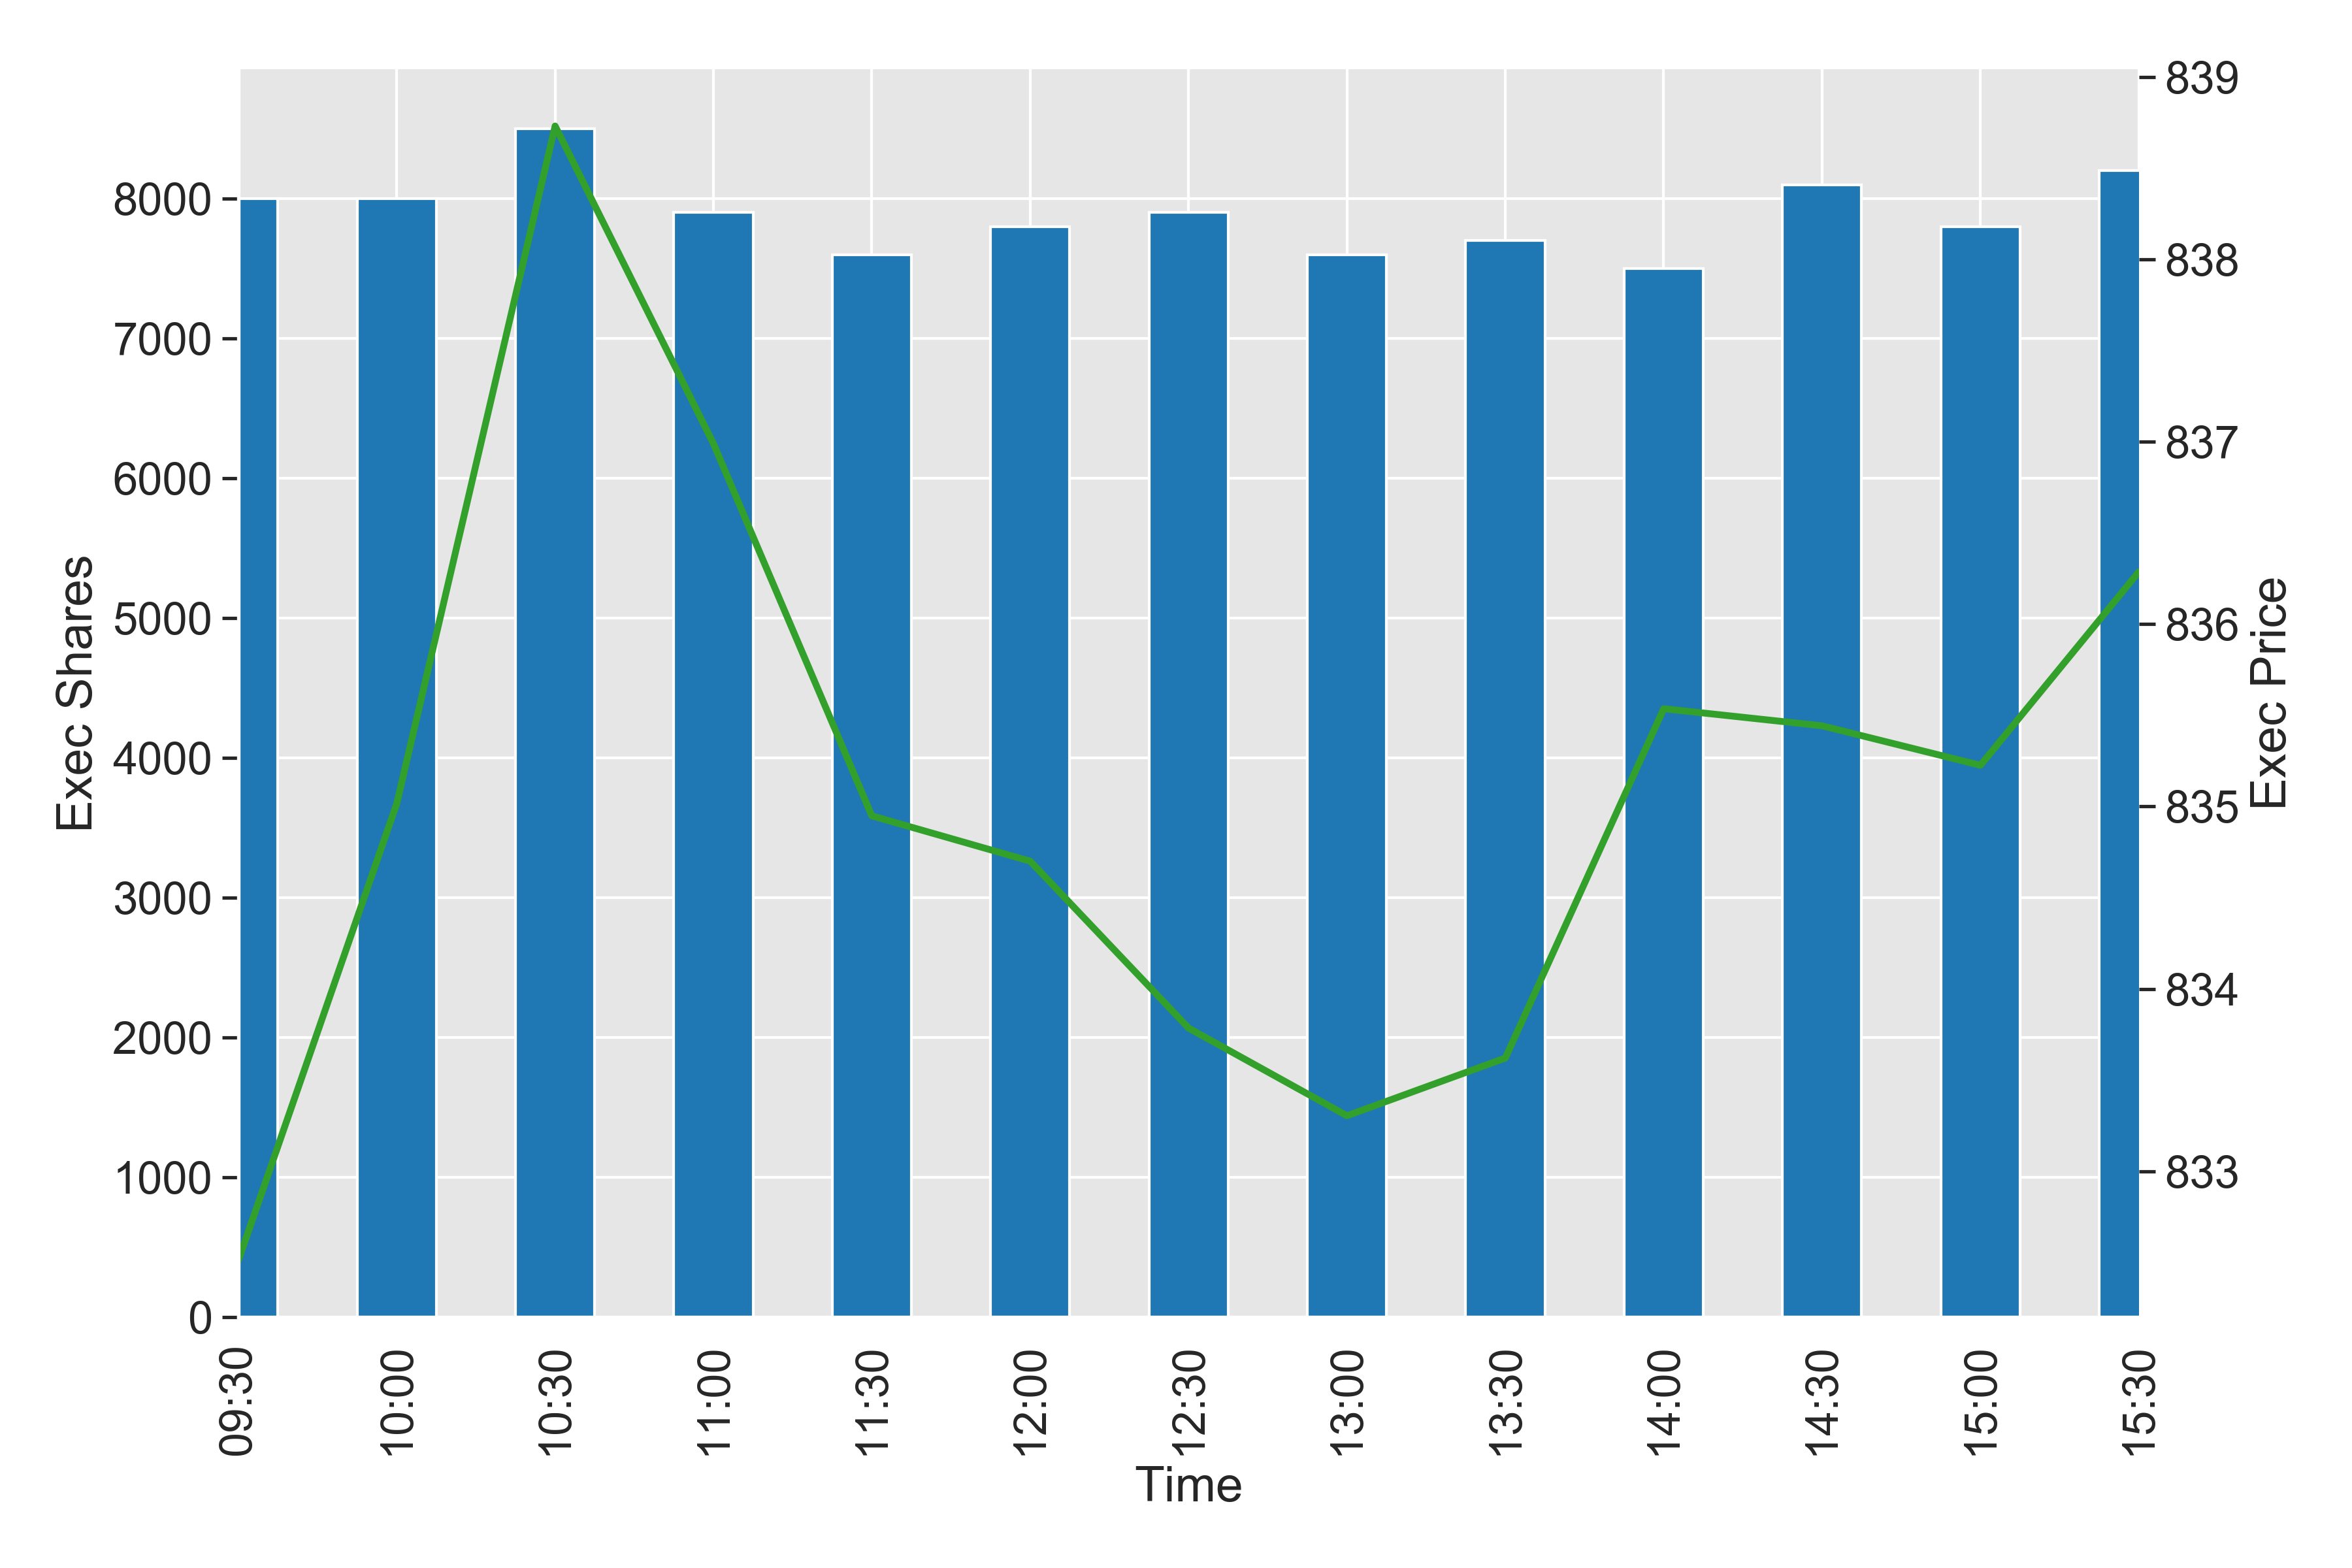
\includegraphics[width=\textwidth]{chapters/chapter_exec_models/figures/twap.png} 
        \caption{Example of TWAP Trade for AMZN. \label{fig:vwap}}
        \end{figure}


\noindent\textbf{VWAP} \twomedskip


The Volume Weighted Average Price (VWAP) is the next simplest benchmark that is commonly used. Simply weigh every trade by the normalized trade size.
        \begin{equation} \label{eq:vwapstet}
        \text{VWAP}_{\text{st}} ^{\text{et}}= \dfrac{ \sum_{i=1}^N p_i^* s_i }{ \sum_{i=1}^N s_i }.
        \end{equation}
This benchmark  is arguably a better measure of the fair market price over the trading period (trading times and prices that are closer to the times and prices other market participants---who might have a better assessment of the short term price - trade). All the arguments for and against the VWAP benchmark are the same as the ones discussed for TWAP. 


The VWAP strategy, in order to achieve its goal, takes advantage of the relative stability of the volume distribution over the day we discussed in Section~\ref{s:profiles}. Instead of trading equally throughout, the time period the strategy splits the parent order proportionally to the volume profile re-normalized over the time horizon.


The VWAP strategy is conceptually superior to TWAP as a market impact reduction approach since by trading more (less) when more  (less) volume is expected to trade it does a better job at minimizing the realized trading rate. That being said if the volume profile is, for some special circumstances, extremely noisy or unpredictable, trading VWAP might actually be inferior to TWAP since the error in our volume profile prediction might cause the strategy to achieve a higher trading rate than the simpler strategy. This will emphasize the need for good volume forecasts for various discrete time intervals.


There is an argument to be made that, reiterating the lack of any price dynamic/prediction information, VWAP is the best approach to trade an order when the order needs to complete. For this reason the strategy is still one of the most used strategy by quantitatively driven funds in which the investment strategy correctly sizes the order to minimize overall impact. Generally, while in recent years the popularity of VWAP has decreased in favor of the more flashy ``Liquidity Seeking'' strategies, it is still one of the most used strategy in the market. We will discuss Liquidity Seeking strategies in a later section. \twomedskip


        \begin{figure}[!ht]
        \centering
        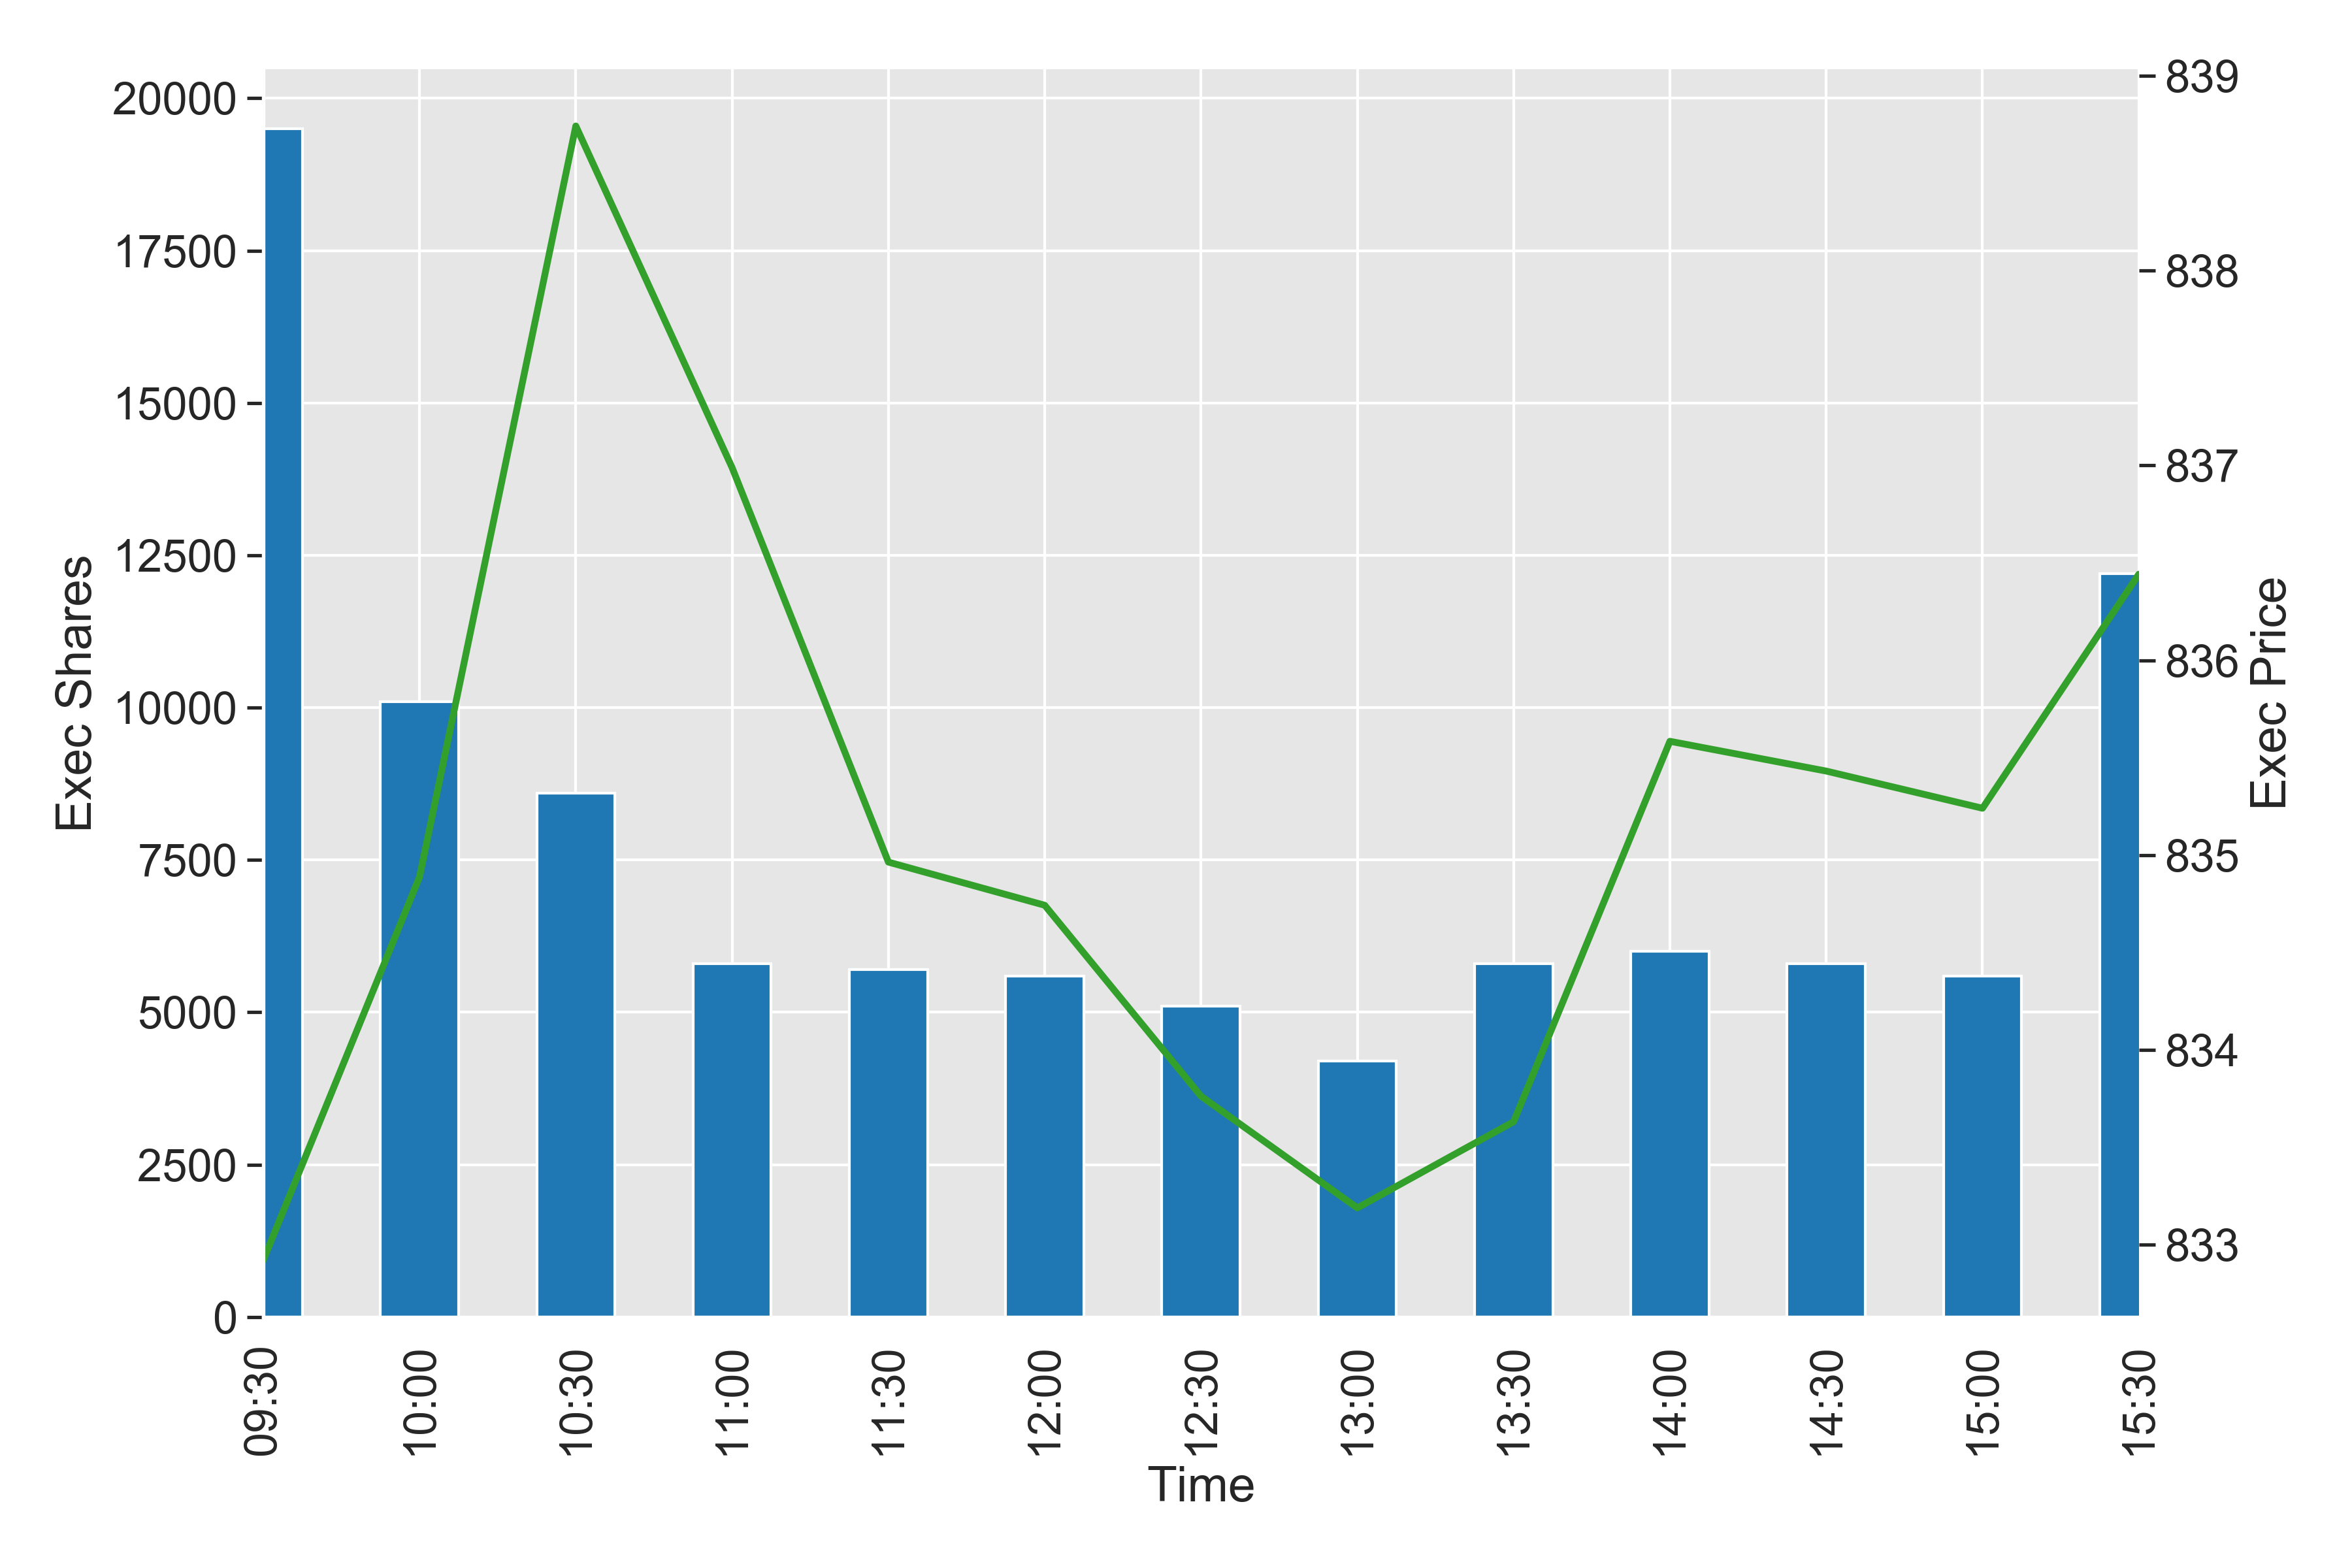
\includegraphics[width=\textwidth]{chapters/chapter_exec_models/figures/vwap.png} 
        \caption{Example of VWAP Trade for AMZN. \label{fig:vwap}}
        \end{figure}


\noindent\textbf{Inline with Volume, a.k.a. POV} \twomedskip


The previous paragraph hinted that one of the limitation of VWAP (and TWAP) as a market impact controlling tool in that they do not take into consideration the high degree of variability in the daily volume. If, in a particular day, the actual volume is significantly less than expected (due to lack of activity or large distortion in the volume profile) the VWAP strategy will just trade at a higher rate than originally envisioned by the trader leading to a higher total cost. Conversely, if trading a multiday order on a day where more volume is traded than expected, the trader would likely trade a smaller portion of the order than the market would have been able to absorb for the same expected impact cost.


If completing the order is an absolute hard necessity, arguably, there is little that can be done. However if there is some flexibility around completing the order then another approach can be taken. This is where Inline strategies come into play. Inline or alternatively called POV (Percentage of Volume) strategies have target trading rate as a benchmark and not a price. They aim at trading at a fixed rate as a way to directly control market impact. While seemingly straightforward, following a certain participation rate in real time is not at all an easy task and these strategies can have some severe drawbacks unless carefully implemented.


\begin{itemize}
\item Early implementation where purely reactive meaning they would observe volume for a certain period and then trade the prescribed portion of that volume in the next iteration. Due to the noise in the volume dynamics this could lead the strategy to oversize the market after a large volume spike. In particular, large block prints, if not correctly managed, can cause the strategy to severely over-trade

\item Even when a volume forecast is used there is still a lot of error in the estimates and any shortfall needs to be correctly managed and possibly smoothed over multiple periods to avoid excessive impact.

\item The POV benchmark is extremely noisy in particular at the beginning of the order due to the granularity of trading. This can lead to no trading at the beginning until enough volume is traded and then immediately chasing that volume aggressively because the strategy immediately we are likely to fall behind the target volume.
\end{itemize}


Because of these drawbacks and complexities Inline strategies have somewhat lost their popularity and the more flexible Liquidity Seeking approaches  have more or less taken their place.


The POV benchmark does not provide a way to measure effectiveness of the strategy as an impact prevention approach in particular because of the issues discussed above. The PWP $X$ (Participation Weighted Price at $X$\% of the market) price is used as a measure of execution quality for the inline benchmark. It represents the price one would have obtained had they traded $X$\% of the market volume until completion of the order (in practice, the VWAP of the period from order start until ($1/X \times$ Order Size) has traded in the market). \twomedskip

	\begin{figure}[!ht]
	\centering
	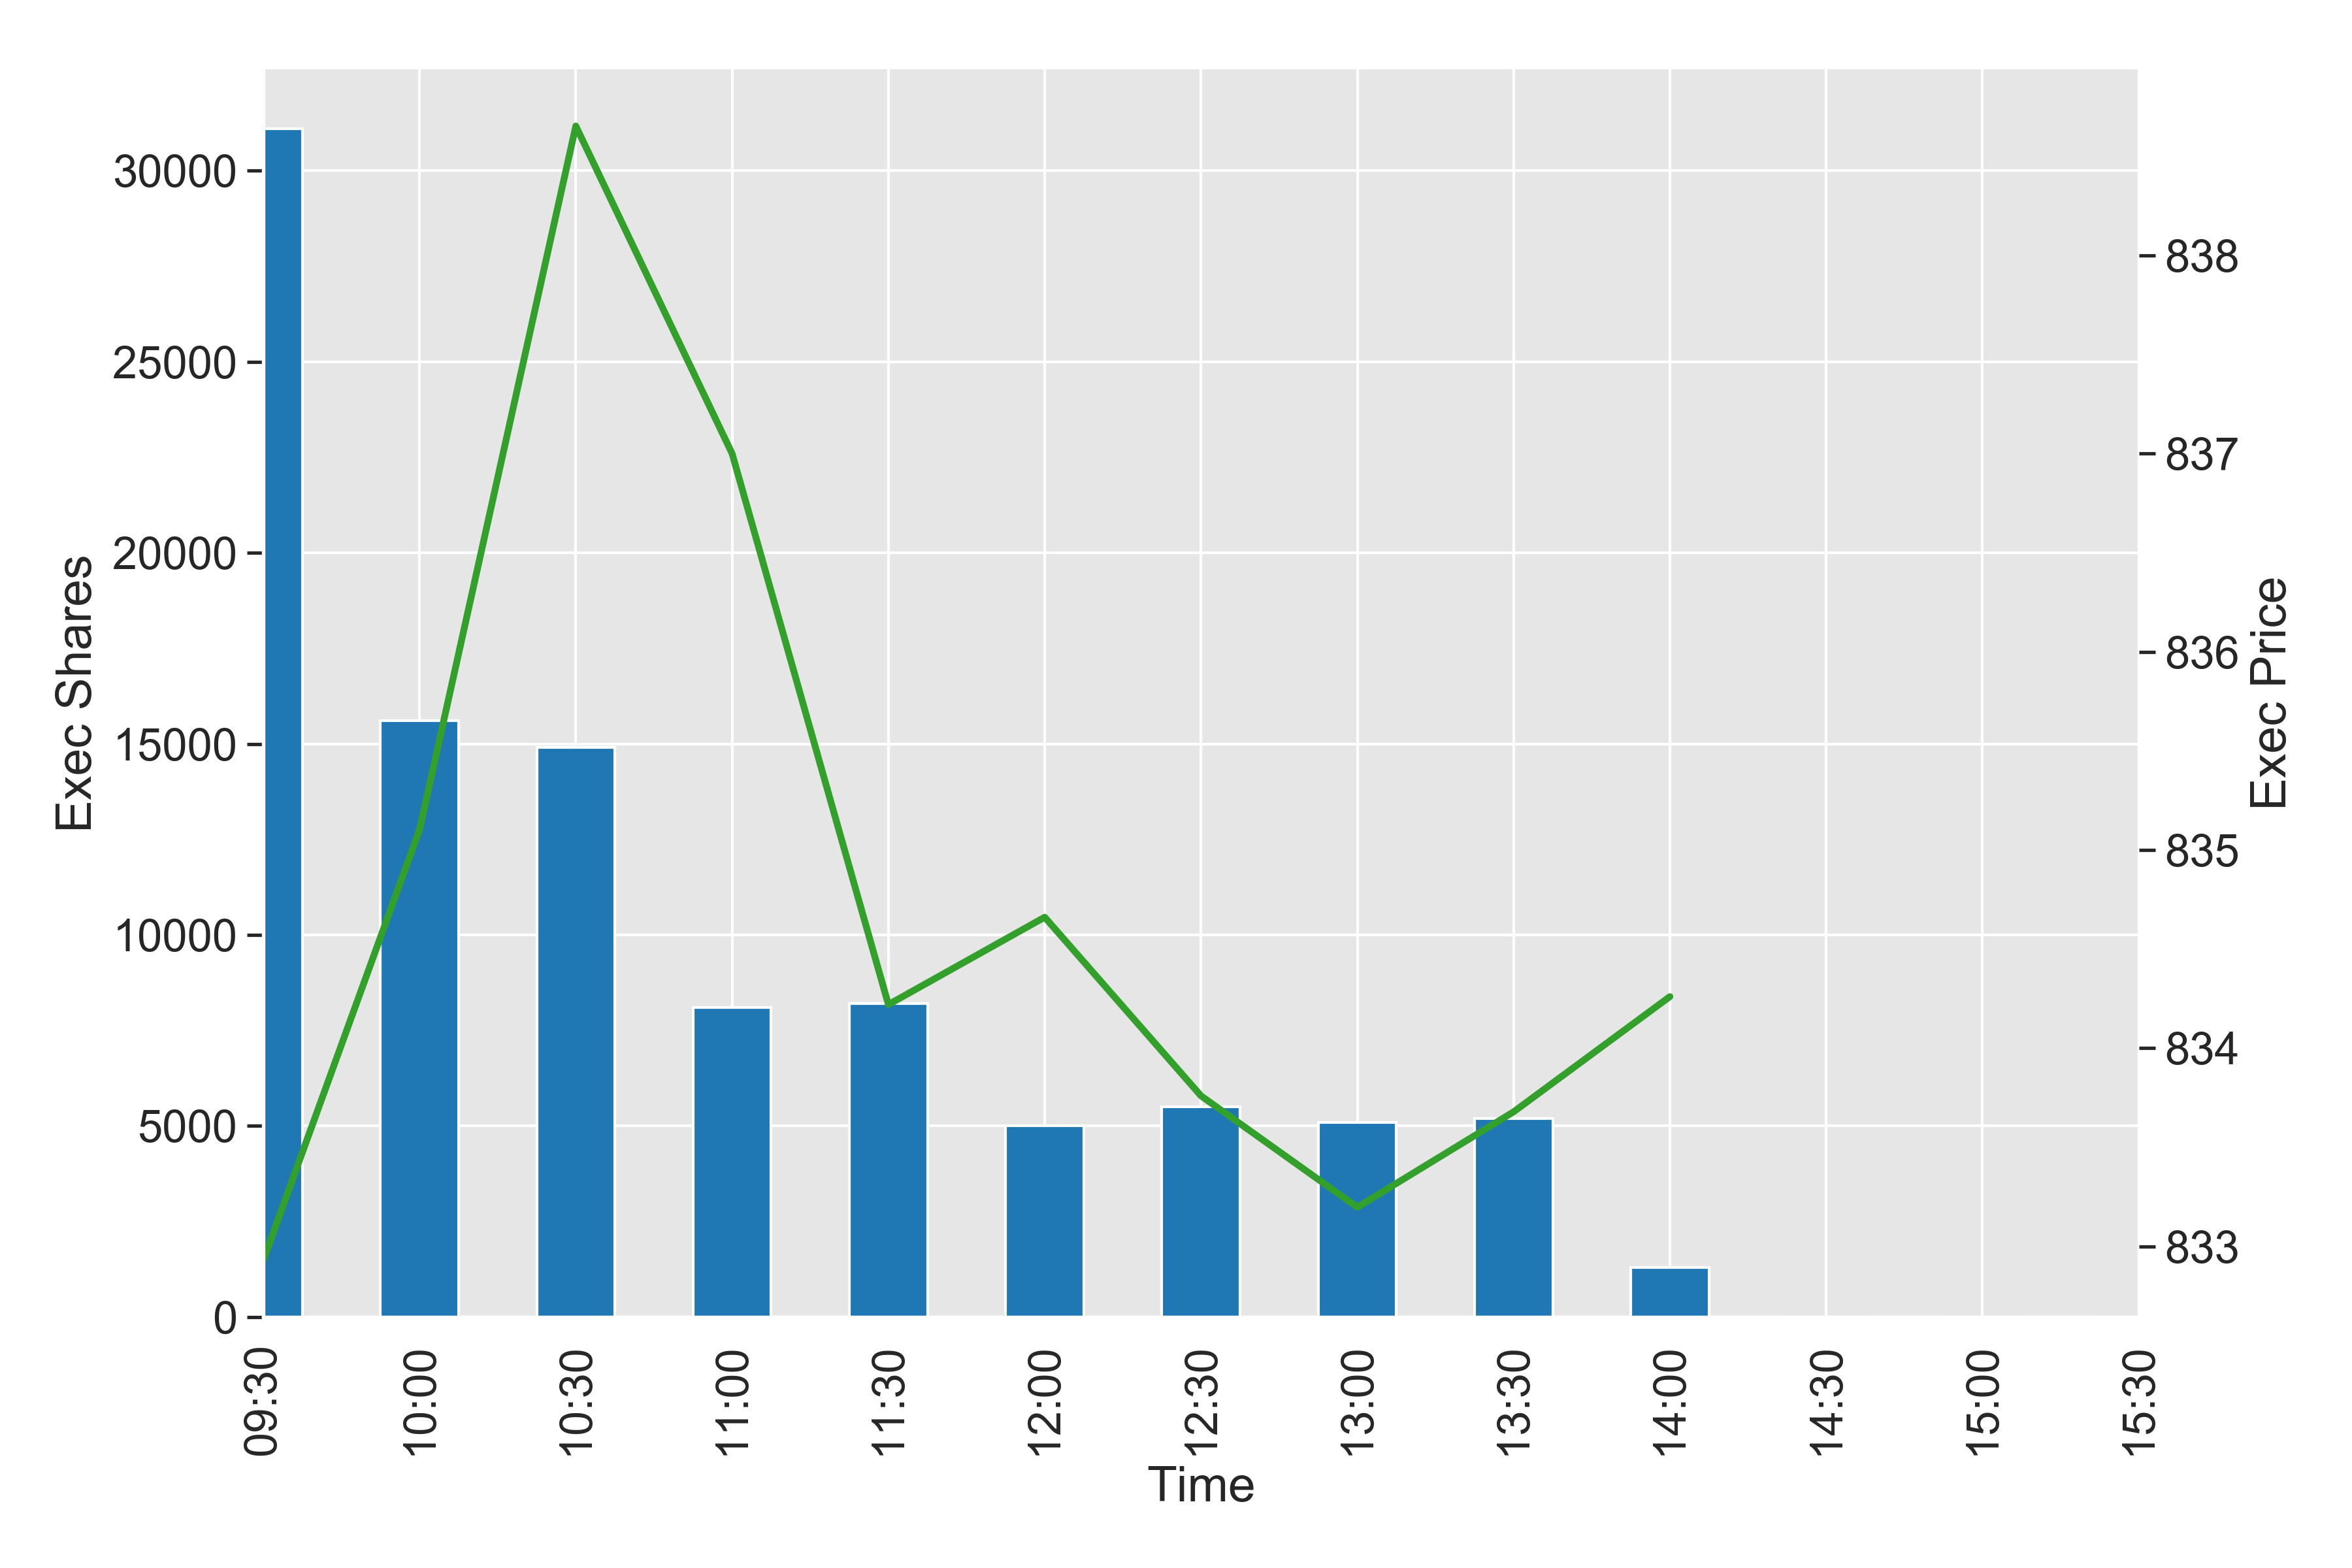
\includegraphics[width=\textwidth]{chapters/chapter_exec_models/figures/pov.png} 
	\caption{Example of 5\% POV Trade for AMZN. \label{fig:pov}}
	\end{figure}


\noindent\textbf{Target Close} \twomedskip


As previously discussed may quantitative strategies leverage time series data based on closing prices. As a result, some PM/traders favor this price point as a benchmark for the execution strategies. This is also the case for passive indexers whose fund tracking error is computed based on closing prices. This clearly places a particular importance to the closing price and thus the desire to minimizing the risk from large negative deviation from that price.


The Target Close strategy was devised to handle this use case. It is important to understand that in general even Target Close is an IS strategy in the sense that it still trying to achieve the elusive best price possible. If the ultimate price was unimportant the strategy would be trivial: place the whole quantity as a Market-on-Close (MOC) order into the closing auction no matter how big. The closing price could be negatively affected by the excess imbalance but the order WILL achieve the closing price benchmark. Instead the objective is to limit market impact while but trading at times closer to the end of the day limiting the risk of large deviations from the close price. Most strategies attempt to forecast the amount of closing volume and size the MOC slice accordingly thus limiting the chance of negatively affect the close price and then trade the rest in the latter part of the continuous phase accelerating the trading rate toward the close. \twomedskip

	\begin{figure}[!ht]
	\centering
	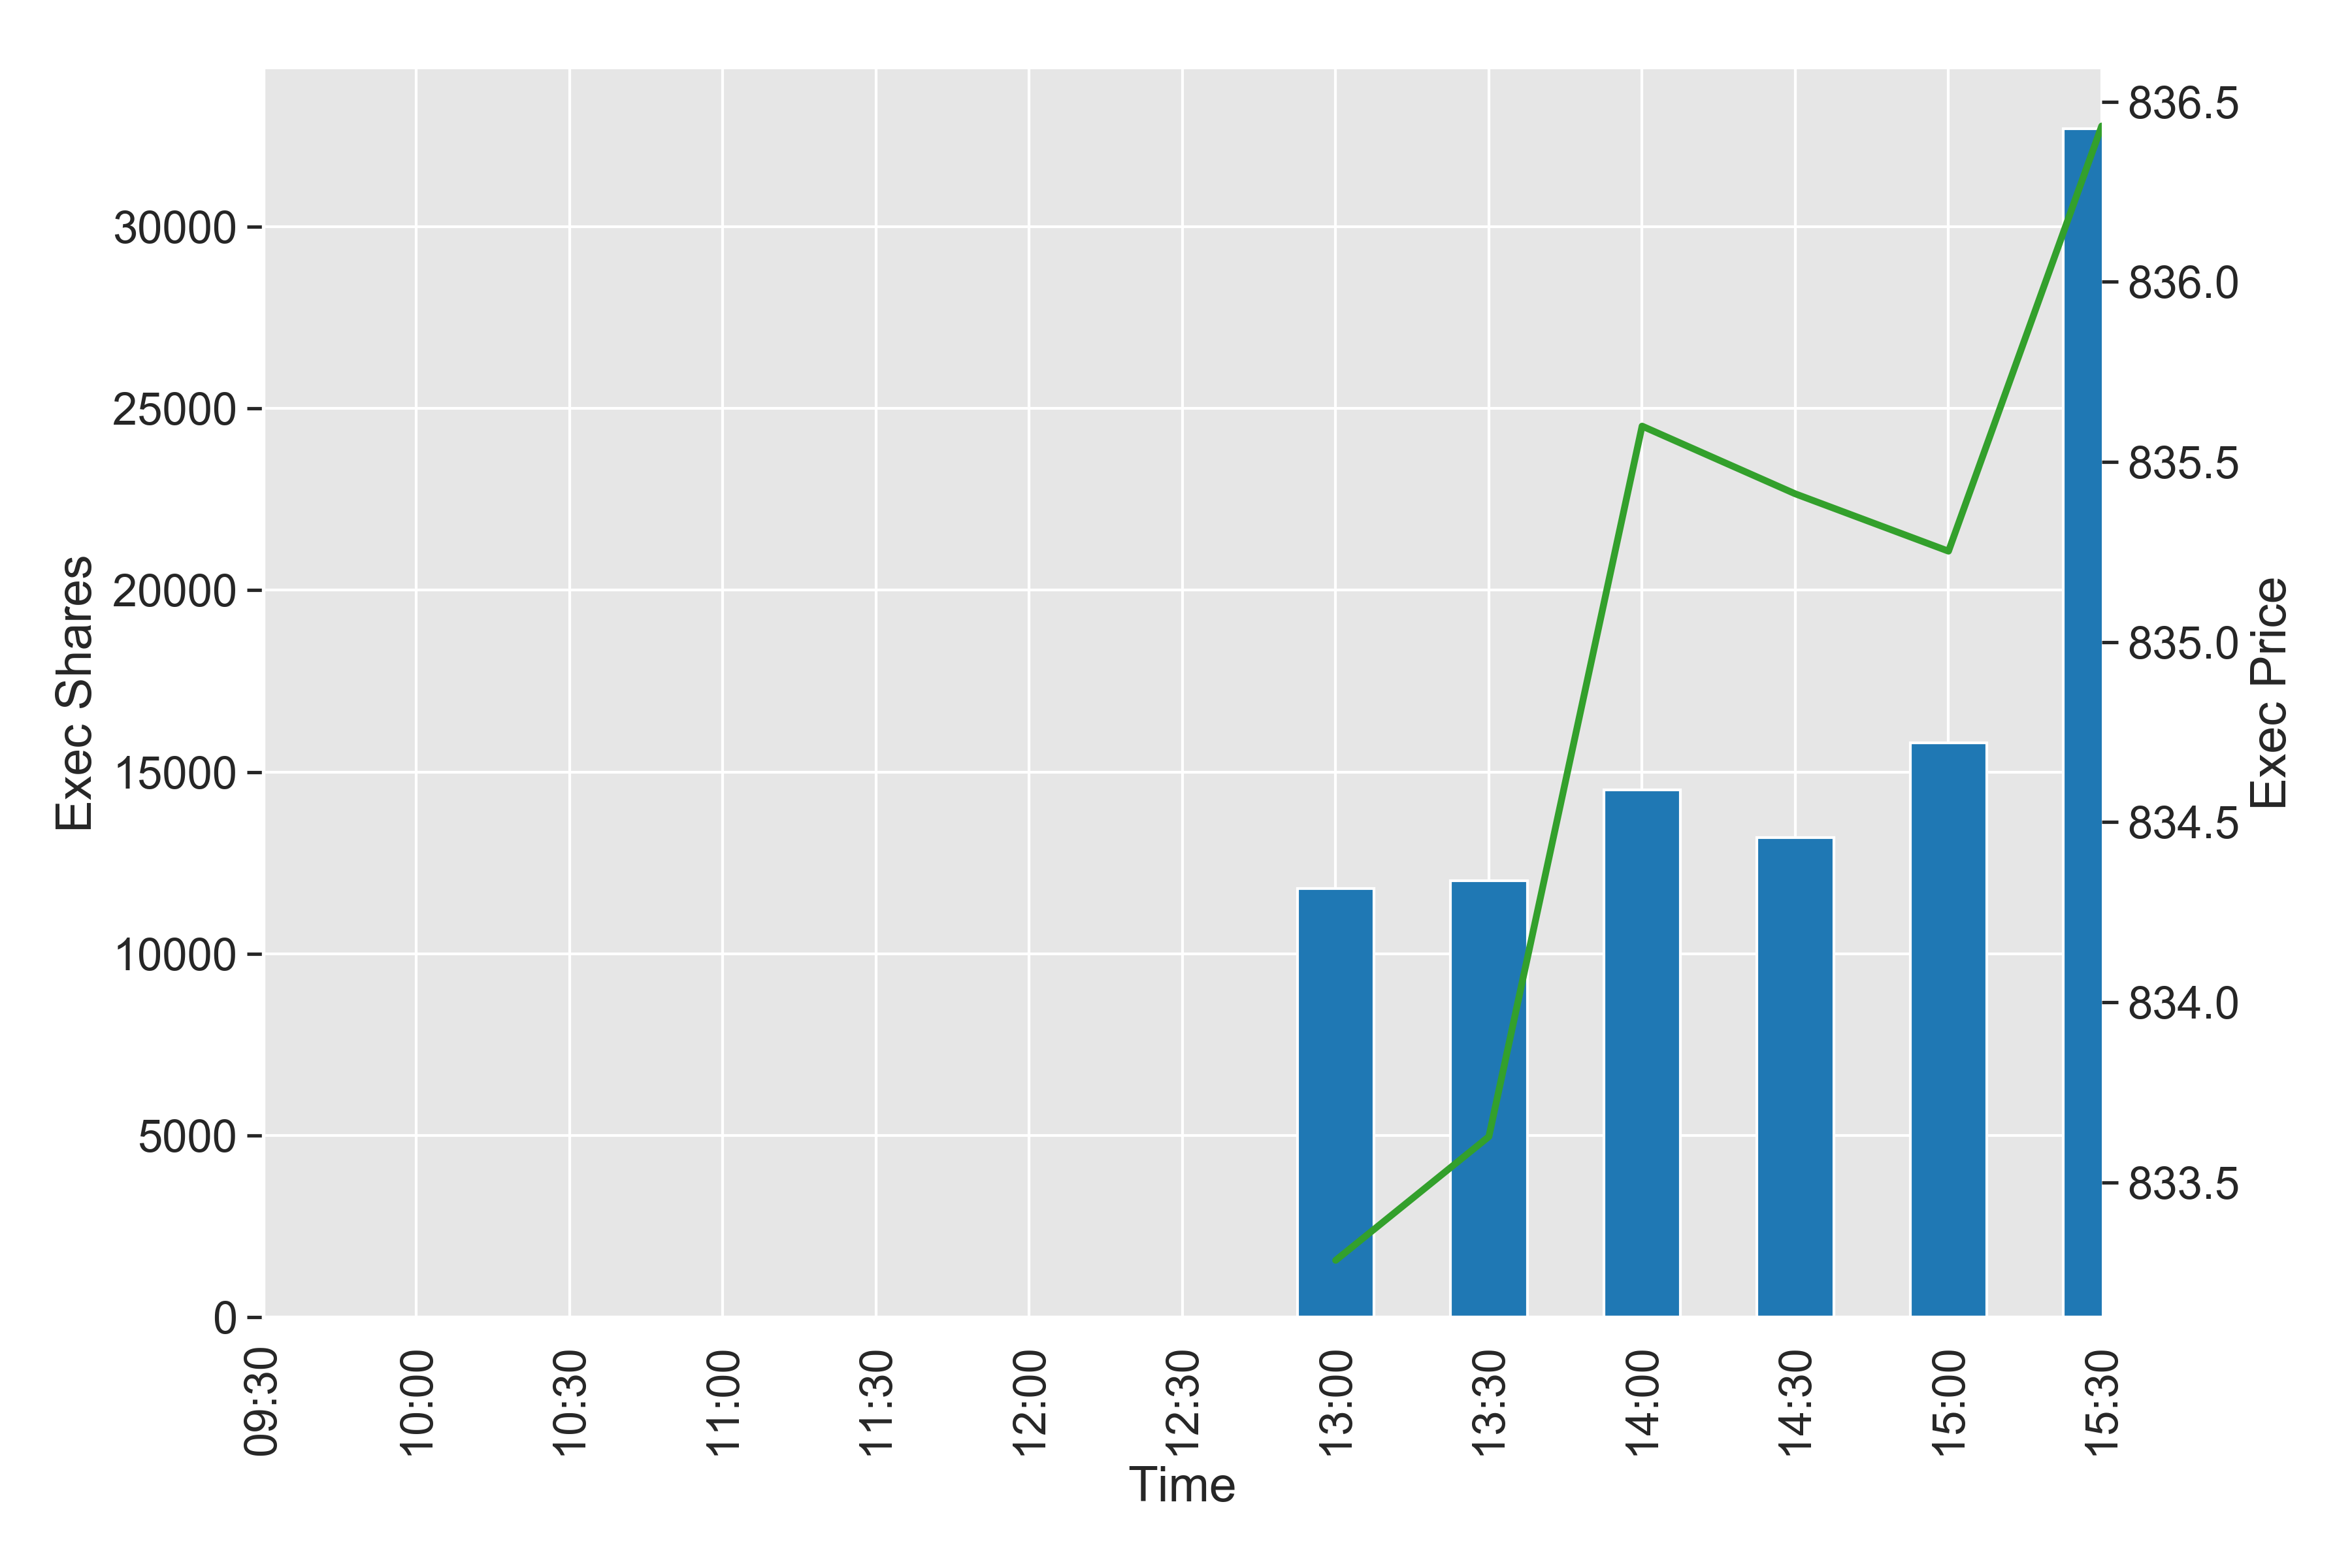
\includegraphics[width=\textwidth]{chapters/chapter_exec_models/figures/close.png} 
	\caption{Example of a Target Close Trade for AMZN. \label{fig:close}}
	\end{figure}


\noindent\textbf{Auxiliary Benchmarks} \twomedskip


In addition to these standard primary benchmarks, several additional metrics are often used to shed more light on execution performance. Here is a non-exhaustive review:


\begin{itemize}
\item \emph{Spread Normalization:} As a way to make performance more  comparable across the stock universe the various benchmarks are often normalized by the prevailing spread. Intuitively the expected slippage of the same VWAP strategy trading two orders: one very liquid and with for 4bps spread and the other illiquid with a 20bps spread is likely to be very different. But as a \% of the period spread they will achieve more comparable results. 

\item \emph{Completion rate:} While achieving low slippage versus arrival price might be considered as a desirable outcome, if only a fraction of the parent order got executed, the user of the execution strategy is left facing a potentially significant opportunity cost as the expected alpha was not fully captured. In order to avoid rewarding strategies that achieve low implementation shortfall, just by being extremely passive and stopping trading when prices become unfavorable, most practitioners add a penalty term for the unexecuted portion of the order. There are several approaches to do so, one of the simplest being to apply a slippage to the unexecuted quantity equal to the difference between the arrival price and the closing price of the day. 

\item \emph{Close:} Even if not the central benchmark discussed above the closing price being the last accessible price of the day, it is often used to compute the opportunity cost for unexecuted quantity. 
There are different variations of this benchmark, most notably the previous day's close (for strategies that select their target holdings through an overnight process using the latest available close price as an input in their model) or the open price to reflect the fact the previous close is a price point that was not accessible to the strategy.

\item \emph{Make/Take ratio:} This ratio provides some indication of the execution efficiency. How much of the liquidity was sourced on the passive side of the spread (at the bid or lower for a buy order), versus how much was required for the algorithm to pay the spread? This metric highlights the quality of the order placement of the execution strategy through its ability to source liquidity while achieving its desired trading rate. It is worth noting, however, that more passive fills do not guarantee overall better performance with regard to the primary benchmark. For instance, if a security exhibits strong intraday adverse momentum, a very passive strategy favoring passive fills would likely result in lower participation rates, hence delaying the total execution and exposing the traders to unfavorable prices later in the day. Additionally as well performing strategy that leverages short term signals to trade more aggressively when prices move away and canceling passive orders to avoid adverse selection would score unfavorably on this benchmark. In general the reader is encouraged to remain critical when analyzing performance benchmarks and metrics, and strive to create more sophisticated versions that more accurately capture existing trade offs.

\item \emph{Mean vs. Variance of performance:} While absolute performance tends to be the main focus of execution benchmarking, a trader might also want to control its variability. In practice, traders with large amounts of flow on a daily basis often focus more on the attained mean as their risk of being adversely affected by outliers is somewhat mitigated by the number of orders. Conversely, occasional traders are often willing to accept a slightly less optimal average performance if it is accompanied by less variance.

\item \emph{Reversion:} An additional way to analyze market impact or short term opportunity cost is to study the stock price trajectory after the execution is completed. A sustained high demand for liquidity results in a displacement of the Supply-Demand equilibrium, as liquidity providers need to manage their inventories, that may lead to an adverse price move (market impact). Empirical evidence (as mentioned in Gatheral (2010)~\cite{gatheral}) suggests that the temporary component of price impact reverts once the execution stops, and the impact function follows a power law decay function. Hence, studying reversion at a time window commensurate with the order duration informs the trader of the impact cost that may have been incurred due to a participation rate. This rate might not be adapted to the liquidity that the market was able to provide at the time of the transaction.


%%%%%%%%%%%%%%%%%%%%
%%%%%%%%%%%%%%%%%%%%
\begin{comment}
\item \emph{Order Routing Performance:} Fragmented markets, whether due to the existence of several lit venues or numerous dark pools, add an extra layer of complexity. In a fragmented market, the routing decisions become important to optimal liquidity sourcing. Sending a passive child order to a venue and resting it there for a period of time without getting any execution while transactions happen elsewhere in different venues might incur opportunity cost if the market moves away and the child order ends up being traded at a less favorable price later on. Similarly, if the algorithm sends an aggressive child order to capture liquidity on the far touch, routing decisions as well as the speed of the router will affect how much of the displayed liquidity at the time of decision can be captured (fill rate). Other market participants, particularly high frequency market makers, tend to display liquidity on multiple venues simultaneously and are likely to attempt to cancel all other outstanding child orders once they receive the execution confirmation from the first hit venue to avoid adverse selection, and may replace their quotes deeper in the book. Hence, the trading algorithm attempting to capture all visible liquidity on the far touch at a point in time might end up only in a partial execution and may have to trade the remainder at a less favorable price. Given the volume and complexity of events to process in a fragmented market environment and the sensitivity to latency, the routing decisions are often delegated to the Smart Order Router (SOR) rather than handled by the algorithmic strategy itself. Most advanced SORs handle real-time market data feeds from various venues and incorporate estimations of the distance separating them from the matching engines of these venues in order to optimize child order routing sequence. Some of the common metrics used to measure performance of liquidity sourcing include analyzing fill rate on aggressive limit orders (higher fill rate meaning a more efficient routing), the ratio of routed versus executed quantity, and average time to fill in passive orders (less unsuccessful routing and shorter time to fill meaning less potential opportunity cost incurred by child orders).
\end{comment}
%%%%%%%%%%%%%%%%%%%%
%%%%%%%%%%%%%%%%%%%%
\end{itemize}



% Evolution of Execution Strategies
\subsection{Evolution of Execution Strategies}

The previous section described the main approaches used by the original algorithms that still account for the majority of the trading flow going through execution products around the globe.These strategies are conceptually simple but overall quite effective. While over time they evolved in sophistication with better analytics, order placement, and more nuanced handling of the schedule, the approach to the strategies has largely remained the same. As the business evolved, practitioners started looking for better approaches, something that would have some quantitative underpinning that would move beyond the na\"ive methods of these historical algorithms. We briefly look at how these efforts have evolved and the drivers behind this evolution. \twomedskip


\noindent\textbf{Implementations Shortfall} \twomedskip


At the turn of the century things changed with the seminal paper from Almgren and Chriss (2000)~\cite{alm2000} that proposed an approach to ``optimal execution.'' Finally, a more formal quantitative treatment of the subject. The approach was based on a  mean-variance optimization framework similar in spirit with the Markowitz optimal portfolio allocation setup.


We will discuss the  mathematical setup and results in the review of  academic literature on optimal execution. Here we limit ourselves to the high level discussion. The optimal schedule, claim Almgren and Chriss, is one that trades-off minimizing impact with the volatility of the overall cost. Like in Markowitz, the trade-off between mean and variance is governed by a hyper-parameter, `$\lambda$', which was meant to incorporate the ``risk aversion'' specific to a particular trader. Since the overall volatility cost depends on the remaining quantity, the variance is highest at the beginning of the order and thus the optimal schedule will trade-off more impact cost and thus a higher trading rate to reduce that variance. As the position decreases the risk decreases and thus the optimal schedule reduces its trading rate. The optimal schedule displays a very typical front loaded shaped trajectory that vanishes to zero at the trading end time.


The approach generated a vast amount of interest in the industry and brokers increased their investment in quantitatively strong personnel who could understand and implement these strategies leading to the evolution of a new type of quant: the execution quant. Most algorithm providers implemented a version of this algorithm and hailed the arrival of the ultimate solution to the IS problem. The incredible popularity of the approach led to a dramatic increase in the interest of the academic community to find better approaches to the Optimal Execution problem. We will discuss the highlights of the evolution of the optimal execution field of study in the next section. It is important to note that, because the approach is fundamentally based on the dynamics of market impact, this renewed interest from academics had  a hugely important side benefit of a significant increase in the research around market impact models. 


The approach had its detractors. Many traders were highly skeptical of the approach because they did not believe that a completely static approach, could be the optimal way to trade without taking into account what is happening in the market. These traders would claim that a real IS strategy should be dynamic, ``picking spots'', backing off when prices are not favorable and take advantage of prices.  Additionally, the dramatic increase of dark liquidity that promised the ability to trade in large positions with zero (limited) impact, further challenged the idea of a static schedule to achieve the best price possible. Finally, the actual implementation was often problematic because it did not account for the possibility of the order being amended. Because most algorithms' infrastructures, when a parameter is changed, do not maintain any state and they react by creating a brand new parent order. The IS optimization will then re-evaluate the strategy and front-load again the schedule creating further impact on the stock. For traders that use tight limits, this created real havoc.


Some buy-side quants were also skeptical. They correctly argued that the IS schedule, by being a mean variance trade-off, is actually not providing the best price. The optimization trades off some expected cost for a reduction in the uncertainty of the outcome (i.e., standard deviation). But to large trading operations, the average shortfall is really the only thing that matters. They would gladly take additional volatility if they could achieve a better price. In this setting their risk aversion is zero. What happens when, in this elegant quantitative model, one sets a zero risk aversion? In this case the reduction in market impact is the only component in the optimization and the Almgren-Chriss' model reduces to\dots  wait for it\dots VWAP! So a large subset of users shrugged off the revolution and continued to use VWAP as their main approach.


Execution quants struggled to adapt the IS framework to incorporate the feedback. The restrictive mathematical framework made it complex and awkward to evolve. Several providers kept the ideas but abandoned the original formulation, others tried to incorporate more dynamic approaches by moving to a stochastic control framework. Some still kept the original formulation fixed and bolted on a set of heuristics.


New academic work expanding on the framework is now available; however, the solutions often appear non-intuitive such as: ``The optimal trading approach is to trade a large portion of the order at the beginning and the end of the time horizon with only moderate trading in the middle''. These new results have generally not been adopted by practitioners yet as they considered them to be somewhat unrealistic. While the debate is still ongoing and there are a few IS implementations that follow the original framework. The approach is slowly falling out of favor in favor of a more dynamic set of algorithms. \twomedskip

	\begin{figure}[!ht]
	\centering
	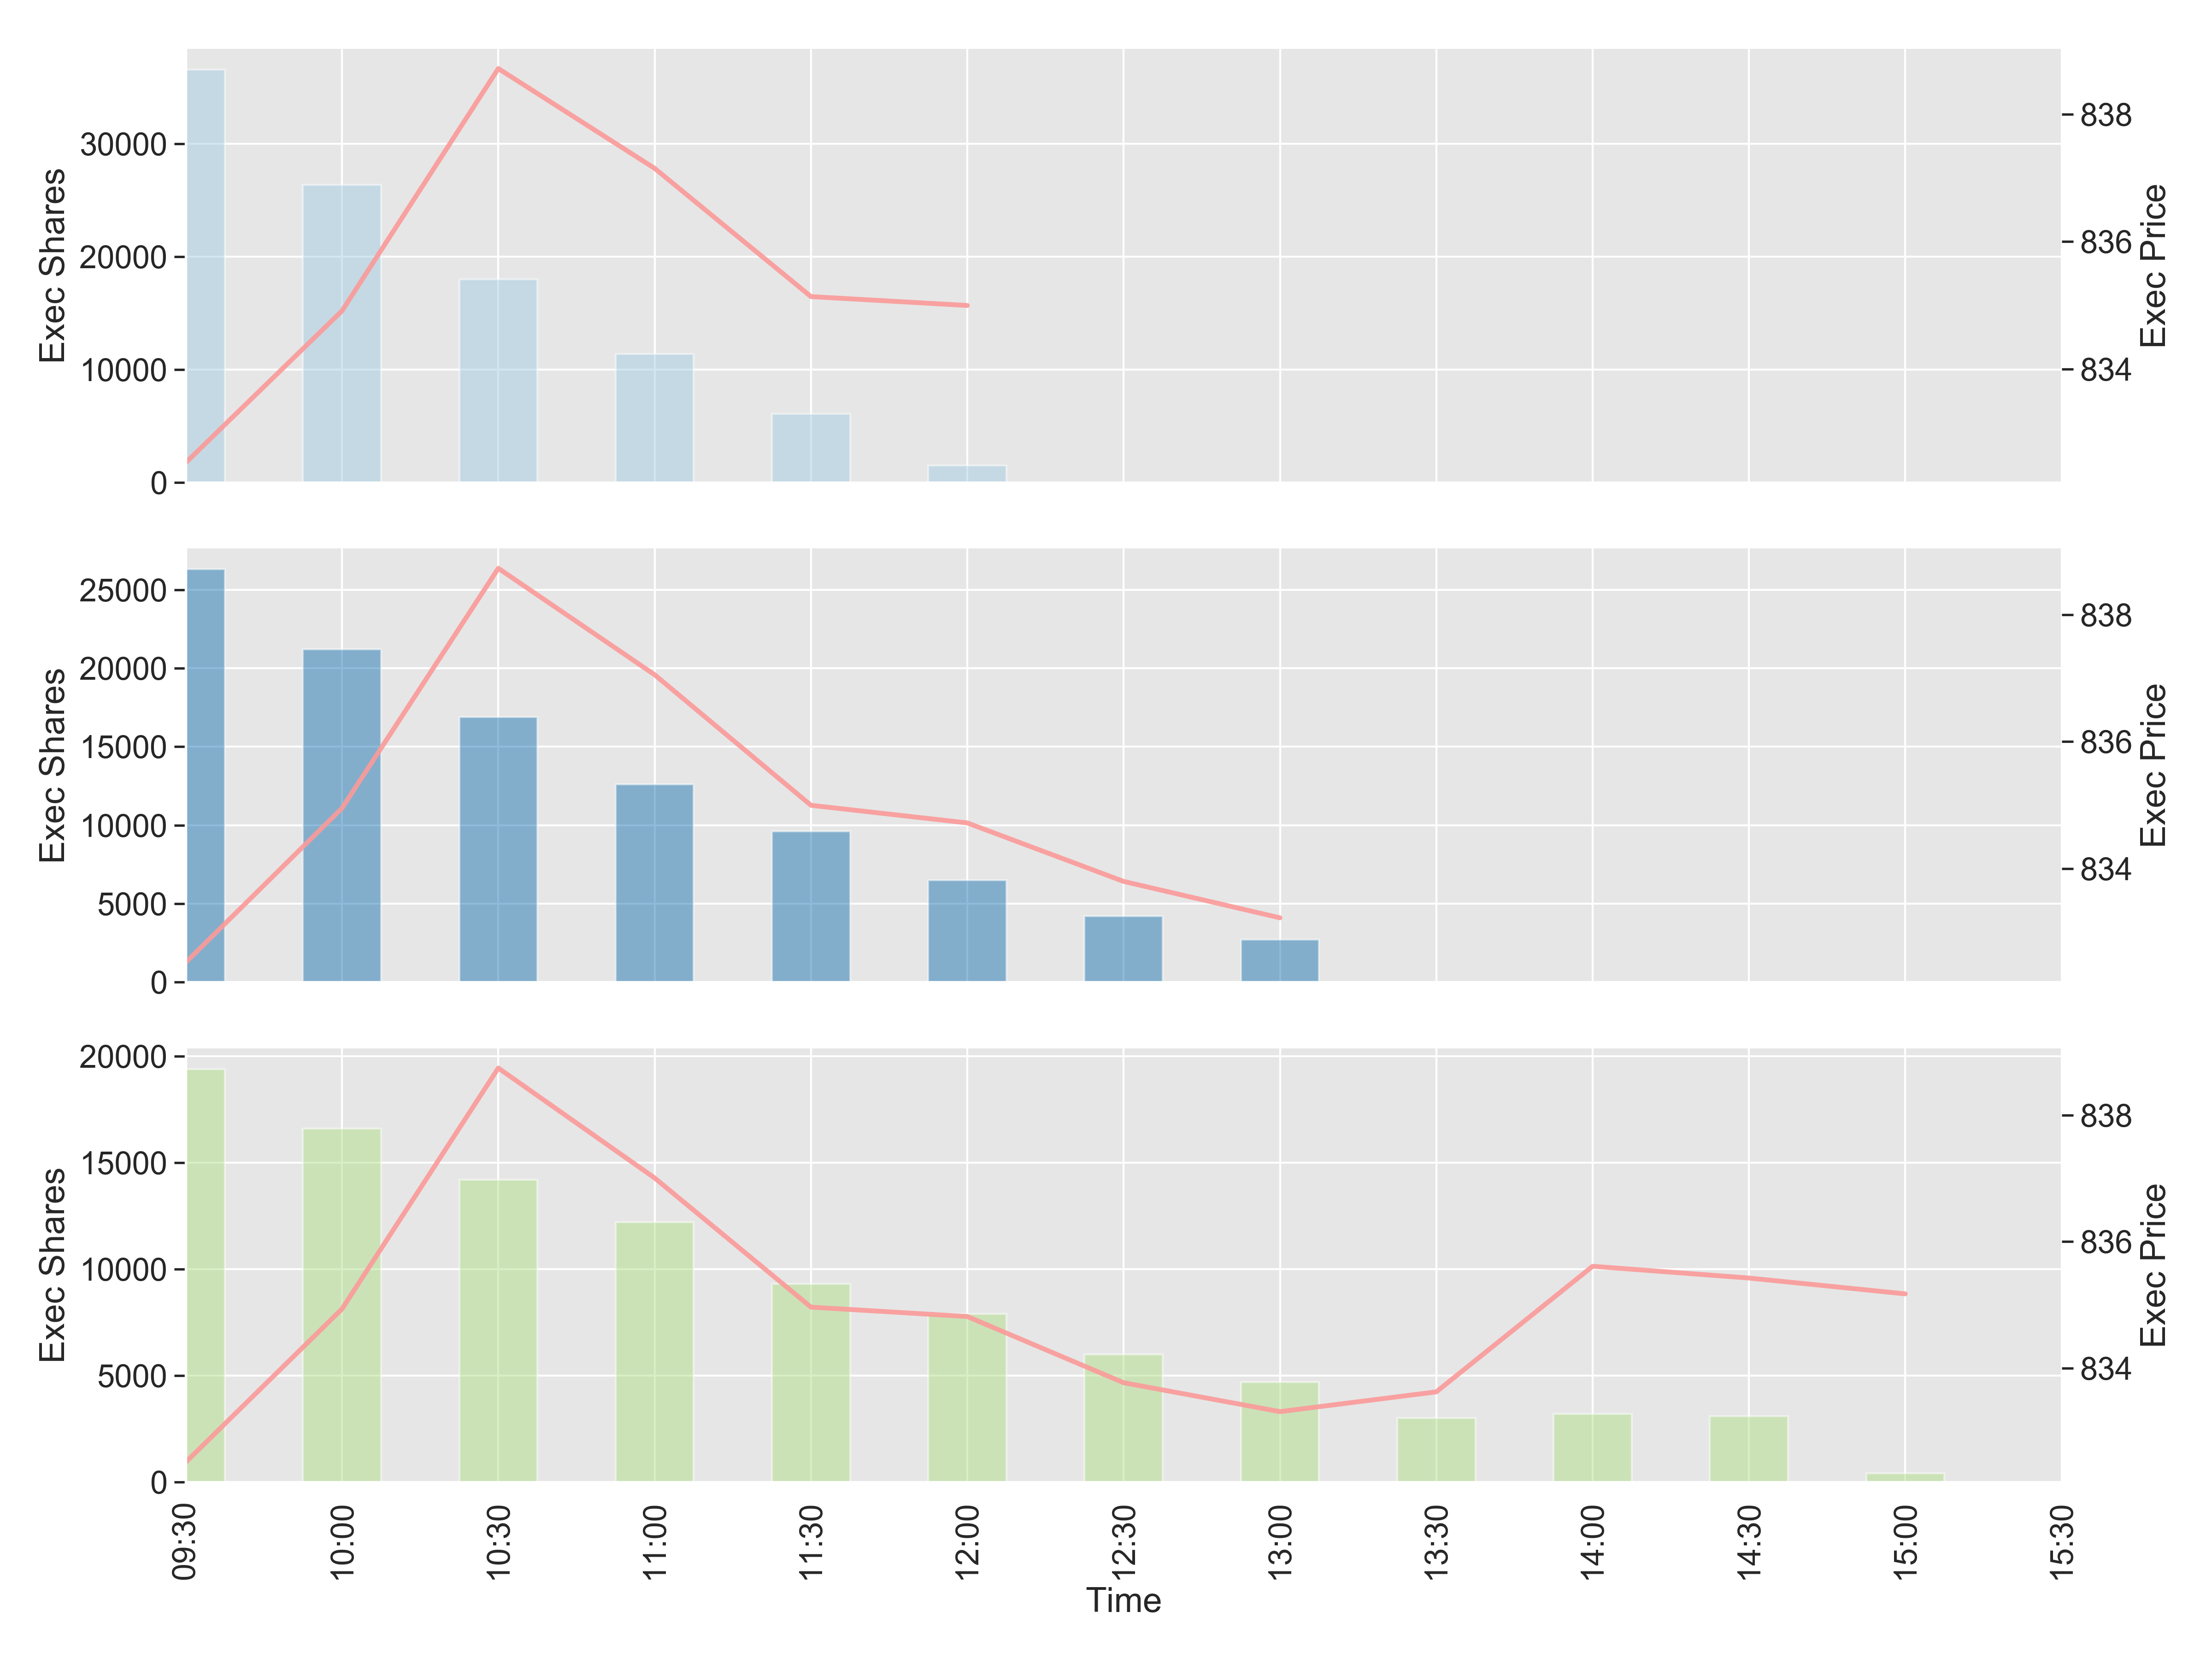
\includegraphics[width=\textwidth]{chapters/chapter_exec_models/figures/is.png} 
	\caption{Almgren \& Chriss' solution for different risk aversions. \label{fig:is}}
	\end{figure}



\noindent\textbf{Liquidity Seeking Algorithms} \twomedskip


The next generation of algorithms, broadly named Liquidity Seeking, are to some extent a rejection to schedule-based approaches that had dominated up until then. This came as a recognition that often these approaches have to make sub-optimal decisions in order to purely maintain a schedule and these decisions have significant impact on the performance of a strategy. By abandoning the schedule for a completely dynamic approach it is hoped that the excess impact due to ``schedule catch-up'' behavior would be reduced.


Liquidity Seeking algorithms encompass a range of approaches and urgencies from very aggressive, taking as much liquidity as possible up to a certain maximum limit price, to strategies that post all liquidity in dark pools, to highly opportunistic strategies that pounce at particular situations in the market such as far-side outsized liquidity (i.e. when the visible quantity at the far side is unusually large),\footnote{Far side outsized liquidity is essentially similar to quote imbalance which, we discussed, points to the price going in the favor of the order. For this reason taking that liquidity at that price would seem counter-intuitive and, while this is a common practice,  there is little to no evidence that the approach is highly beneficial.} to everything in between.


The downside of these approaches is that, since there is not a schedule to follow, the behavior can be highly non-deterministic and it implicitly excludes any timing risk component. The order that does not find enough liquidity would remain, possibly to a large extent, incomplete. That order would then have to be traded the next day. To address that traders started demanding that the algorithm maintains a minimum participation rate thus reintroducing an underlying scheduling component. Another common issue, in particular in the early days, is the tendency of maintaining a large portion of the order hidden at the midpoint which results in the tendency of severe  adverse selection. If the residual of a large order is fully executed at the midpoint, there is a high degree of probability that the price immediately after the trade would have been be more attractive, and thus creating a regret. This led some traders to demand that even in the dark pool the order should be ``paced'', again reintroducing the concept of a schedule.


In the last few years,  innovation on execution trading styles  has somewhat tapered off. This slowdown in new algorithmic approaches is partly due to the push of many buy side trading desks towards a more predictable and systematic attitude toward strategy and algorithm providers selection. The so-called ``Algorithm Wheels'' are becoming more and more popular in large buy side institutions as their requirements for demonstrating best-execution call for a simpler and homogenized trading approaches. They want to efficiently use as much of the sample set to make data driven decisions. 


Competition is as fierce as ever due to recent regulatory changes driven by Europe's MIFID~II regulation. However, the focus has mostly be on improving the various underlying components, looking for more sophisticated approaches that can further squeeze out performance from existing strategies. To some extent, sophisticated traders have started to move away from strategies and towards more abstract objectives and constraints allowing brokers to pick the best approach to achieve them. They engage with the algorithm providers with unprecedented openness in their effort to further minimize the overall trading costs. The benchmarks have not changed and can be still confusing and elusive; however, relative performance is easy to measure thus at least workable. This new freedom to experiment and single-minded focus on performance is leading to a renewed energy and innovations that could signal a new ``Golden Age'' of electronic trading.



% Layers of an Execution Strategy
\section{Layers of an Execution Strategy}

Having reviewed the basic approaches for execution strategies we turn our attention to how these strategies are actually implemented. To a very large extent the approach to all strategies is somewhat homogeneous and can be decomposed in a set of trading concerns that are well understood and to some extent can be looked at separately. In this section we review these layers one by one providing the high level concepts around standard and more modern approaches.


% Scheduling Layer
\subsection{Scheduling Layer}

This layer is responsible for actually implementing a particular strategy. Often described as the macro trader of the strategy, it is in charge of decisions spanning the whole order duration such as allocating the parent order quantity through the life of the order. It answers the question: ``how much should I trade in each period?''. The scheduler is aware of the overall trading intention, total quantity to transact, strategy parameters, constraints (maximum POV, limit price), and order duration. Taking the example of a VWAP algorithm, the scheduler is the component in charge of following the prescribed volume curve between the start and end times provided by the user. To derive the allocation, most schedulers discretize the trading horizon in more or less granular bins (generally one to five minutes), each considered a distinct trading interval to be handled by the child order placement module.


The scheduler will also need to decide which market phases should the algorithm interact with if not specified by the user. For instance, participating in auctions or not. For illiquid names, call auctions can be a significant source of liquidity so participating in them can limit the need for excessive trading in the continuous session. However, trading too much in the open auction---for example---can create an anchoring effect leading to a more permanent market impact, price displacement for the remainder of the continuous session, thereby negatively impacting follow-on executions. As often in electronic trading, there are not always absolute solutions, but only trade offs.


The scheduling layer plays an important role in  implementing liquidity sourcing preferences, such as how much to participate in volatile periods of price discovery when spreads are wide (e.g. in the first few minutes after the market open), or allocating volume between lit and dark venues (where one trades certainty of execution for lower price impact). As discussed in Chapter~\ref{chap:ch_trade_data_models}, algorithms are leveraging many normalizing  variables in order to handle the different characteristics of the stock universe both on regular days and special days.  Modern scheduling layers are also responding to realtime feedback loops from the market and adjust their execution as necessary such front loading the execution if the market is expected to move unfavorably, or back load it in case of expected favorable move or adjust the balance across liquidity sources (lit or dark markets). 


In summary the scheduler's role is to organize, implement and adjust the overall plan of action for the strategy and it is clearly the most important component of a trading strategy. \twomedskip


\noindent\textbf{Implementing a Scheduler:} \twomedskip


The above description is very high level and does not provide much in the way of approach on how to build a Scheduler in practice. Unfortunately, we cannot cover all the intricacies and details of a real world implementation but we will strive to provide some main ideas used in practice and some issues faced by practitioners. There is no standard approach to build a Scheduler and this treatment might prove quite simplistic and unsophisticated. But this is one approach the authors have used in practice. \twomedskip


\noindent\emph{Na\"ive Approach:} We start with the simplest implementation possible and evolve from there. This will also help the reader understand the limitations in the approaches and how one can deal with them. As discussed above a schedule is often represented by a vector of equally spaced discretized bins. We postulate that for each strategy we are able to determine the quantity required for the next bin which for schedule based strategies this is almost always true.\footnote{For POV strategy, this could be based on the previous bin volume or a forecast of next bin volume.} Each time period we submit to the order placement layer the exact quantity required for the particular bin. We assume that the order placement will ensure completion of the bin quantity by the end of the allotted time. If, for some reason, the order placement cannot fulfill the request dues to limit price or POV constraints, the scheduler simply ignores it and moves on to the next bin. 


Clearly, this is a quite crude implementation that could lead to severe under-trading and is very likely to result in excess impact due to the immediate ``catch up'' at the end of each bin. Less liquid stocks are not likely to be able to fulfill the required liquidity within each bin exacerbating the amount of required catch-up. One could normalize the time bin by some multiple of characteristic time which would somewhat harmonize the behavior across the stock universe but it may not address the other significant limitation of this approach.


A slightly more complicated approach would be to allow the order placement layer to engage in a best effort approach trying to fulfill the desired quantity without ``forcing'' a hard catch-up. Any unfilled quantity would simply be added to the next bin. This will limit the excess impact but exacerbate the tendency for the order to fall way behind the desired schedule. Clearly a tradeoff is needed. As an additional drawback to this approach is that in some cases the scheduler will have the undesirable tendency of being behind schedule most of the times.\footnote{For POV order, it is possible to be ahead of schedule when using volume forecasts which at time will overestimate the expected bin volume.} \twomedskip


\noindent\emph{Trading Bands:} A common approach used to address the above-mentioned drawbacks is via the introduction of trading bands. These are essentially auxiliary schedules above and below the desired schedule which represent how much behind and ahead the scheduler is allowed to deviate from the desired target. Figure~\ref{fig:schedule} shows a visual representation of a VWAP schedule with its trading bands. 

	\begin{figure}[!ht]
	\centering
	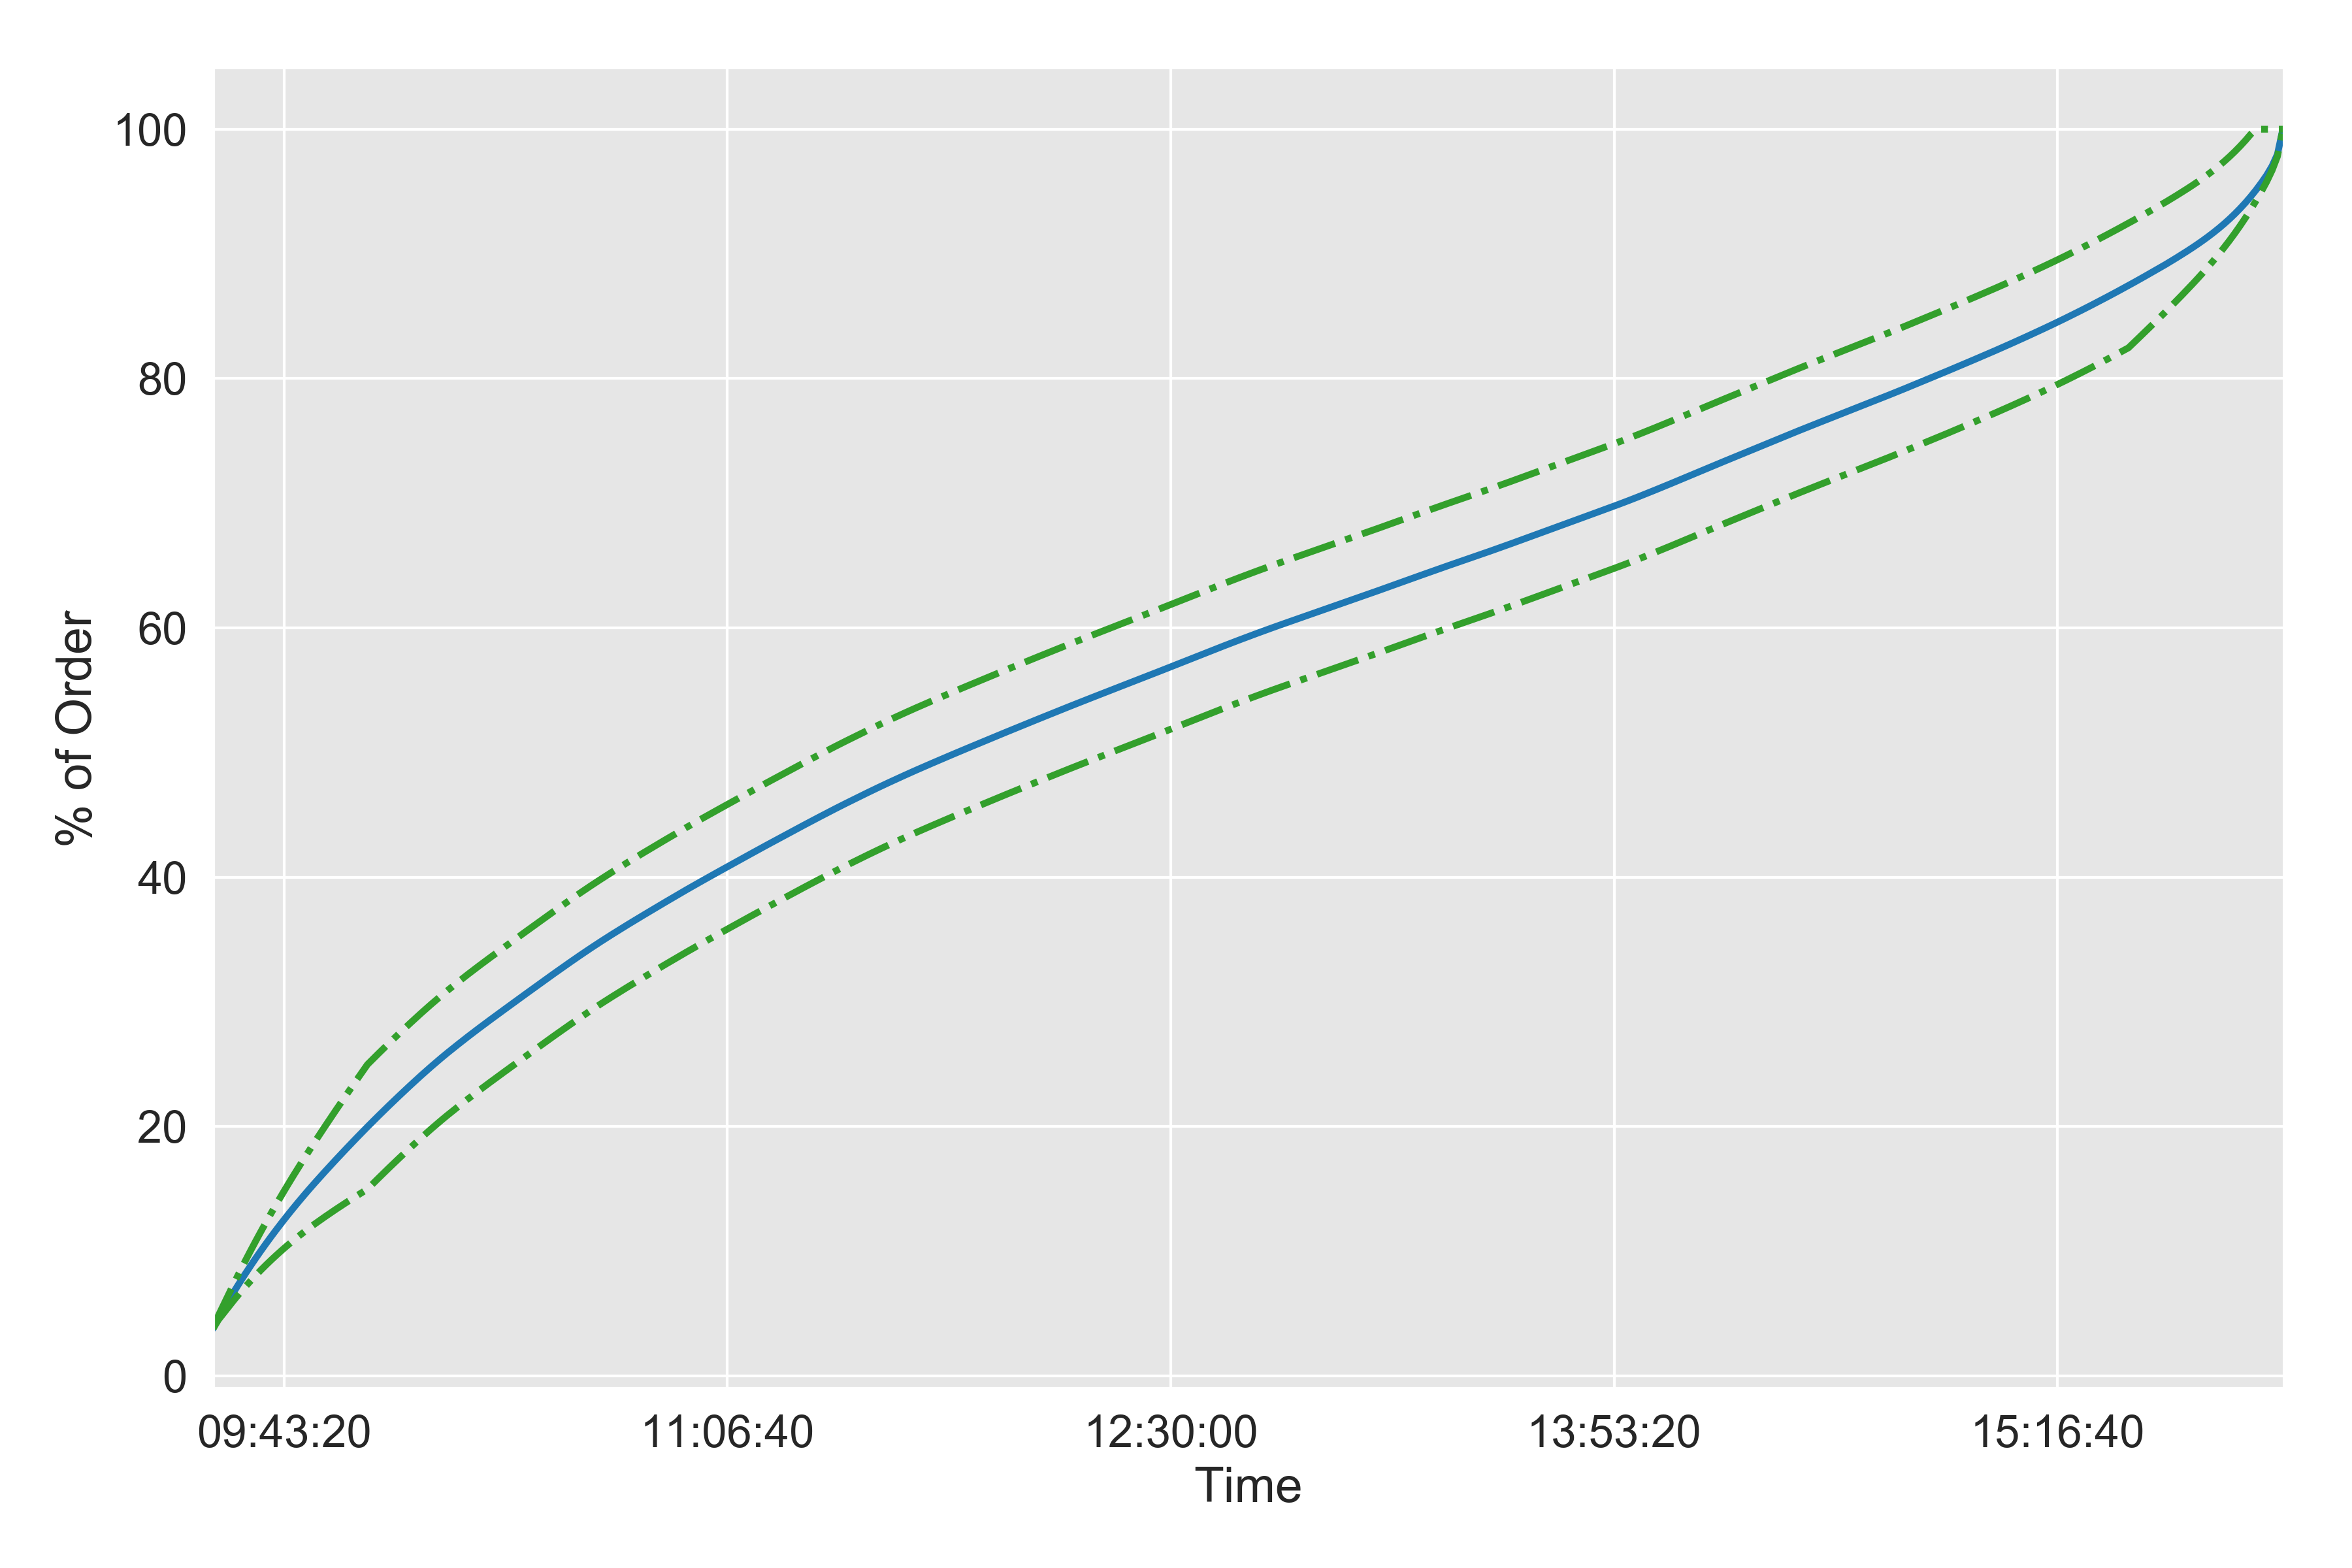
\includegraphics[width=\textwidth]{chapters/chapter_exec_models/figures/schedule.png} 
	\caption{Example VWAP schedule with bands. \label{fig:schedule}}
	\end{figure}

Using the trading bands the scheduler will determine if and how much it needs to catch up to the schedule so as not to fall too much behind or in general end up with the risk of catch-up.\footnote{It is well known that arbitrary, unconditional, catch-up is one of the significant drags in performance. Additionally many traders are extremely risk averse and will tend to cancel an order that is too far behind schedule.} The scheduler will then determine how much shortfall it needs to make up and the opportunistic quantity it has available since it is allowed to be ahead of schedule. It can then pass these minimum and maximum quantities to the order placement so that it can be more nuanced around how to manage the required trading needs. Figure~\ref{fig:sch_details} gives a visual representation of the information set available to a general scheduler.

	\begin{figure}[!ht]
	\centering
	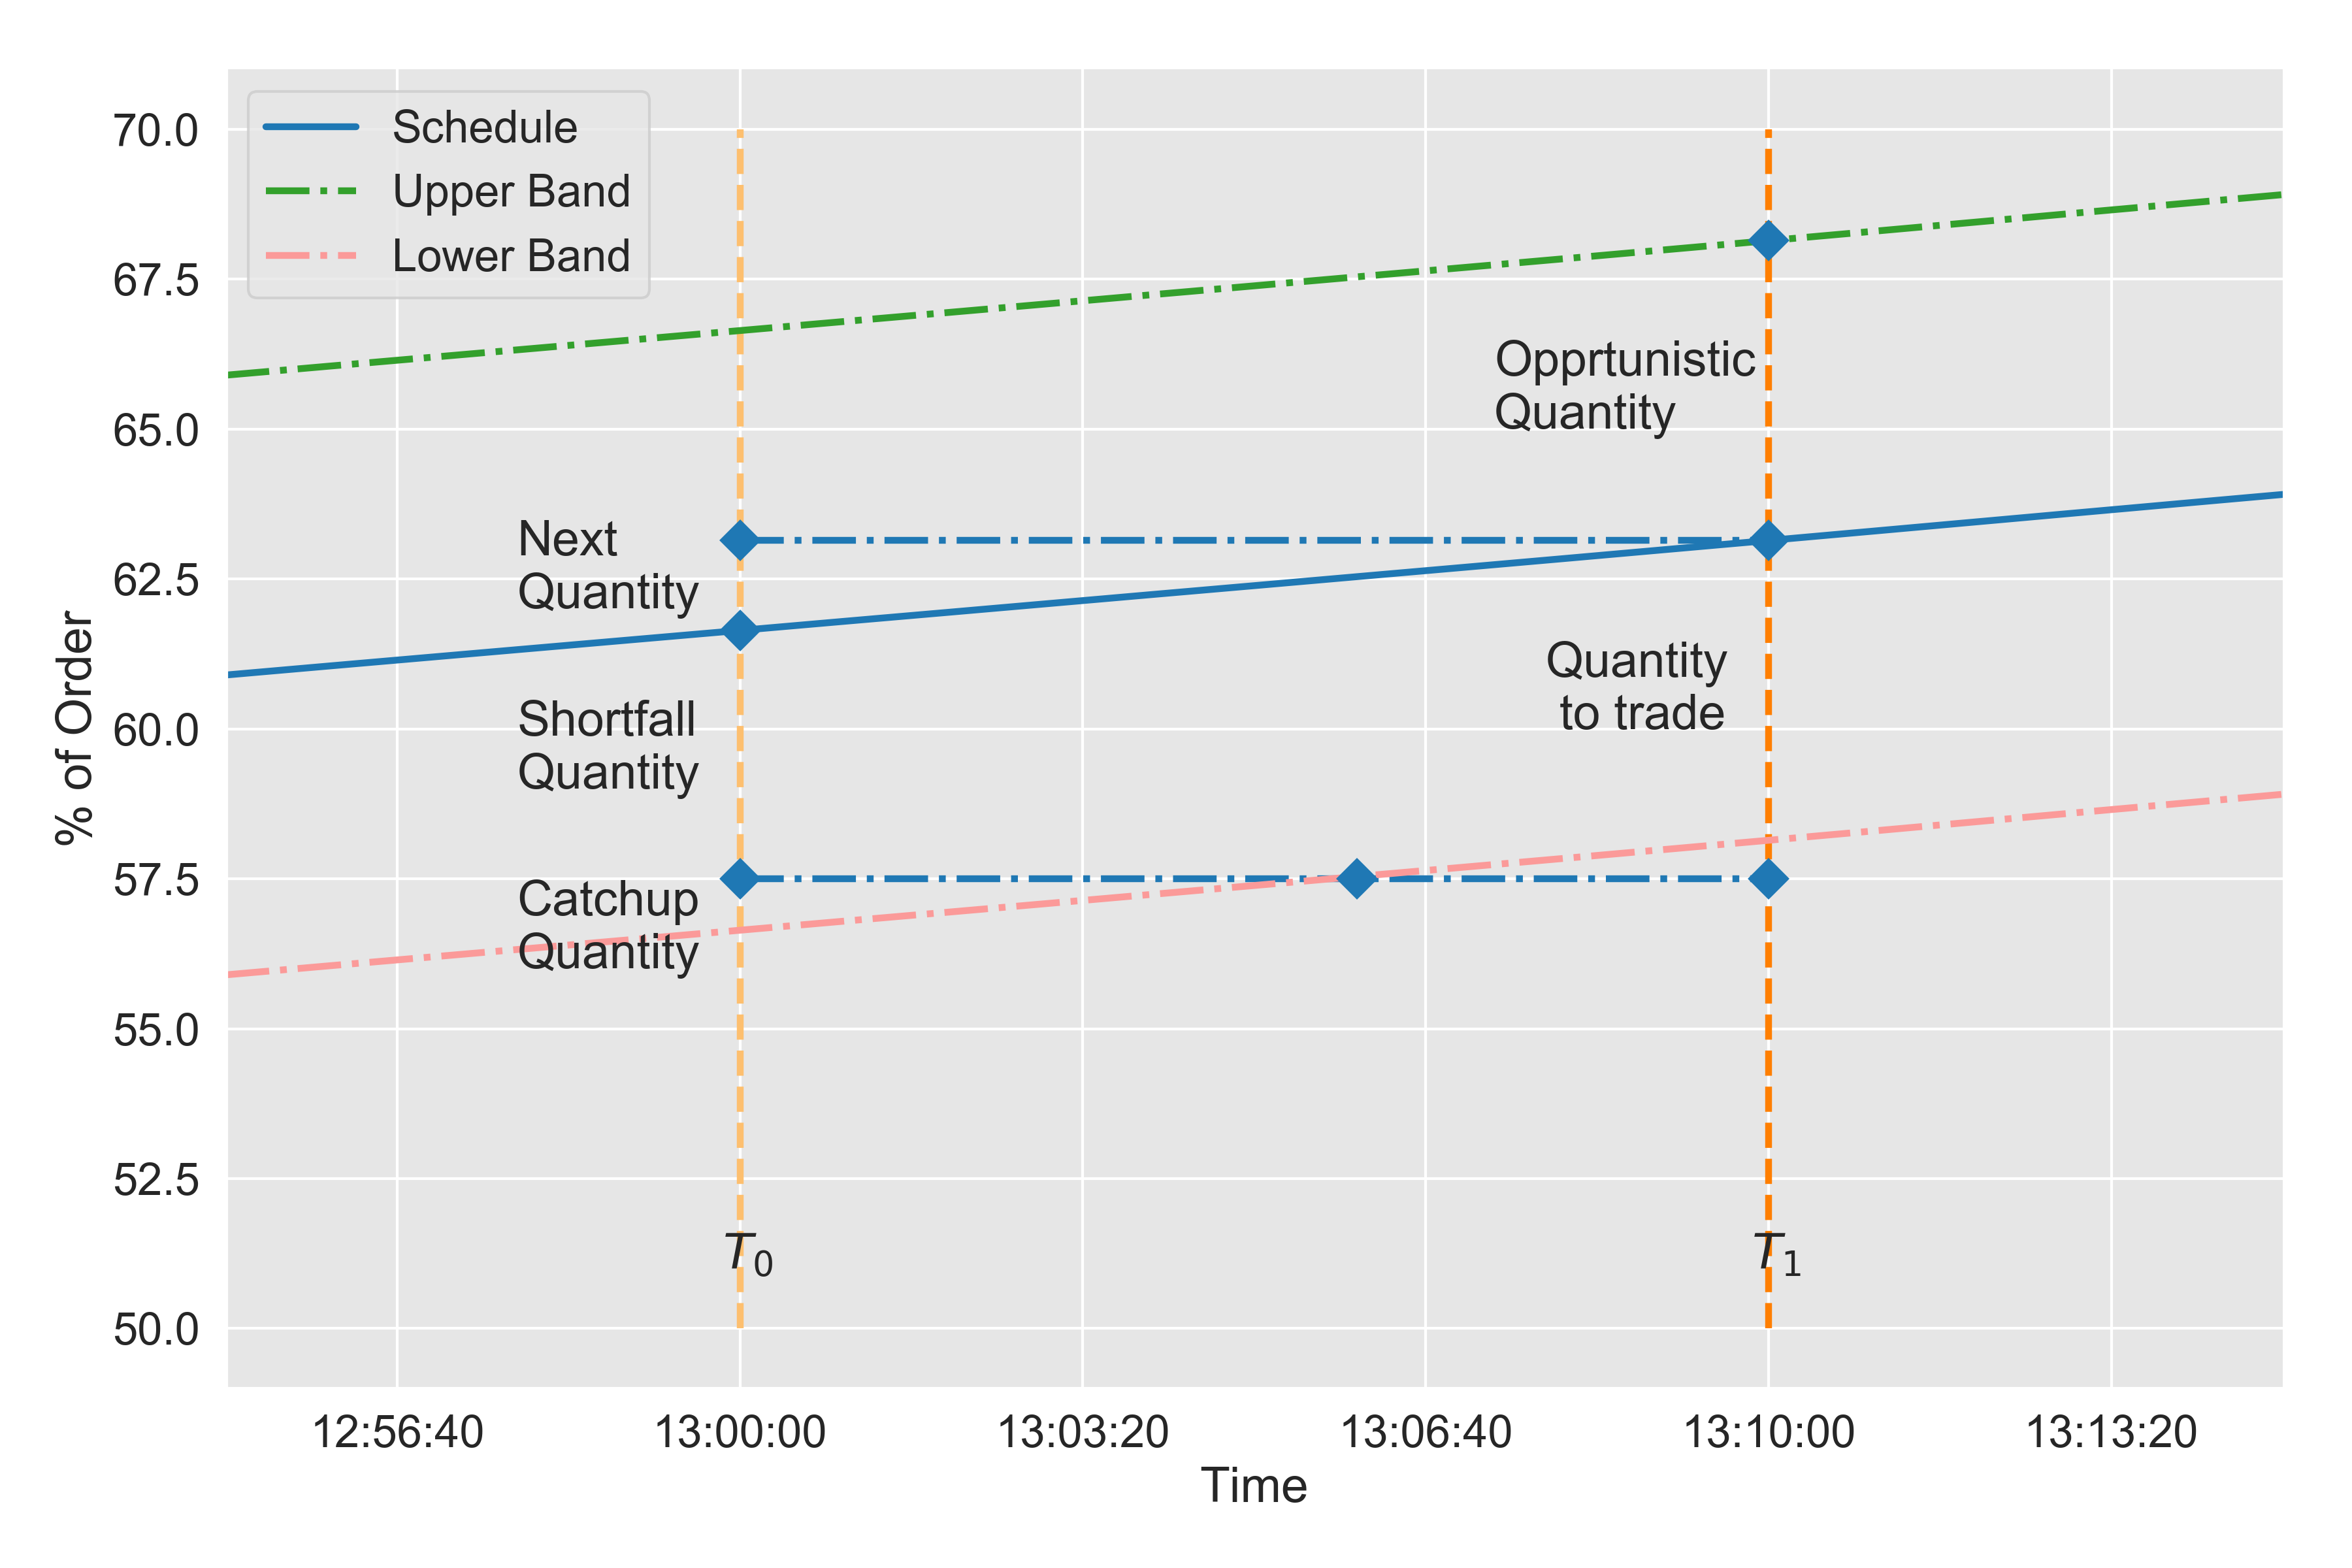
\includegraphics[width=\textwidth]{chapters/chapter_exec_models/figures/schedule_details.png} 
	\caption{Schedule information set. \label{fig:sch_details}}
	\end{figure}

At the beginning of every time bin, the strategy will asses four main state variables:

\begin{enumerate}
\item\emph{Target Quantity}: this is where the strategy should be at at time $t_0$ ( point A )
\item\emph{Current Quantity}: this is where the strategy is (point B)
\item\emph{Next Quantity}: this is where the strategy should be a time $t_1$ (point C)
\item\emph{Opportunistic Quantity}: this is where the maximum quantity strategy can be be a time $t_1$ (point D)
\end{enumerate}


One other important consideration is at what time, if no trading happens will the strategy hit the lower band and thus will need to catch up (point L). The difference between the Target Quantity and the other points provide with the necessary  information for the strategy to decide the instructions to the order placement layer to maximize the chances to execute the required shares to stay on schedule and how much leeway it has to stay behind or can be ahead. By providing the order placement with a quantity range has the additional benefit that it allows the execution to be ahead of schedule when conditions are favorable leading to reduced catch-up behavior and thus resulting in reduced impact and improved performance.


The distance between the bands and the schedule can be made more stock specific allowing to further refine the behavior across the trading universe. It can also made to be client specific as it represents the traders risk aversion from schedule deviation. The wider the bands the less risk of unilateral catch-up but the larger the risk of significant deviation from the desired schedule. \twomedskip


\noindent\emph{Stateless Approach}: An improved approach to this is for the strategy to not use time bins at all but work in a more stateless fashion. The scheduler re-evaluates the same state variables on a continuous basis (every few seconds for example) and adjusts the instructions to the order placement by a small amount each time to refine the trading policy. The schedule can also use several points in the future to provide more term structure to the policy and thus plan better ahead, in particular when the schedule start having significant ``curvature'' for example at the end of the order. \twomedskip


\noindent\emph{Systematic Deviation}: A final improvement to this approach, we will briefly discuss is the usage of predictive signals (aka alpha) within the schedule. If one has a prediction of short term price move it can leverage that by making a systematic decision to get ahead or stay behind schedule in order to take advantage of that price information. This has to be done carefully to avoid incurring in any additional market impact or risk of catch-up that will cancel out any possible benefit of this move. The schedule also needs to have a component that will encourage the strategy to get back on schedule if the price prediction subsides. This will avoid the strategy to remain ahead(behind) for longer than necessary incurring in unnecessary schedule risk.



% Order Placement
\subsection{Order Placement}

The order placement layer sits downstream from the scheduling layer and can be seen as the micro trader of the strategy. It is in charge of decisions spanning the upcoming few seconds or minutes of trading. In general this layer is unaware of the overall trading intention received by the scheduler and it is responsible for implementing locally its decisions. More sophisticated approach might leverage  additional instructions from the scheduler providing a picture on the macro state of the order in  order to nuance the decision making. In any case, we can simplify the role of the micro trader as answering the question: ``at what price should I trade the quantity allocated for the upcoming period in order to complete and obtain the best possible price?'' 


How does one approach this problem? Let us follow the historical evolution of Order Placement techniques to explore the various challenges and possible solutions. \twomedskip


\noindent\emph{Na\"ive Order Placement}: The simplest approach possible would be to send the given quantity as a market order and completely fill its allocated quantity immediately with essentially no uncertainty in the outcome. A view of the aggregated order-book will provide a very good, conservative (because it does not include the possibility of mid-point hidden orders), expectation of what average price would be achieved. Depending on the characteristics of the order and the stock it is trading the size to trade might still be larger than what can be absorbed by the market without ``eating'' into the order-book. This could be simply remedied by decreasing the schedule interval.


The first order placement modules were not that much different than this na\"ive approach. While for highly liquid instruments with tight spread, this approach might achieve decent results but as we go down the spectrum of liquidity, things start falling apart and one will need to introduce the additional complexity that comes with leveraging non-marketable orders. \twomedskip


\noindent\emph{Peg and Cross:} The next step in the evolution of order placement approaches is often termed ``Peg and Cross''. It consists of placing a limit order  for the scheduled quantity at the near side. If the market moves away the order can be repriced (alternatively one can rely on a peg order type to do this) and size updated if necessary. If the order is not fully executed by the time the schedule reaches the catch-up zone an aggressive order is sent to get back on schedule.


Variations of this approach are still the norm in many product implementations across the industry. One advantage of the approach is that if  the order is executed passively on a maker-taker exchange it will earn a rebate which makes the overall cost of trading lower. On the downside this technique will consistently be adversely selected with most of the passive executions happening when the price is ``coming through'' and will often be more attractive right after the order is filled.


One approach to minimize this adverse selection is to ``layer'' the order book with some of the available quantity so as to capture execution at better price levels when the price comes through. Ideally, if the infrastructure is fast enough and one uses some short term signals like order imbalance to predict when the probability of price drop reaches a critical threshold is to cancel the top order so as to further minimize the adverse selection. This is a common approach of HFTs where they want to be at the top of the book to capture a fill right before the price moves away.


A common variant of the Peg and Cross technique is to leverage additional price points, in particular the mod point. As the need for liquidity increases the order placement can either ping the mid of various exchanges or have a quantity hidden at the midpoint to increase the probability of getting filled. \twomedskip


\noindent\emph{Beyond Peg and Cross:} More sophisticated approaches are possible and are used in some advanced implementations. These models are quite proprietary and the authors do not pretend to have seen them all. We will just give a few additional pointers.


One direction in which these models evolved is to leverage Reinforcement Learning techniques. These models are notoriously hard to calibrate and require a good order book simulation environment. They are also limited in scope as most simulators require what is called a ``small order'' assumption meaning that the quantity traded does not meaningfully alter the state of the market and thus does not require to inject strong assumption in the simulator on how the market will react. This is definitively an interesting space of research that could lead to valuable breakthroughs in the future.


Other approaches use more heuristic methods around liquidity interaction but leverage more nuanced systematic approach to experiment the optimal usage of different heuristics. There is more focus on speed, low latency and alpha signal utilization to trade aggressively when the price is ready to move away and ``stepping out'' of the way when the market is about to come through.


One particular area for obvious improvement is the tendency for a one-size-fits-all approach to order placement meaning that, apart the usual normalization practices, the approach is uniform across the stock universe. This is an area that clearly can be substantially improved upon. For example, there is a subset of instruments with very volatile and thin order books where posting liquidity does not really add any value and could benefit from a more opportunistic approach. Stocks withe ultra-long queues could use different methods to maintain ``density'' within the order book and canceling orders when no liquidity is needed.


Finally, low liquidity stocks likely require a complete new approach and will be an area of focus in particular for generally illiquid markets in Europe and APAC and has the investment expands to the lower liquidity instruments. There is so much more that can be said around this topic but we hope that this brief treatment provides enough meat for the interested reader to explore this exiting space.



% Order Routing
\subsection{Order Routing}

The output of the order placement layer can be modeled as an array of price levels and associated quantity such as $[ [18.85 ; 600], [18.84 ; 400], [18.81 ; 200] ]$ that is then passed on to the order router for execution or quoting on the market.


The order routing layer sits downstream from the order placement layer and is in charge of the ultra high-frequency decisions (of the order of microseconds to milliseconds). Given the volume and complexity of events to process in a fragmented market environment and the sensitivity to latency, the routing decisions are often delegated to the Smart Order Router (SOR) rather than handled by the algorithmic strategy itself. While it is also generally unaware of the overall trading intention received by the scheduler, it is responsible for implementing the decisions of the order placement module. As such, the SOR answers the question ``to which exchange(s) should I route the child order in order to maximize the probability of getting a fill at or better than the desired price?'' This component is of particular importance in fragmented markets, and might be absent in execution strategies interacting with single markets (EM Equities, Futures, etc.). 


While probably the simplest component of the execution stack from a quantitative point of view, the SOR implements rather complex decisions to achieve several objectives: 

\begin{itemize}
\item \textbf{Sourcing liquidity efficiently:} This is the primary objective of the component in charge of handling the fragmentation complexity, but it takes different forms as a function of the instructions received from the order placement module. For passive orders, sourcing liquidity efficiently means maximizing the probably of fill and minimizing the time to fill. For aggressive orders, this means maximizing the fill rate.

\item \textbf{Optimizing price:} The instructions received by the SOR are in the form of a limit order and a Time-in-Force. For Immediate or Cancel order (IOC) instructions intending to remove liquidity from the order book, the limit price is a maximum (minimum) for a buy (sell) order, giving the router the optionality to eventually find a better price and provide price improvement to the order placement module.

\item \textbf{Managing execution fees:} Venues have various pricing models (flat price, maker-taker, taker-maker) and charge different prices to access their liquidity. Thus, the SOR can optimize routing in order to minimize fees (or maximize rebates), at the potential expense of lower fill rates.
\end{itemize}


In practice, these objectives are somewhat contradictory and have to be assigned different weights to reflect the traders' preferences with respect to the implicit tradeoff they represent. There are also a common set of factors that directly influence routing decisions:


\begin{itemize}
\item Relative price target of the child order: near touch, far touch or mid point. This is the first and main input influencing routing decisions. The handling of the other features described below will first depend on the price being targeted.

\item Algo parent order urgency or liquidity demand: low urgency parent order algorithms target low percentage of volume over the course of the execution as a result of low risk aversion or low perceived alpha. As a consequence, they do not need to access all available liquidity at all points in time and can focus on quality over quantity. Conversely, high urgency algo strategies are used by traders with fast-realizing alpha and favor liquidity extraction over quality considerations.

\item Algo child order urgency: irrespective of the longer scale urgency of the algorithm, child orders also have different degrees of urgencies depending on the reason why they were generated. Passive orders are associated with a horizon by the end of which they are expected to be filled. The longer the horizon, the deeper in the book they can be posted. Aggressive orders also have varying degrees of urgency, from low urgency if the algorithm is crossing the spread to maintain a target execution schedule (for instance after hitting the lower band surrounding the schedule due to insufficient passive fills), to high urgency if the algorithm is crossing the spread due to a trading signal indicating a short lived opportunity to capture advantageous liquidity (being due to its size or price).

\item Child order size: for aggressive orders, the relative size of the child order compared to the available far touch size also offers some optionality. If the order is small compared to the available liquidity, the SOR can search for price improvement opportunities without being too exposed to the opportunity cost resulting from far touch orders cancellation. Conversely, oversized orders require fast routing in order to maximize fill rate before the liquidity fades away.

\item Intended liquidity destination: lit or dark markets.

\item Execution cost: venue specific cost can also vary for aggressive and passive orders, and some strategies might explicitly target a maximum execution cost to remain profitable. \twomedskip
\end{itemize}


\noindent\textbf{Implementing a Smart Order Router:} \twomedskip


The role of smart order router being to handle the liquidity fragmentation in a HFT landscape, the first consideration that comes in the implementation of a SOR is speed. This is a requirement for the processing of both order instructions and inbound market data used to make these routing decisions. A modern SOR is expected to receive direct feeds from the exchanges it connects to and process that market data to reconstruct the composite order book in as near real time as possible, which in many cases is achieved with hardware based solutions rather than software. From an implementation point of view, for time sensitive decisions, the optimal behavior is generally modeled offline and then stored as a collection of routing tables that allow the SOR to swiftly implement the desired routing sequences based on the top level algorithm characteristics and its local intent. For passive orders, targeting the near touch or mid point, the SOR can afford to solve the problem online in order to determine optimal allocation across eligible venues. 


As described above, the objectives of the router differ across orders and over time, taking into consideration multi-dimensional features, and resulting in a large number of scenarios. For illustration purposes, we will provide a few examples of the opportunities and challenges the SOR faces for different target price points. 


\begin{itemize}
\item \textbf{Near side orders:} When submitting passive orders, the main objective is to optimize queue position in order to maximize the probability of obtaining a fill\footnote{The SOR can be either cost-agnostic and favor fill rates and time to fill, or cost-aware and try to maximize rebates in markets that have a maker-taker pricing model. This would, obviously, result in different routing strategies.} before the market moves away, while competing with the other liquidity providers. There are a few factors that directly influence the fill probability of orders routed to the near side:


\begin{itemize}
\item Price: the closer to the top of book, the higher the probability of fill, and lower expected time to fill, everything else being equal.

\item Queue length: long queue names, in particular when price volatility is low, exhibit significant queue position competition on the passive side, resulting in longer time to fill and generally lower probability of fill. This decrease in fill probability is more pronounced at deeper levels in the book as these names barely trade beyond the touch. 

\item Resting time: the longer an order rests in the order book, the higher its fill probability as it progressively accrues queue priority in price-time order books following other executions and order cancellations.

\item Size: smaller orders (with respect to the available liquidity) tend to enjoy higher fill rates than their oversized counterparts.
\end{itemize}


In a fragmented market, these factors have different values on each venue giving the router an opportunity to dynamically optimize liquidity sourcing as volume shifts from exchange to exchange. This is an essential part of achieving best execution as na\"ively  sending a passive child order to a venue and resting it there for a period of time without getting any execution while transactions happen in other venues might incur opportunity cost if the market moves away and the child order ends up being traded at a less favorable price later on. \twomedskip


Na\"ive posting strategies allocate shares evenly across venues, or proportionally to each venue's market share. Other utilize simple routing tables where venues are ranked in decreasing order of preference (based on market share or fees) and shares allocated sequentially up to an allowable quantity before moving on to the next venue. More quantitative routing decisions for lit passive posting can be expressed as a constrained optimization problem: given $X$ shares to execute, $[n_1, n_2, \ldots, n_Y]$ shares displayed on the book of lit venues $[1, 2, \ldots, Y]$ and some expected trading rates at each venue $[v_1, v_2, \ldots, v_Y]$ over the desired execution horizon, what is the combination of shares sent to different venues that maximizes the overall fill probability and minimizes time to fill? Some recent academic research in this area is discussed in Section~\ref{sec:mult_exch_sora}.


\item \textbf{Mid-point orders:} For these orders, the destination is usually dark pools, which present different inherent challenges. While lit executions and order books are public and can be observed in market data feeds, dark order books are invisible (making it difficult to estimate the fill probability a priori at the time of routing) and dark executions tend to be reported in aggregate (for instance, under a single condition code), thus making attribution of actual execution venue more challenging. In this context, if solely observed from market data, dark executions in the US cannot be directly attributed to one of the numerous non-displayed venues. However, if observed from the point of view of an executing entity (through execution fills received), one is in possession of censored observations of the available---otherwise invisible---liquidity (i.e. when receiving a fill for $X$ shares one knows there were at least $X$ shares available to trade on the other side in this particular venue and can use this information as an input to the next round of decisions). 


Additionally, dark venues are not all made equal, and the quality of their liquidity is usually assessed by practitioners as a function of: 

\begin{itemize}
\item Average order size: the larger, the better as it tends to indicate the presence of natural liquidity that most execution algorithms favor interacting with.

\item Uniqueness: there is no precise rule here, but a fill can be considered unique if there is no other dark trade happening on the same symbol in the moments immediately preceding and following the print. More unique prints are also generally indicative of the presence of natural liquidity as market makers (considered to be non-natural liquidity) tend to quote in multiple venues at once.

\item Short term reversion: measured as the trajectory of the mid point immediately following an execution (usually at time-frames ranging from a few milliseconds to a few seconds). Large, adverse, moves are often an indication of a certain toxicity of the venue. 
\end{itemize}


These metrics directly influence routing decisions. While a venue might be executing large quantities, the quality of its liquidity might not always make it a desirable destination for all types of executions. For low urgency executions (low participation rate, low expected alpha), the router can afford to be more restrictive in the venues it accesses, focusing on venues with larger---more unique---liquidity; while for high urgency orders (demanding both large liquidity and immediacy due to superior alpha), it might be setup to access all venues in order to maximize liquidity extraction.


Here too, na\"ive posting strategies allocate shares either evenly across venues, or they utilize simple routing tables where venues are ranked in decreasing order of market share and shares are allocated sequentially up to an allowable quantity before moving on to the next venue. For aggressive order intending to sweep dark pools quickly before performing another action, the main consideration is usually speed, as a result of which the number of venues explored tend to be more limited. Aggressive dark sweep tactics favor venues that are close in space (and time) and have the fastest matching engines to minimize the opportunity cost associated with the round trip time necessary to receive a fill or an IOC cancellation back. From a quantitative perspective, given the transient nature of dark liquidity and the inherent uncertainty, dark allocation is a classic multi-armed bandit problem: given $X$ shares to execute and $Y$ available venues with unknown available liquidity and unknown trading rates, what is the combination of shares sent to different venues that maximizes the fill probability and minimizes the time to fill? The exploration versus exploitation dilemma favors incurring some opportunity cost by allocating shares to venues with low probability of execution in order to obtain information about the potential presence of liquidity there at a particular point in time.


\item \textbf{Far side orders:} For these orders, maximizing fill rate is the primary objective, followed by obtaining price improvement if the child order is not particularly urgent. The main challenge for aggressive take orders is to be able to capture all the liquidity that was visible at the time the child order is initiated. Market participants, in particular high frequency market makers, tend to display liquidity on multiple venues simultaneously and are likely to attempt to cancel all other outstanding child orders once they receive the execution confirmation from the first venue to get hit in order to avoid adverse selection, thereby depriving the aggressive trader of capturing all the intended liquidity that was displayed.\footnote{This is possible due to the latency that exists when sending orders to multiple, physically distant, exchanges.} Market makers may then replace their quotes deeper in the order book as a reflection of their temporary lesser appetite for additional inventory. Hence, the trading algorithm attempting to capture all visible liquidity on the far touch at a point in time might end up getting only a partial execution and may have to trade the remainder of the slice at a less favorable price. This rapid vanishing of liquidity immediately following a trade is known as a ``fading'' effect and can be particularly costly over time for liquidity takers who might need to pay extra ticks to access the amount of volume they need at a point in time. To guard against such fading, SORs are borrowing from the military repertoire and implement Time-on-Target coordination tactics.\footnote{Time-on-Target is a military term used to describe the coordinated firing or artillery by many weapons so that all munitions hit the target at the same time.} Most advanced SORs incorporate estimations of the (time) distance separating them from the matching engines of these venues in order to optimize child order routing sequence so that all routed orders hit the various exchanges at approximately the same time. Another common tactic employed consists in firing first the largest orders so that the potential fading faced by later orders has less impact from a total fill rate perspective. 

When the urgency of the child order is not high, for instance if the objective of the aggressive order is just to catch-up to a prescribed schedule with a low-frequency granularity (of the order of minutes), then the routing is not really time sensitive and can also leverage the SOR ability to access both lit and dark venues. Even if the original order was intended to trade on a lit market, the low urgency of the desired action gives the SOR the opportunity to try to source mid point liquidity first --- to get some price improvement --- before completing the intended action with the residual quantity. This technique is generally described as ``dark pinging'' and sequentially scans a set of dark pools prior to performing low urgency spread crossing. The selection of which pools to scan through follows a similar approach as orders intended for mid point routing in the previous paragraph: the tradeoff between quantity and quality depends on the urgency of the overall order.
\end{itemize}


Similarly to the top level trading algorithm, the end users evaluate the performance of the SOR using metrics aimed at measuring the performance of liquidity sourcing such as analyzing fill rate on aggressive limit orders (higher fill rate meaning a more efficient routing less subject to fading), the ratio of routed versus executed quantity, and average time to fill on passive orders (less unsuccessful routing and shorter time to fill meaning less potential opportunity cost incurred by child orders due to inefficient routing).



% Review of academic treatment of Execution Strategies
\section{Mathematical Description of Execution Models}


As discussed in the last sections, while algorithmic trading techniques are useful in both low and high frequency settings, their importance has become more pronounced in the age of electronic trading because of the speed in execution and the necessity for efficient matching of demand and supply sides in the limit order book. Added to this is that modern equity markets where order submission and cancellations are automated and are also highly fragmented with dozens of exchanges and about forty alternative trading systems where investors can choose to trade. The trading algorithms also differ over various types of market participants, but all of them have common objectives, that is to optimize dynamically where, how often and at what price to trade. The algorithms have small reaction times to changing liquidity and price. Typically, to summarize the execution has been broadly classified into the following layers.
	\begin{itemize}
	\item \textbf{Scheduler (Macro Level):} Given a meta-order (parent trade) translate the objective function of a strategy into a trading schedule; when the algorithm should trade, in what size (child order), for how long and the spread of trading.
	
	\item \textbf{Order Placement (Micro Level):} Given a slice (child order) of the meta-order to trade, this layer of algorithm decides whether to place it as a market or as a  limit order and at what price level.
	
	\item \textbf{Order Routing (Smart Order Router):} For a given order (quantity and price level) to which venue should the order be sent. This part covers the so-called space dimension.
	\end{itemize}


In this section, we discuss methods involved in these and other execution issues in the high frequency trading context. Generally, as indicated earlier, the objectives of equity trading are to minimize the probability of making errors---minimizing the trading impact and avoiding adverse selection. In order to achieve high completion rates, the trading should operate with speed and necessary risk control. It has to be noted that the average trade size is empirically shown to have come down over time; thus the parent orders are increasingly decimated and are sent to the exchanges as small child orders. Handling this with large parent order sizes with the focus on short-term alphas requires a great deal of trade timing insights as discussed before.


The execution agencies engage in providing pre-trade advice and post-trade reporting. The pre-trade advice includes the estimation of market impact cost covered in Chapter~\ref{chap:ch_mi_models} and the post-trade reporting is useful for evaluating how well the agency's execution algorithm has performed as compared to some benchmarks. Some of these include the fill rate, the fill composition (passive values aggressive covering the spread) and the evaluation measures such as the magnitude of price revision against the order after the trading ends. Different clients are likely to put different emphasis on these measures. 


These algorithms have been generated over time and they follow closely how the complexity in trading has grown. The first generation algorithms focus on trading at fixed rate over a time-aggregated interval, trading at a fixed participation rate and trading such that the average execution price is closer to market volume-weighted average price which were described at length earlier. The second generation algorithms focus on market impact and risk. The methods here are formalized similar to Markowitz's portfolio theory. Increasing risk aversion generally leads to shorter execution with higher market impact. As more trades occur near the market close, risk averse clients may trade entirely at the closing auction. Finally, the third generation algorithms closely track the state of the limit order book and market data and are adaptive. The optimal decision such as updating the limit price, crossing the spread, cancellation of orders result from stochastic control formulation. The basic data used in these algorithms follow from microstructure signals covered in Chapter~\ref{chap:ch_trade_data_models}. 


% Execution Algorithms: Some Preliminaries
\subsection{Some Preliminaries}

The primary goal of most of the execution algorithms is to minimize the transaction costs which are broadly divided into direct costs and into indirect costs. The direct costs such as commissions, taxes etc are easy to measure and they primarily depend on quantity of trading. The indirect costs such as market impact and opportunity costs are hard to measure and depend upon trading strategies. Because many mutual fund and hedge fund companies engage in portfolio rebalancing periodically, they trade a large block of shares in a fixed duration. There is a trade-off between trading a large market order that is likely to affect the price adversely and splitting the parent order into many child orders and let the market recover after each trade. The modeling elements generally involve representing the permanent impact of a parent order, the temporary impact of trading a child order (when the price normally returns back to equilibrium short time after the trade) drift in price (alpha) and the volatility of the stock. The optimizing function balances the cost-loss in revenue due to price impact and the risk-uncertainty due to volatility of the underlying stock. If the trade occurs fast, we incur high cost and low risk but if the trade occurs slowly, we incur low cost and high risk.


The execution algorithms are generally evaluated through some benchmark prices. Some key quantities are:
	\begin{enumerate}[--]
	\item Arrival price, that is the market mid-quote at the start of parent order execution at $t= 0$, $p_0$.
	\item Volume weighted average market price over the period of execution, $t \in (0,T)$, $p_{\text{VWAP}}= \sum_{i=1}^N v_ip_i/v$ (Equation~\ref{eq:vwapstet}). \twomedskip
	If the parent order of size, $X$ is split into `$n$' child orders with size, $x_k$, $k=1,\ldots,n$, then
	\item Volume weighted average price of the parent order's execution, $p_{\text{exec}}= \sum_{i=1}^n x_ip_i/X$. 
	\end{enumerate}
	
Two other related quantities that the traders examine in their evaluation strategies are as discussed earlier:
	\begin{enumerate}[--]
	\item Slippage: $s= p_{\text{bench}} - p_{\text{exec}}$
	\item Market Impact: $p_0 - p_{\text{VWAP}}$
	\end{enumerate}
The execution cost is taken to be the slippage and the execution risk is its standard deviation. 


The influential paper by Kyle (1985)~\cite{kyle1985} argues that traders split the parent order to hide private information. The splitting of the order and how they are sent to the market, the strategies depend on the evolution of the stock price. These are broadly classified into static, one determined in advance of trading and into dynamic, one that depends on the state of the market. The static strategy under some conditions can also be dynamically optimal. Few commonly used criteria for allocation strategies are:
	\[
	\begin{split}
	&\text{VWAP: } x_k= X \cdot \dfrac{V_k}{V} \\
	&\text{Percentage of Volume: Minimize } \left( \dfrac{\text{Volume}_{\text{exec}}(x_k)}{\text{Volume}_{\text{market}}(v_k)} - v_{\text{target}} \right). \\
	&\text{Implementation Shortfall with risk: Minimize } E(s) + \lambda \var(s)
	\end{split}
	\]
These strategies as stated are static and they are based on a priori models for the evolution of price and volume traded over different times of the day. 


We present below select results in this area. The quantities that the trader can determine are the number of child orders $(n)$ and their sizes $(x_k)$ and the duration for the parent order trading $(T)$. The relevance of this problem to the practitioners is also discussed in Chan and Lakonishok (1997)~\cite{lakon} and Keim and Madhavan (1997)~\cite{madhavan}. Bestimas and Lo (1998)~\cite{berlo} develop a model that suggests splitting the parent order to reduce the average trading costs. Almgren and Chriss (2000)~\cite{alm2000} split the parent order to minimize the mean-variance of trading costs (implementation shortfall with risk) similar to Markowitz's portfolio theorem. Some recent works on this topic are also briefly mentioned but, described in some detail in the following sections.


% First Generation Algorithms
\subsection{First Generation Algorithms \label{sec:first_gen}}

The performance of traders is evaluated by how they execute the orders in comparison to volume weighted average price (VWAP), because it is generally considered to be closer to how a passive trader would trade. Madhavan (2002)~\cite{mad_a02} warns that the uncritical use of VWAP as a benchmark can promote non-optimal trading behavior. The choice of a benchmark will obviously affect the placement strategies by the traders. Recall the discussion earlier how traders are shifting the orders toward the market close as large numbers of trades occur during the closing hour. Using daily VWAP as a benchmark leads to trades spread over the day and thus passive trading can significantly affect alpha. The pre-trade benchmarks such as the arrival price ignore the short-term trends in prices. The post-trade benchmarks are sensitive to order flows towards the end of the day and thus have higher price impact. The VWAP strategy can be automated so that order submissions can follow historical volume pattern during the course of the day with finer time grids. This practical approach is expounded in this section.


We will follow the formulation of the optimization problem as given in Busseti and Boyd (2015)~\cite{busseli_boyd}. With $X$, the total number of shares to be traded over the time horizon, $(0,T)$ in `$n$' discrete time intervals, the problem is to decide how to divide the parent order $X$ into child orders $x_1, \ldots, x_n$ so that the executed average price $p_{\text{exec}}$ is closer to $p_{\text{VWAP}}$. It is assumed that the price, $p_t$, is a random walk and thus the return is white noise. It is assumed that the trading algorithm mixes optimally market and limit orders. Defining the cost of trade in time interval $t$ as $x_t \hat{p}_t$, where $\hat{p}_t$ is the effective price that depends on the instantaneous transaction costs such as bid-ask spread with `$s_t$' as the fractional bid-ask spread with a certain participation rate $x_t/v_t$, it can be shown that the effective price is
	\begin{equation}
	\hat{p}_t= p_t \left(1 - \dfrac{s_t}{2} + \alpha \, \dfrac{s_t}{2} \cdot \dfrac{x_t}{v_t} \right),
	\end{equation}
which gives in the end quadratic transaction costs which is a reasonable approximation as seen from Chapter~\ref{chap:ch_trade_data_models}. Here `$\alpha$' is taken to be proportionally factor of market orders to total orders. Defining the proportional ratio
	\begin{equation}
	s= \dfrac{X p_{\text{VWAP}} - \sum x_t \hat{p}_t}{X p_{\text{VWAP}}}
	\end{equation}
as slippage, where the numerator is the cash flow to the broker, the optimizing function is
	\begin{equation} \label{eq:opt_function}
	E(s) + \lambda \var(s).
	\end{equation}
Here `$\lambda$' is the risk-aversion parameter. It has to be kept in mind that the quantities $p_t$ and $v_t$ are random variables and the decision variable is `$x_t$'. Note with some approximation, $p_t \sim p_{t-1} \sim p_{\text{VWAP}}$ and with applying the law of iterated expectation, the optimization in \eqref{eq:opt_function} simplifies to
	\begin{equation}
	\min_{x_t} \sum_{t=1}^n \left[ \dfrac{s_t}{2x} (\alpha x_t^2 k_t - x_t) + \lambda \sigma_t^2 \left( \left( \sum_{r=1}^t u_r/X \right)^2 - 2 M_t \sum_{r=1}^{t-1} u_t \right) \right]
	\end{equation}
with constraints $x_t \geq 0$ and $\sum_{t=1}^n x_t = X$. Here the quantities $M_t= E \left[ \sum_{r=1}^{t-1} v_t/v\right]$ and $k_t= E[\frac{1}{v_t}]$ refer to market intra-day volume distribution. Assuming that the spread is a constant which is generally true for actively traded stocks, the optimal static solution can be shown to be equal to:
	\begin{equation} \label{eq:optimal_result_xt}
	x_t^*= X E\left(\dfrac{v_t}{v}\right), \enskip\enskip t=1,\ldots,n.
	\end{equation}
From the above discussion, it is clear that forecasting both the intra-day distribution of periodic volume, $v_t$, and the total volume for the day, $v$, is essential for achieving optimal results. The optimal result in \eqref{eq:optimal_result_xt} can be obtained also with slippage as defined in the previous section. \twomedskip


\noindent\textbf{Bertsimas and Lo Model:} The basis of the model discussed here is that trading affects not only the current prices but also the price dynamics that affect the future trading costs. Thus the problem involves dynamic optimization but the solution turns out to be static. Assume that an investor wants to sell a parent order of $X$-shares in $(0,T)$, where $T$ is arbitrary, and let $x_k$ be the number of shares sold (child orders) with the realized price, $\widetilde{p}_k$. The cost of trading, also know as slippage is
	\begin{equation} \label{eqn:x7}
	s= Xp_0 - \sum_{k=1}^n x_k\widetilde{p}_k,
	\end{equation}
where $p_0$ is the arrival price. The model proposed in Bertsimas and Lo (1998)~\cite{berlo} can be stated as
	\begin{equation} \label{eqn:xk7}
	\min_{x_k} E_1 \left[\sum_{k=1}^n x_kp_k\right] \text{ such that }\sum_{k=1}^n x_k=X.
	\end{equation}
The criteria in \eqref{eqn:xk7} call for determining the sizes of child orders a priori. This is the function of the Scheduler. To solve \eqref{eqn:xk7}, the model for price, where the price impact and price dynamics are separated, is taken to be,
	\begin{equation} \label{eqn:pk7}
	p_k = p_{k-1} - \theta x_k + \varepsilon_k,
	\end{equation}
where $\theta > 0$ representing the price impact and when $\theta = 0$, the model is simply a random walk model discussed in Chapter~\ref{ch:ch_uvts}. Under \eqref{eqn:pk7} the best strategy for splitting the parent order, $X$, is shown to be
	\begin{equation} \label{eqn:equals}
	x_1^* = x_2^* = \cdots = x_n^* = \frac{X}{n},
	\end{equation}
the equal split. What the trader needs to decide a priori is the number of splits, $n$. The allocation strategy in \eqref{eqn:equals} is the time weighted average prices (TWAP) strategy in industry as mentioned in Section~\ref{s:benchmarks}.


The dynamic programming solution to \eqref{eqn:xk7} via the so-called Bellmann equations turns out to be elegant and simple because the price impact $(\theta x_k)$ does not depend upon the prevailing price $(p_{k-1})$ nor on the size of the unexecuted order $(X - \sum_{j=1}^{k-1} x_j)$. The indirect assumptions here are that the volume curve is even over different times of the day and the volatility profile is flat. Bestimas and Lo (1998)~\cite{berlo} also consider extensions of the model \eqref{eqn:pk7}, where a serially correlated state variable such as market condition (S\&P 500) is added. In this case it is shown that the best execution strategy at any point is a function of the state variable and the remaining unexecuted size. 


As a point of comparison to the equal allocation strategy observe that VWAP-strategy is similar in the sense that is does not also depend explicitly on any price movement. Simply the allocation is made in \eqref{eq:optimal_result_xt} can be intuitively justified as resulting from $\frac{x_k}{X}= \frac{v_k}{v}$. If the traders are restricted to only `$n$' time intervals, it is important to have a good forecast for the quantities, $v_k$ and thus, $v$, the total volume for the day. 


% Second Generation Algorithms
\subsection{Second Generation Algorithms \label{subsec:almchrmodel}}

\noindent\textbf{Almgren and Chriss Model:} The seminal paper by Almgren and Chriss (2000)~\cite{alm2000} and Almgren (2003)~\cite{almgren2003} consider the same problem taking into account the stock characteristics such as volatility via the mean-variance formulation of minimizing execution costs. This formulation treats the execution as a tradeoff between risk and cost; the faster the execution, higher the cost but lower the risk. The objective again is to liquidate, $X$ units before time `$T$' at minimum cost, in time steps, $t_k = k \tau$ for $k = 0,1,\ldots, n$ where $\tau = T/n$ is the average length of interval between successive child order submission times. If $X_k$ is the number of units held at $t_k$, the goal is to decide on the trading trajectory, $X_0, X_1, \ldots, X_n$ with $X_0=X$ and $X_n=0$. The number of units liquidated $x_k$ between $t_{k-1}$ and $t_k$ is called the trading schedule, with $x_k = X_{k-1} - X_k$. The trading strategy requires determining `$x_k$' in terms of information available at time $t_{k-1}$. The static strategies determine the trading schedule in advance of starting trade time, $t_0$ and the dynamic strategies depend on information available up to $t_{k-1}$. Almgren and Chriss (2000)~\cite{alm2000} find trading trajectories that minimize $E(s)+\lambda \var(s)$ for various values of $\lambda$.


The model for price impact is same as in \eqref{eqn:pk7} but stated as
	\begin{equation} \label{eqn:bigpk}
	p_k= p_{k-1} - (\tau\theta)\dfrac{x_k}{\tau} + \sigma \tau^{1/2}\varepsilon_k,
	\end{equation}
where $v_k = x_k / \tau$ is the average rate of trading in $[t_{k-1}, t_k]$ and $\varepsilon_k$ are independent with mean zero and unit variance and `$\sigma$' is the volatility of the stock. The temporary impact represented by price per share received for sale in $[t_{k-1}, t_k]$ is
	\begin{equation} \label{eqn:pdouble}
	\begin{split}
	\widetilde{p}_k &= p_{k-1} - \eta\left( \dfrac{x_k}{\tau} \right) \\
			&= p_{k-1} - c \sgn(x_k) + \frac{\eta}{\tau} \cdot x_k,
	\end{split}
	\end{equation}
where $c$ can be taken to be fixed cost of selling which is the sum of mid-spread and fees. The temporary impact component is not present in the next period. Note \eqref{eqn:bigpk} can be written as
	\begin{equation} \label{eqn:morepk}
	p_k = p_0 + \sigma\tau^{\frac{1}{2}}\sum_{j=1}^k\varepsilon_j - \theta(X - X_k),
	\end{equation}
and thus the shortfall
	\begin{equation} \label{eqn:longxeq}
	s = Xp_0 - \sum_{k=1}^N x_k\widetilde{p}_k = \sum_{k=1}^N \left(\frac{x_k}{\tau}\right) \eta - \sum_{k=1}^N \,[\sigma\tau^{1/2}\varepsilon_k - \theta x_k]X_k
	\end{equation}
is a function of the market volatility and the trade schedule, `$x_k$'. It captures the difference between the initial book value and the weighted average of realized prices. From \eqref{eqn:longxeq}, it follows that
	\begin{equation} \label{eqn:evardouble}
	\begin{split}
	E(s) &=  \theta\sum_{k=1}^N x_k X_k + \eta \sum_{k=1}^N \frac{x_k}{\tau} \\
	\var(s) &= \sigma^2 \sum_{k=1}^N \tau X_{k}^2\cdot
	\end{split}
	\end{equation}
If the trajectory is to sell at a constant rate, $x_k = \frac{X}{n}$ and $X_k = (n - k) \frac{X}{n}$, $k = 1, \ldots, N$,
	\begin{equation} \label{eqn:secondevardouble}
	\begin{split}
	E(s)&= \frac{1}{2}\, \theta\, X^2 + \varepsilon X + \left(\eta - \frac{1}{2} \theta \tau \right) \frac{X^2}{T} \\
	\var(s)&= \frac{1}{3}\, \sigma^2\, X^2\, T\, \left(1 - \frac{1}{N}\right)\left( 1 - \frac{1}{2N} \right).
	\end{split}
	\end{equation}
The trajectory minimizes expected cost but variance increases with $T$. On the other hand if we liquidate entire $X$ in the first time period,
	\begin{equation}\label{eqn:anotherdoubleex}
	\begin{split}
	E(s)&= c X + \eta \frac{X^2}{\tau} \\
	\var(s)&= 0.
	\end{split}
	\end{equation}
If $n$ is large, hence $\tau$ small, $E(s)$ can be very large significant resulting in impact price.


 With these illustrations of extremes, the optimization problem can be restated as,
	\begin{equation}\label{eqn:minex}
	\min_x\big( E(s) + \lambda V(s) \big),
	\end{equation}
and if $\lambda>0$, $E(s)+\lambda V(s)$ is strictly convex and thus has a unique solution. The solution to \eqref{eqn:minex} can be written as a combination of the exponentials. The results of trading trajectory and the trade list are given below:
	\begin{equation}\label{eqn:doublex}
	\begin{split}
	X_j &= \dfrac{\sinh (\kappa(T-t_j))}{\sinh (\kappa(T))}\cdot X, \quad j=0,\ldots,N \\
	x_j &= \dfrac{2 \sinh (\frac{1}{2}\kappa\tau)}{\sinh (\kappa(T))}\cdot \cosh(\kappa(T-t_{j-\frac{1}{2}}))X, \quad j=1,\ldots, n.
	\end{split}
	\end{equation}
Here $t_{j - \frac{1}{2}} = (j - \frac{1}{2})\, \tau$ and $\kappa = \sqrt{\lambda \sigma^2 / \eta}$, that depends on the volatility and the risk aversion coefficient, `$\lambda$' is termed as urgency parameter. The inverse of `$\kappa$' is termed as the trade's ``half-life''; the larger its value the more rapid the depletion rate of the trade list. The solution given in \eqref{eqn:doublex} is shown to be adaptive at any point in time, `$j$'. Thus the initial optimal solution over the entire interval is also optimal over each subinterval. A fixed trajectory as in \eqref{eqn:doublex} was previously constructed by Grinold and Kahn (2000)~\cite{grin2000}. The closed form solution in \eqref{eqn:doublex} is possible due to linear structure of impact functions. 


The value of `$\lambda$', the price of risk depends on the traders utility function. The suggested optimal strategy is just volume weighted average pricing (VWAP), that is trading at a constant rate, when $\lambda \to 0$, that is if the trader is risk-neutral. The trade schedule for various value of `$\lambda$' is given in Figure~\ref{fig:7first} and the projected execution schedule is given in Figure~\ref{fig:7second}. 


Various extensions of the basic model \eqref{eqn:bigpk} are considered by Almgren (2008)~\cite{alm2008}.
	
	\begin{figure}[!ht]
	\centering
	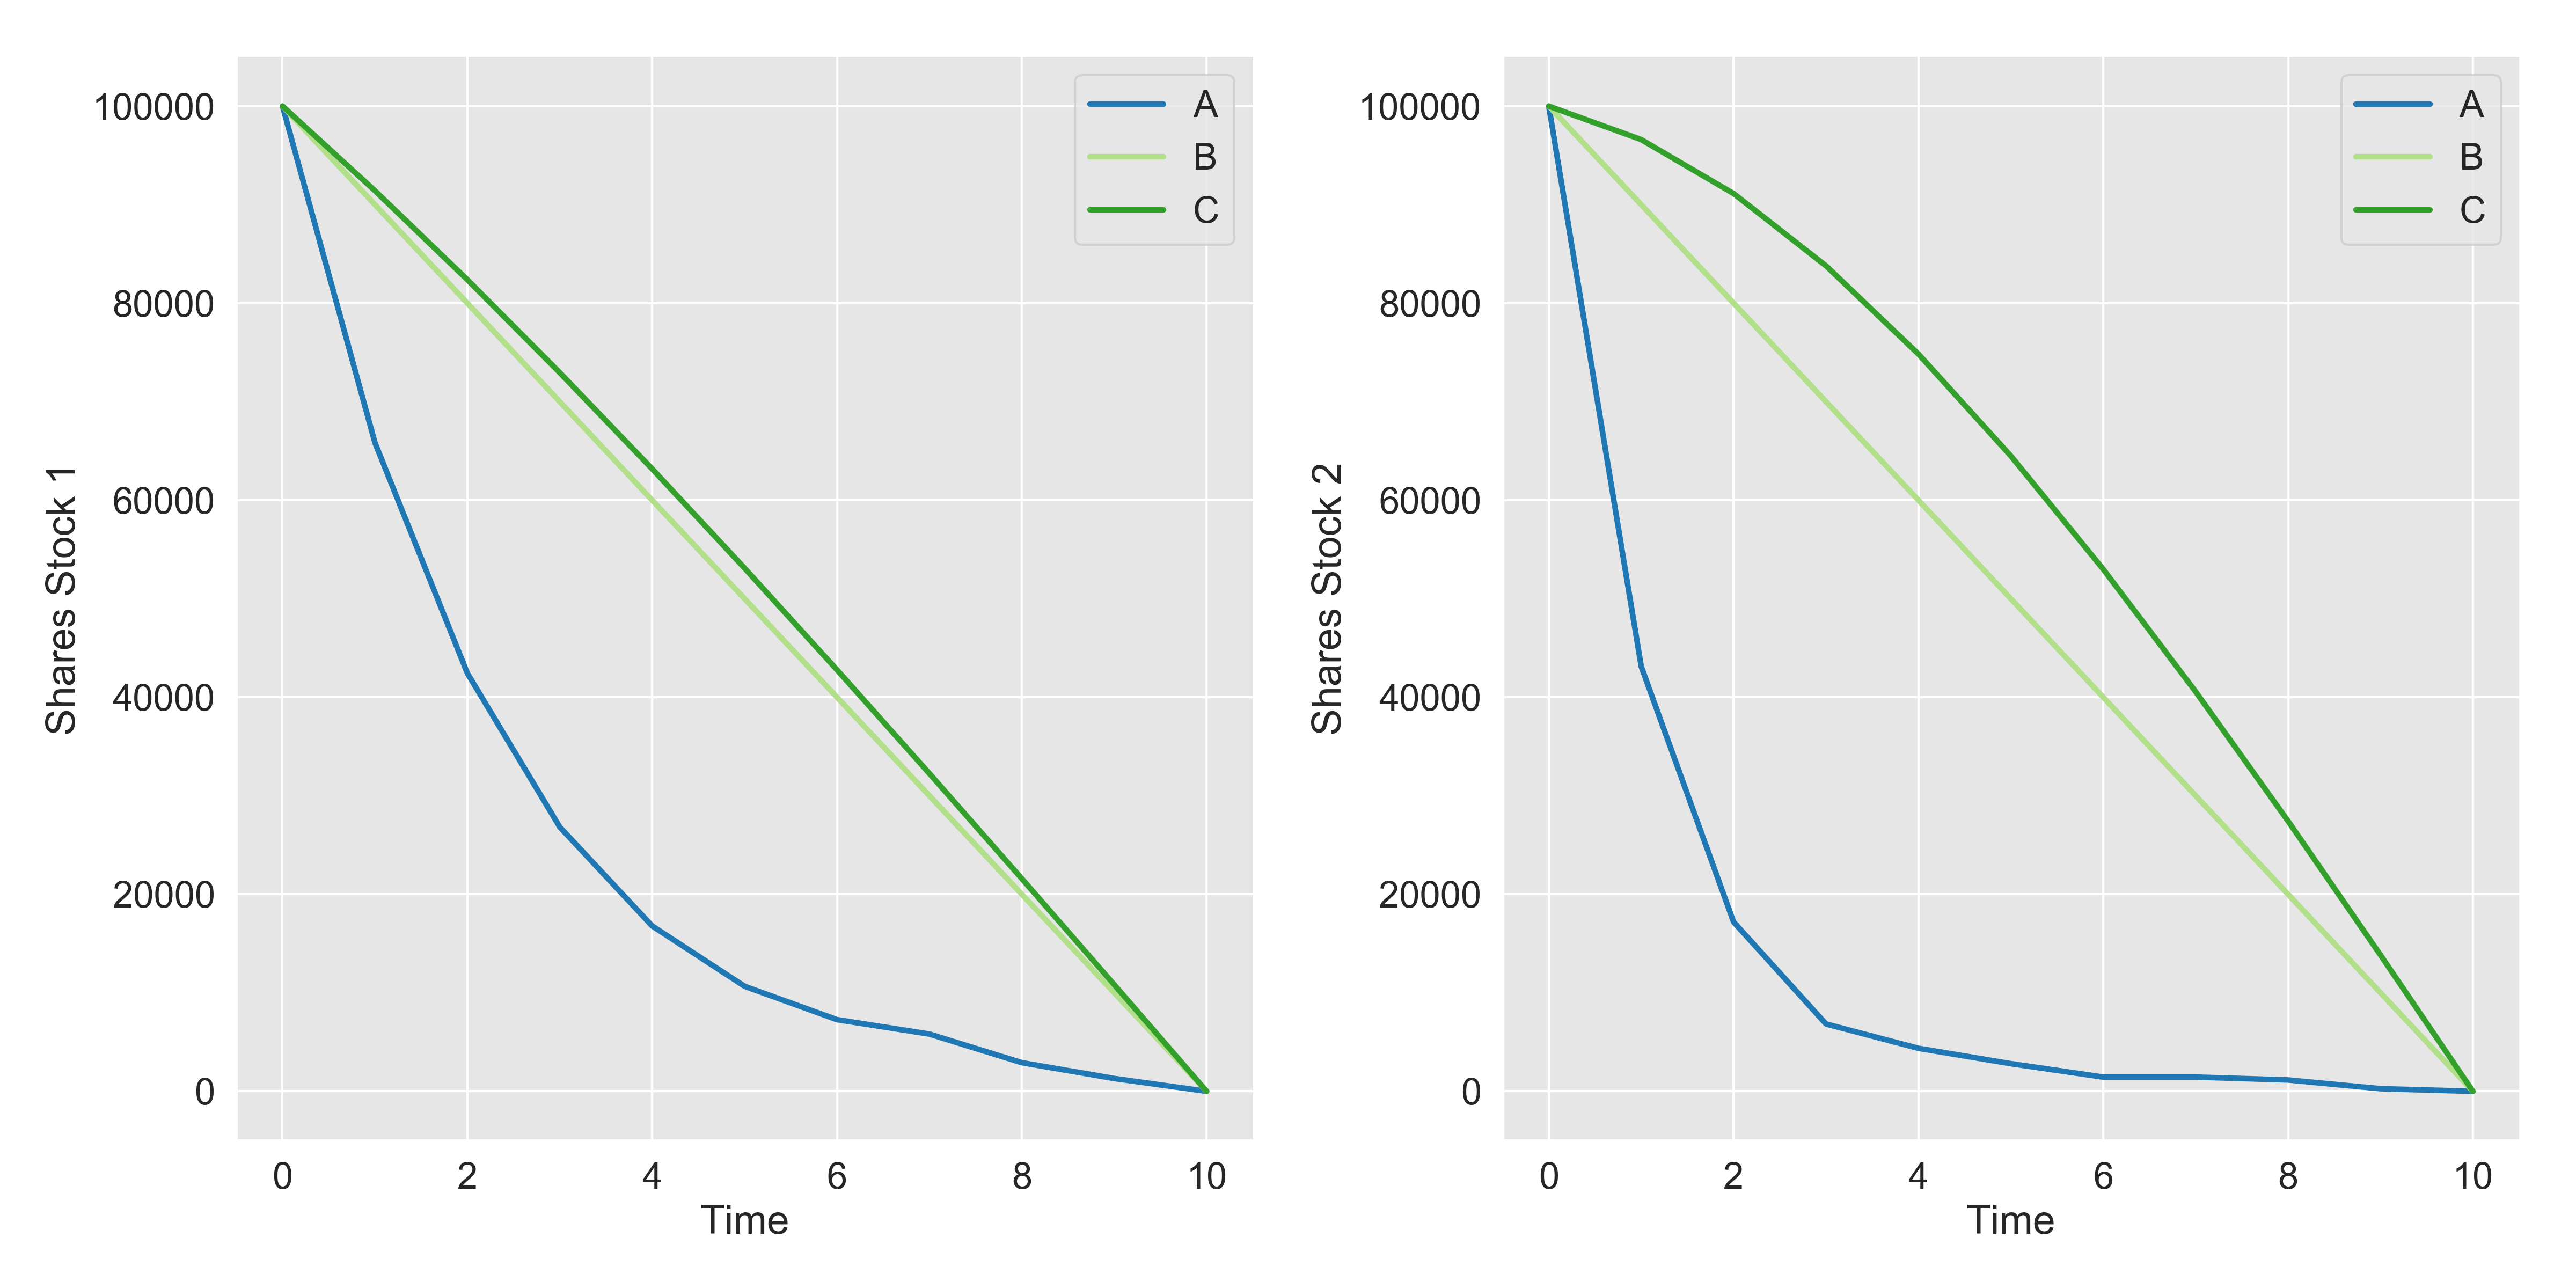
\includegraphics[width=\textwidth]{chapters/chapter_exec_models/figures/opt_traj1.png}
	\caption{Optimal Trajectories for two securities; ($A: \lambda= 2 \times 10^{-6}$; $B: \lambda=0$; $C= -5 \times 10^{-8}$; $B$ is the na\"ive strategy). \label{fig:7first}}
	\end{figure}
	\begin{figure}[!ht] 
	\centering
	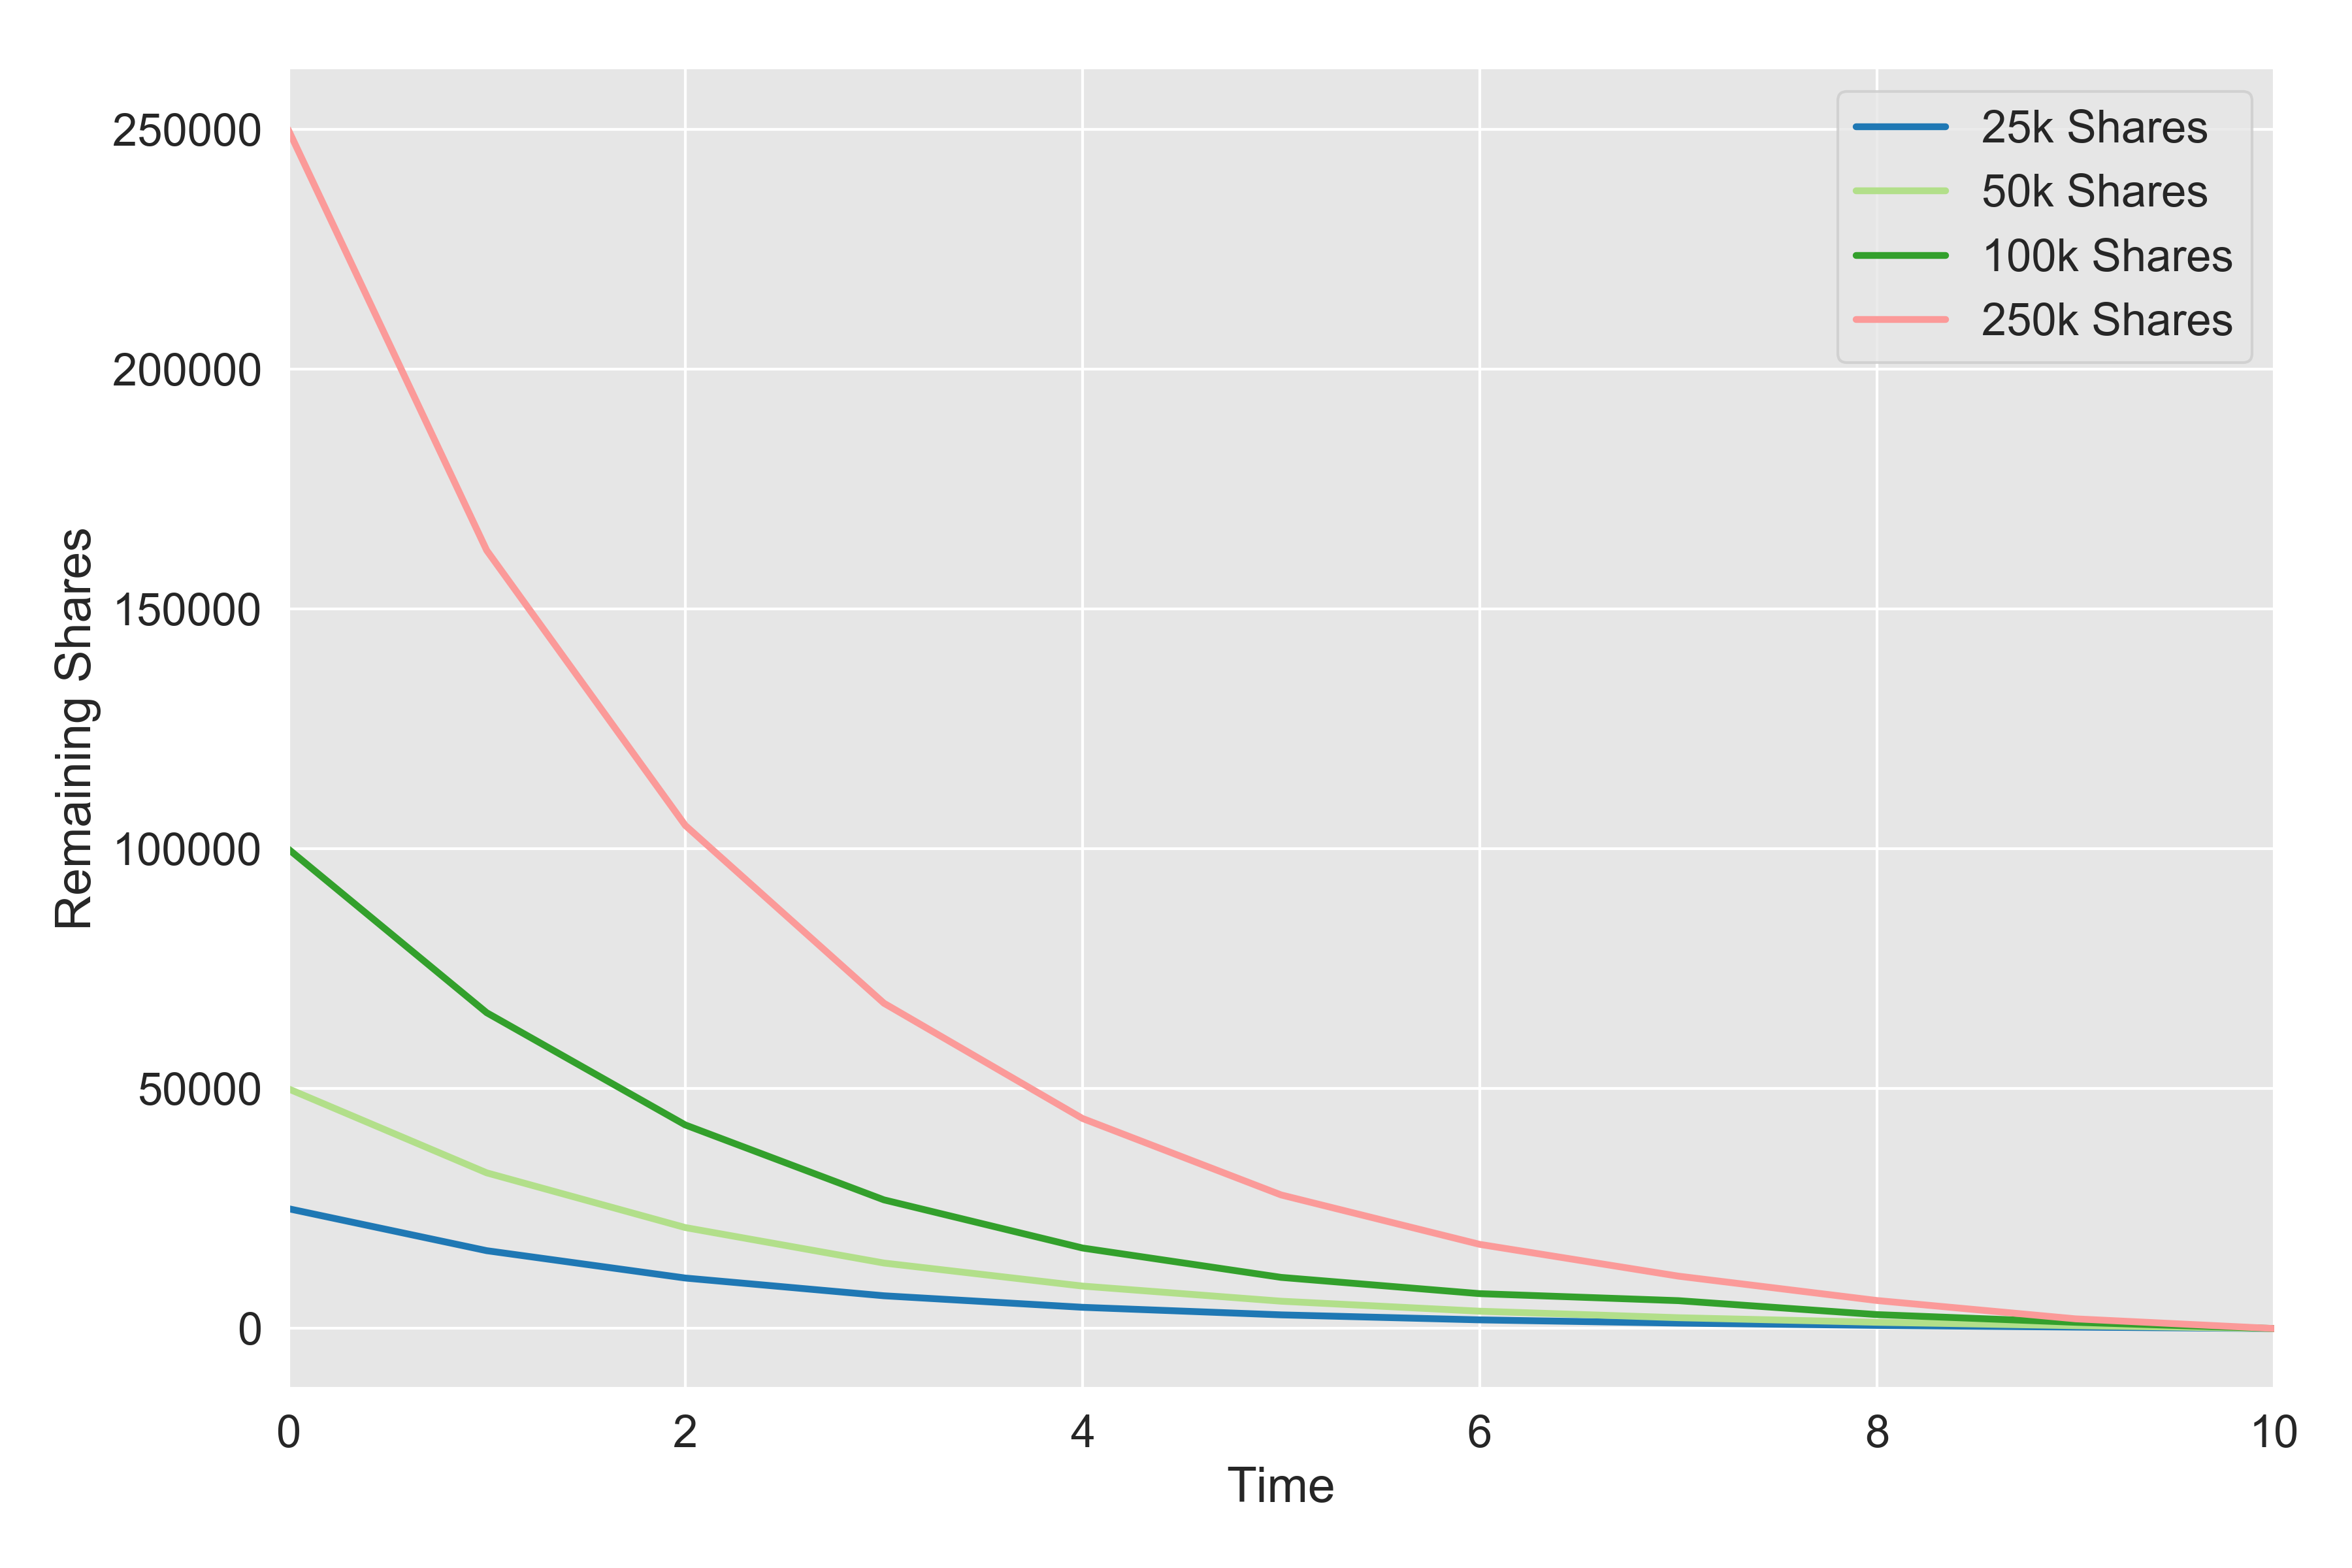
\includegraphics[width=\textwidth]{chapters/chapter_exec_models/figures/opt_traj2.png}
	\caption{Projected Execution Schedules \label{fig:7second}}
	\end{figure}
 

Some questions remain: what is the link between market impact and the dynamics of limit order book, is the impact function linear empirically, etc.. The effect of a short term drift in prices and the serial correlation in the errors which is observed in high frequency etc can be incorporated easily in the model \eqref{eqn:morepk}. Lorenz and Almgren (2011)~\cite{lovenz2011} provide a Bayesian approach to the optimization problem. While the methodology yields elegant solutions, empirical use of these results require a close monitoring of order book dynamics as the changes in demand and supply sides can be quite rapid. The general behavior of this adaptive strategy is aggressive; it depends on the prediction of short term price change; generally, if price goes up the tendency is to sell faster. 


The above mean-variance formulation of execution cost is combined with the traditional mean-variance portfolio optimization in Engle and Ferstenberg (2007)~\cite{engle2007} and Engle, Ferstenberg and Russell (2012)~\cite{engle2012}. We will discuss this in the context of portfolio rebalancing and the need for minimizing the transaction costs associated with all trades. While the above methods can be taken as first generation methods that are purely based on slippage, more recent work focus on adding other constraints such as incorporating the market VWAP and simultaneously determining the limit and market orders to achieve optimal results. \twomedskip


\noindent\textbf{Obizhaeva and Wang Model:} The models discussed in the previous sections assume price impact function that is not sensitive to liquidity dynamics. Obizhaeva and Wang (2013)~\cite{obizhaeva} develop a model that accounts for the dynamic properties of supply and demand as represented in the limit order book. An advantage of this approach is that the resulting strategies are likely to be robust to different order profiles. As advantage of this approach is that the resulting strategies are likely to be robust to different order profiles. The model captures `resilience'; that is, how the current trade affects the state of the future limit order book. The resulting strategy consists of a large trade initially aimed at moving the order book away from its steady state followed by a number of small trades that will utilize the inflow from new liquidity providers. The speed at which the book replenishes itself is an important part of execution cost. The level of resilience depends on the level of hidden liquidity in the market. The price impact model considered here takes into account the dynamics of the limit order book.


It is assumed that the parent order $X$ will be traded in the interval $(0,T)$, `$n$' times at $t_1, t_2, \ldots, t_n$. To model the execution of a large order in the limit order book, it is assumed that the price of execution ($p_t$) depends on the true value of the equity ($p_t^*$) and the state variables ($z_t$) such as past trades that may affect the book. Let $q(p_t^*,p_t;z_t)$ be the density of the limit orders in the other side of the book. The mid-quote ($\overline{p}_t$) is generally taken to reflect the true price, $p_t^*$. If the trade is on the buy side, the initial large transaction, $x_1$, can push the ask price to a higher level, $p_1^* + (s/2) + (x_1/q)$, where `$s$' is the spread and the average execution price is then equal to $p_1^* + (s/2) + x_1/(2q)$. After the initial execution the price converges to a new steady state, $p_t^*+s/2+\lambda x_1$. Assuming that the limit-order book converges to its steady-state exponentially and at time `$t$', 
	\begin{flalign} \label{eqn:qtdouble}
	&& q_t(p)&= q\cdot I(p>A_t) && \notag \\
	\text{and} && \phantom{x} & \phantom{x} && \\
	&& A_t&= \overline{p}_t + \dfrac{s}{2} + x_1 \cdot \kappa e^{-\rho t}, && \notag
	\end{flalign}
where $A_t$ is the asking price, $\kappa= 1/q - \lambda$ and `$\rho$' measures the resilience of the limit order book. If more the current ask price ($A_t$) deviates from steady state level, $\overline{p}_t + s/2$, the new ask limit orders will come into the book as the rate of $\rho \,q \,(A_t - \overline{p}_t - s/2)$. 


Given the above description of the limit order book dynamics, the optimal execution problem can be restated as follows:
	\begin{equation} \label{eqn:min}
	\min_{x_k} E_1\left( \sum_{k=1}^n [A_k + x_k(2q)] \,x_k \right),
	\end{equation}
such that $A_k= p_k^* + \lambda(X_1-X_n) + \dfrac{s}{2} + \sum_{i=1}^{k-1} x_i\ cdot \kappa e^{- \rho \tau(n-i)}$, where $p_k^*$, the true price is taken to follow a random walk.


The solution to this dynamic programming problem is given in Obizhaeva and Wang (2013)~\cite[p.14, Proposition 1]{obizhaeva} and is somewhat involved. Instead we state, the strategy when $n \to \infty$ which is of practical interest as many parent orders are divided into many, many child orders. The empirical market impact study that was presented in the last chapter attests to that. The solution to \eqref{eqn:min} as $n \to \infty$ are:
	\begin{equation} \label{eqn:orders}
	\begin{split}
	\text{First and final orders}: x_1&= \dfrac{X}{\rho_{T+2}} = x_n  \\
	\text{Spread of in-between trading}: x_t&= \dfrac{\rho x}{\rho_{T+2}}.
	\end{split}
	\end{equation}
The expected cost is determined as
	\begin{equation} \label{eqn:expected}
	\text{Expected cost}= \left( p_0^* + \dfrac{s}{2} \right) X_t + \lambda X_0 X_t + \alpha_t X_t^2 + \beta_t X_t D_t + \gamma_t D_t^2,
	\end{equation}
where $\alpha_t= \dfrac{\kappa}{\rho(T-t)+2} - \dfrac{\lambda}{2}$, $\beta_t= \dfrac{2}{\rho(T-t) + 2}$ and $\gamma_t= - \dfrac{\rho(T-t)}{2 \kappa[\rho(T-t) + 2]}$. The initial and final orders are discrete in nature and the orders in-between are continuous. They make use of incoming orders with favorable prices. 


Some comments are worth noting. Note the solution given in \eqref{eqn:orders} does not depend on the market depth, `$q$' and the price impact, `$\lambda$'. It is shown that the price impact is not a factor if the trade times are determined optimally and if they are not set a priori as in the other strategies. The reason for `$q$' not being a factor is due to the fact that the depth is taken to be constant at all times. This implies that there is enough liquidity in the market and the book gets replenished, albeit at a constant rate. The two factors that play important roles are the resiliency factor, `$\rho$' and the trading horizon, `$T$'. When $\rho=0$ the execution costs are strategy dependent and when $\rho \to \infty$, the order book rebuilds itself faster. When `$T$' increases, the size of the first and final order decreases; if there is more time to trade, the trades are spread out to manage the execution cost. The net cost of this strategy is
	\begin{equation}\label{eqn:netcost}
	\text{Net cost}=\dfrac{\lambda}{2} \cdot X^2 + \left(\dfrac{\kappa}{\rho_{T+2}}\right)^2 X^2
	\end{equation}
and it is shown to be smaller than the cost incurred if the strategy of constant rate trading is followed. 


Obizhaeva and Wang (2013)~\cite{obizhaeva} consider the extension of the optimization criterion in \eqref{eqn:min} to include the risk aversion as well, as in Almgren and Chriss (2000)~\cite{alm2000}. Interested readers should refer to Section~8 of their paper. For a practical implementation of these methods, it is necessary to consider the trading that happens in multiple exchanges and how the replenishment patterns can differ over different exchanges where `liquidity' and the fee structure have become major considerations for the order flow. \twomedskip


\noindent\textbf{Easley, De Prado and O'Hara Model:} In the models described so far in this section, it is assumed that the number of child orders `$n$' and the execution horizon, `$T$', are decided exogenously. Also the impact of a trade is modeled through the modified random walk model for the price with additional terms reflecting the permanent or temporary impact (Equations \ref{eqn:bigpk} and \ref{eqn:pdouble}). The process of how price impact arises due to friction in the liquidity access is an important part of market microstructure theory and this needs to be taken into account in determining the optimal execution. For example, a buyer in a seller's market can incur a lower cost of trading than a seller in a similar market. Obizhaeva and Wang model is based on the arrival dynamics to the order book. 


The approach taken by Easley, De Prado and O'Hara (2015)~\cite{prado2} is based on an asymmetric information model of the market maker's behavior. The key measure is the probability of information-based (PIN) trading that is estimated by the order book imbalance (see Easley, De Prado and O'Hara (2012)~\cite{prado3}). The premise is that selling a large order in a market already imbalanced toward sell, will reinforce adverse selection from the other side and thus widen the bid-ask spread resulting in higher market impact. The optimal execution horizon (OEH) model in Easley et al (2015) provide a framework for determining the trading horizon, `$T$', and does complement other earlier studies on execution strategies that minimize the price impact. 


The PIN that was developed in a series of papers (see Easley, Kiefer, O'Hara and Paperman (1996)~\cite{paper} and the references therein) views trading as a sequential game between liquidity providers and liquidity takers, repeated over the trading duration. If the information about the asset occurs with probability $\alpha$ and the chance that the information is good, is denoted by, $(1 - \delta)$ and further assume that the informed traders, who knew the terminal value of the asset under good news ($\overline{S}$) and under bad news ($\underline{S}$) arrive at the rate, $\mu$, and the noise traders arrive at the rate of `$\epsilon$'. The PIN is approximated as (assuming $\delta= 1/2$)
	\begin{equation} \label{eqn:pin}
	\text{PIN}= \dfrac{\alpha\mu}{\alpha\mu + 2\epsilon} \sim E[\text{OI}],
	\end{equation}
where order imbalance (OI), ($\text{OI}= \frac{V^B - V^S}{V}$), with $V$ denoting the volume. An aggressive buy order of size `$m$' can affect the order imbalance as
	\begin{equation} \label{eqn:oi}
	\text{OI}=\left( 2 \cdot \dfrac{V^B}{V} - 1 \right) \left(1 - \dfrac{m}{V} \right) + \dfrac{m}{V},
	\end{equation}
and note that $\left( 2 \cdot \frac{V^B}{V} - 1 \right)$ is the order imbalance, when $m= 0$, that is without the large trade. When `$m$' is small, the OI is likely to be perturbed too much and $m \to V$, that is the buy order will take all the available liquidity, then $\text{OI} \to1$. This also indirectly quantifies the amount of leakage or signaling that occurs with each trade.


An important factor that is associated with PIN is the range of liquidity that may exist in the market in the presence of both informed and noise traders:
	\begin{equation}\label{eqn:newsigma}
	\Sigma = \text{PIN} \cdot [\overline{S} - \underline{S}]
	\end{equation}
slicing a large order into small orders as suggested by earlier execution strategies does have timing risk and the asset price is assumed to follow a random-walk resulting in:
	\begin{equation}\label{eqn:randomwalk}
	\Delta S= \sigma \sqrt{\dfrac{V}{V_\sigma}} \, \xi,
	\end{equation}
where $\xi \sim N(0,1)$, $V_\sigma$ is the volume in the mid-price range. With `$\lambda$' as the probability of accepting a loss greater than $z_\lambda \cdot \sigma \cdot \sqrt{V/V_\sigma}$, the loss from trade size, `$m$', can be shown to be bounded by,
	\begin{equation}\label{eqn:bigbracp}
	P \left[ \dfrac{m \cdot \Delta s}{\hat{\sigma} \sqrt{\dfrac{V}{V_\sigma}}} > z_\lambda \right] = 1-\lambda
	\end{equation}
and thus `$\lambda$' can be interpreted as a `risk aversion' parameter. The OEH's goal is to determine the optimal trading volume, $V$, that can hide the purported trade, $m$, with minimum timing risk. The probabilistic loss function $\Pi$ that incorporates both liquidity and timing risk component is defined as:
	\begin{equation}\label{eqn:pi}
	\Pi = \left| \varphi(m) \cdot \text{OI} + (1-\varphi(m)) (2V^B-1)(\overline{S}-\underline{S})\right| - z_\lambda \sqrt{\dfrac{V}{V_\sigma}} \, \sigma.
	\end{equation}
Here $\varphi(m)$ is a monotonic function that maps into the range $(0,1)$. If `$V$' is greater, its impact is smaller in OI and larger in the trading range. The optimization results are given in Easley et al (2015)~\cite{prado2}.


The key quantities in determining the OEH are the order imbalance and the trade size/side. Figure~\ref{fig:3temp}, reproduced from Easley at al demonstrates how selling in a buyer's market allows for shorter horizons and in seller's market leads to longer horizons.  


        \begin{figure}[!ht] 
        \centering
        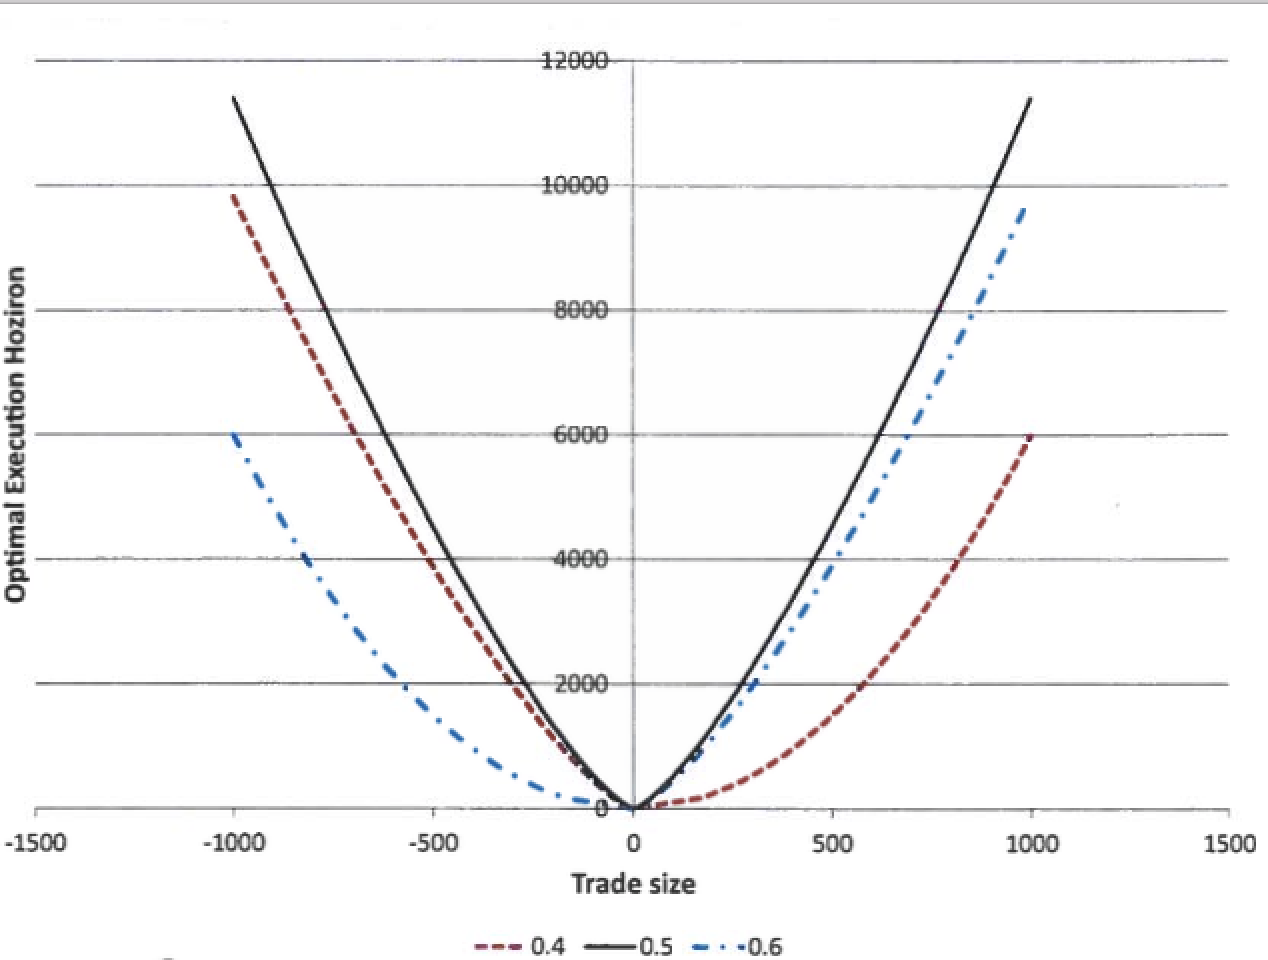
\includegraphics[width=\textwidth]{chapters/chapter_exec_models/figures/fig3temp.png}
         \caption{Optimal execution horizons for various order imbalances and trade sizes/sides. Combining alternative trade sizes and sides with our three scenarios ($v^B=0.4$, $v^B=\frac{1}{2}$, $v^B=0.6$) results in the optimal execution horizons displayed in the figure above, $\hat{\sigma}=1,000$, $V_\sigma=10,000$, $m=1,000$, $[\overline{S}-\underline{S}]=10,000$, $\lambda=0.05$ and $\varphi[|m|]$ linear. \label{fig:3temp}}
        \end{figure} \todo{nonscanned version?}



% Multiple Exchanges: Smart Order Routing Algorithm
\section{Multiple Exchanges: Smart Order Routing Algorithm \label{sec:mult_exch_sora}}

In the USA, there are over ten lit venues and close to forty dark venues and thus equity markets are highly fragmented. Each venue functions as an electronic limit order book of its own, where orders are prioritized first based on their prices and then at a given price level, according to their time of arrival. Exchanges publish information for each security in real-time and the information can change rapidly due to cancellations. The exchanges may differ with respect to best bid and offer price levels, the market depth at various prices etc. The exchanges also differ in their fee structures. Under the maker-taker pricing, exchanges offer rebates to liquidity providers and charge fees to takers of liquidity. These fees can range from $-\$0.001$ to $\$0.0030$. Because the typical bid-ask spread is $\$0.01$, the fees and rebates are a fairly significant fraction of the trading costs. Thus market participants must decide where child orders should be sent. It may be expensive to route to all the exchanges and by not routing to the right venue, it is possible to miss liquidity and hence incur greater market impact. At any point in time, the highest bid and the lowest offer among all exchanges comprise the National Best Bid and Offer (NBBO). Most traders use the smart order routing algorithms with goal to buy or sell the maximum number of shares in the shortest possible time with the least market impact possible. But a key issue is that many of the lit venues have hidden orders (12--45\%). How to estimate the size of the hidden orders and how to make routing decisions in the presence of hidden orders has been a focus of some recent research studies.


While exchanges compete along many fronts, for example, payment for order flow, transparency and execution speed, the key variables driving the efficiency are liquidity and price improvement. Thus the design of market structure is considered by market participants and regulators as the key determinant of flow of liquidity. The coexistence of multiple exchanges as mentioned in Parlour and Seppi (2003)~\cite{parlour2003} raises specific questions that are stated below:
        \begin{enumerate}[a)]
        \item Do liquidity and trading concentrate in a few exchanges?
        \item Do some market designs provide greater liquidity than others?
        \item Is the fragmentation of order flow desirable from a policy point of view?
        \item What is the constructive role for regulators to enhance liquidity?
        \end{enumerate}


Because exchanges operate under rules governing certain market designs, the performance and efficiency issues are related to the types of markets, such as pure limit order and a hybrid market (limit order book plus a specialist). In the hybrid market a specialist can provide supplementary liquidity after a market order has arrived. Parlour and Seppi (2003)~\cite{parlour2003} conclude only under some conditions such as enforcement of time priority, the efficiency is possible. Merely increasing the number of trading venues may result in degradation of market quality, if the enforcement of time priority is not followed, as it might discourage traders from posting the limit orders.


Foucault and Menkveld (2008)~\cite{foumen}consider the effect of fragmentation on two limit order markets. They examine the competition between Euronext and London Stock Exchange (LSE) in the Dutch market. The consolidated limit order book is found to be deeper after entry of the LSE. General conclusions from the above study and others such as Hendershott, Jones and Menkveld (2011)~\cite{hjm} and O'Hara and Ye (2011)~\cite{oye} are that fragmentation of order flows improves the liquidity supply and protecting orders against trade-throughs is important. Thus multiple exchanges are here to stay and smart order routing algorithms that can work well with the increased number of exchanges would be favorably sought by the market participants.


The smart order router (SOR), generally works as follows. A user can customize the use of the strategy by establishing a set of rules in splitting the parent order into child orders and the smart order routers are designed to ensure that the orders are routed to the venue with the best price and the orders are filled according to the trading strategies that may be pre-determined or may be adaptive. To be successful, SORs must be able to handle a variety of trading strategies and multiple venues. In addition they must deal with vast amount of incoming and historical market data. The publicly available information on the SORs used by major traders indicate that the order placement objective in general is to minimize client all-in shortfall with or without venue fees. The all-in shortfall consists of the shortfall on the filled shares and the cost of the clean-up trade for the unfilled shares. The latter is taken to be an important component of order placement optimization as it enables to quantify the effect of venue differences in fill rates, (see Street Smart, Issue 42, Jan 14, 2011). Other programs used in industry chose to optimize the expected time to execute the client's overall order. Expected queue speeds at various venues are predicted from recent trading data. Small orders tend to be placed in a single venue to minimize the queueing time whereas large orders will be placed in multiple venues to access maximum liquidity. In this model forecasting trading rates at different venues is crucial for successful implementation of the program. The rates are modeled as a function of lagged rates, thus capturing the momentum, and imbalances between supply and demand sides of the order book. Thus order placement in a fragmented market is not a trivial task.


A recent empirical study by Battalio, Corwin and Jennings (2016)~\cite{battcorjen} confirms that brokers use both limit and marketable orders to execute trades. Past studies provide evidence that market orders are sent to venues with lower trading costs and the trading fees and rebates generally affect consolidated market depth. Maglaras, Moallemi and Zheng (2012)~\cite{magmoazhe} show that limit orders are submitted to exchanges with high rebates and lower waiting time for execution while market orders are sent to venues that have lower fees and larger posted quote sizes. Cont and Kukanov (2017)~\cite{contk} develop a model that is somewhat more realistic to the current practice by decoupling the `order placement' decision from the scheduling decision and more importantly consider the option of placing limit orders on several exchanges, simultaneously. The model also accounts for the execution risk, the risk of not filling an order. Filling the unfilled portion may be costly and the allocation may shift toward market orders or toward overbooking, that is placing more orders than needed to refill.


To formalize the order placement problem, we assume a size of order $X$ is to be filled in the duration $(0,T)$. The decision is to split this order into a market order $M$ and `$K$' limit orders $L_1, \ldots, L_K$ with the same size to be placed in `$K$' exchanges with queue sizes $Q_1, \ldots, Q_K$ ; thus the order allocation is summarized by the elements of the vector $X=(M, L_1, \ldots, L_K)$ that need to be optimally determined. If order cancellations in the duration $(0,T)$ in exchange `$K$' is represented by $\xi_K$, then the number of shares transacted can be written as 
	\begin{equation} \label{eqn:axe}
	A(X,\xi)= M + \sum_{k=1}^K \left[ (\xi_k - Q_k)_+ - (\xi_k - Q_k - L_k)_+ \right],
	\end{equation}
where the terms in the parenthesis refers to the initial position and the final position of the queue outflows. The execution cost must account for fee ($f$) and rebate structures (discussed in Chapter~\ref{chap:ch_mi_models}) in each exchange and the cost of adverse selection ($r_k$) and can be stated as follows:
	\begin{equation}\label{eqn:cxe}
	C(X,\xi)= (h+f) M - \sum_{k=1}^K (h+r_k) \left[ (\xi_k - Q_k)_+ - (\xi_k - Q_k - L_k)_+ \right].
	\end{equation}
Here $h$ is one-half of bid-ask spread. 


The cost function in \eqref{eqn:cxe} can be modified to account for the cost of unfilled limit orders which may be filled through market orders at higher cost or it is possible that the prices have decreased resulting in additional adverse selection cost with penalty ($\lambda_u$) for falling behind and penalty ($\lambda_0$) for exceeding the target; Thus, the execution risk can be written as,
	\begin{equation}\label{eqn:er}
	\text{ER}= \lambda_u (S-A(X,\xi))_+ + \lambda_0 (A(X,\xi)-S).
	\end{equation}
To be more realistic, the market impact function can be considered as follows:
	\begin{equation}\label{eqn:mi}
	\text{MI}= \theta \left[ M + \sum_{k=1}^K L_k + (S-A(X,\xi))_+ \right].
	\end{equation}
The total cost function that includes both implicit and explicit costs can be states as:
	\begin{equation}\label{eqn:vxe}
	V(X,\xi)= C(X,\xi) + \text{ER} + \text{MI}.
	\end{equation}
The random variable in \eqref{eqn:vxe} is $\xi$, the cancellations that occur in various exchanges and the minimization function is $E[V(X,\xi)]$ with some assumed distribution for $F$ of $\xi$. Under some reasonable assumptions such as that the trader will not execute more than the target $X$ and market orders in the beginning of the duration $(0,T)$ are less expensive than at the end when unfilled orders are converted to market orders, an optimal solution is shown to exist (see Cont and Kukanov (2017)~\cite{contk} for details).


The analytical solution minimizing $V(X,\xi)$ is not easily tractable due to dimensionality issues. A numerical solution via gradient method is proposed. Random samples of $\xi$ are obtained and averaged to approximate $E(\xi)$. Let $q(X,\xi)= \Delta V(X,\xi)$ be the gradient of $V$. The following iterative algorithm is shown and converges:
	\begin{enumerate}[--]
	\item \textbf{Start with }$\mathbf{X_0}$\textbf{ and for }$\mathbf{n=1,2,\ldots,N}$\textbf{ do}
	\item $\mathbf{X_n=X_{n-1} - \gamma_N g(x_{n-1}, \xi^n)}$
	\item \textbf{End; }$\mathbf{X_N^* = \frac{1}{N} \sum_{n=1}^N X_n}$
	\end{enumerate}
The step size, \small
	\begin{equation} \label{eqn:7gammaN}
	 \gamma_N = \sqrt{k} S \left( N(h+f+\theta+\lambda_u +\lambda_0)^2 _ t + N \sum_{k=1}^K (h+r_k+\theta+\lambda_u+\lambda_0)^2 \right)^{-1/2} 
	\end{equation}
can be seen as a function of all the costs associated with the execution of the order.


To summarize, recall that the algorithm needs the following input:
	\begin{enumerate}[--]
	\item Trading Costs: 
		\begin{itemize}
		\item One half of bid-ask spread ($h$)
		\item Market order fee ($f$)
		\item Effective limit order risks ($r_k$)
		\item Market impact coefficient ($\theta$)
		\item Penalties for overfilling or underfilling ($\lambda_0,\lambda_u$)
		\end{itemize}
	\item Market Variables: Number of exchanges ($K$) and limit order queues ($Q_k$).
	\item Execution Variables: Time horizon ($T$) and target quantity ($S$).
	\end{enumerate}
While many of these quantities can be estimated using past transactions, the limit order queues ($Q_k$) and the cancellations ($\xi_k$) are to be obtained at the time of execution.



% Execution Algorithms for Multiple Assets
\section{Execution Algorithms for Multiple Assets}

The execution of trading entry-exit decisions can be made using the methods described in the earlier section for individual assets. Most investors hold multiple assets in their portfolios and evaluate their investments as a whole rather than in individual assets. In Section~\ref{sec:port_trad_strat}, we discussed the trading strategies with the focus on rebalancing the portfolios. The criteria used were in the traditional framework of mean-variance efficiency with some constraints on the transaction costs. When it comes to execution, the criteria as noticed from earlier sections is on execution costs and the market impact. We will briefly outline the issues related to execution of multiple-security portfolios.


%Only recently there are efforts made to better understand and model the cross-impact of trading an asset on trading of related assets. If a trader is liquidating simultaneously multiple assets as part of the rebalancing effort, we should expect some cross-impact. In the low frequency setting this is studied under `commonality' or `co-movement' as discussion in Chapter~\ref{ch:ch_mvts}. In the high frequency setting, the problem is harder to study due to short-term market frictions. A recent study by Schneider and Lillo (2019)~\cite{schnlillo19} extends the framework of Gatheral (2019)\todo{Missing reference} to multiple stocks where trading in one asset can impact the price of other assets. (More to follow.) 


The first form of multi asset execution we encountered was pairs strategies executing one side of a trade in proportion to the executions received on the other side. A natural extension of it is multi-leg algorithms where each side has multiple lines to be transacted over a certain horizon.


The implementation shortfall framework described previously relies on impact and risk dynamics of a single asset but can easily be extended to multiple assets. While the only real way to reduce risk in a single stock setup is to trade faster, in a portfolio scenario it is possible to control risk by exploiting the correlation structure across stocks. Portfolio algorithms aim to solve the execution dilemma (lowering impact cost at the expense of increasing timing risk exposure or vice versa) faced by traders of large baskets by offering two compelling sets of solutions:

        \begin{itemize}
        \item At comparable cost: reduce the risk by neutralizing market or factor exposures. 
        \item At comparable risk: reduce the cost by allowing slower trading than a list of individual IS strategies.
        \end{itemize}


Asset managers handle large trading lists when they periodically rebalance their holdings to tailor their exposure, or when they have inflows or outflows requiring to trade a sleeve of the portfolio. While this can present implementation challenges (such as managing cash neutrality between buys and sells across multiple markets), it also offers an opportunity for more efficient execution if the basket is traded in a coordinated fashion rather than as a list of independent single lines. Based on the trader view of what might be driving the short term risk of the portfolio during the execution window and their risk aversion, the trading schedules can be optimized along different risk-mitigating dimensions:

        \begin{itemize}
        \item Minimizing Country / Sector exposure
        \item Minimizing Factors exposure
        \item Minimizing Beta/Delta exposure
        \end{itemize}

(Most implementation leverage QP solvers and to create a flexible implementation for large portfolios that can be optimized in a reasonable time frame requires a lot of tricks and shortcuts)


From a pure trading implementation perspective, all the practical considerations mentioned in Chapter~\ref{s:pract_consid} apply to portfolio trading algorithms as well, in particular when handling the relative liquidity of the buy and sell sides. The complexity that is quite unique to portfolio trading is the handling of dark liquidity in the trade schedule optimization as it presents both an opportunity and a challenge. Similarly to a single line execution, finding a large block of liquidity in the dark allows to considerably reduce timing risk at a generally cheaper trading cost than would have been incurred in the lit market. That said, in a portfolio algorithm the trader relies on the correlation between names to balance the execution risk in order to slow down trading and minimize impact. So, receiving a large dark execution (or a series of simultaneous dark fills on the same side) at once can reintroduce significant risk by creating an imbalance, leaving the trader exposed to adverse market movements. The algorithm is then left to adjust its positions rapidly and might incur large execution costs to get back to a risk balanced state. This has two practical consequences for developers of portfolio algorithms. 


First, the names and quantities exposed to dark pools must be carefully selected to reflect the trade off between cost reduction at the single line level, risk reduction at the portfolio level, and potential cost incurred to return to a risk balanced portfolio. The scenarios encountered are as diverse as one can imagine and make the formulation of the problem harder once dark allocations are incorporated. To put things in perspective, we consider the two practical stylized examples as follow:


\begin{itemize}
\item A basket with a single position with a large percentage of ADV (i.e. large expected market impact) and small positions in liquid names (i.e. low expected market impact): in this scenario, the large percentage ADV order is the constraining factor in the execution speed of the whole portfolio, if that name can be traded as a block in the dark, it would allow the rest of the basket to trade faster (i.e. reducing exposure to timing risk) at little additional cost. --> posting dark as much as possible

\item A basket with a few names with a larger marginal contribution to risk (MCR)---but of not overly large notional sizes---and positions in liquid and illiquid names: in this scenario, executing the large MCR names would result in a better outcome only if the names paired off with them on the other side of the basket from a risk perspective are liquid enough to be executed rapidly at low cost. One possible way of assessing how much to post in the dark is to constrain the notional exposure with the available notional on the liquid names on the other side. That notional exposure can then be allocated among the large MCR names either na\"ively (equal split or in descending order of MCR) or applying a more sophisticated approach (for instance an allocation as a function of the MCR and the conditional probability of fill given the size allocated).
\end{itemize}


Second, when the portfolio incurs a sudden change in risk profile---whether due a dark fill or an abrupt market move in one direction---a reoptimization is necessary to return to a risk balanced position and to determine the new optimal trading schedules. This reoptimization can have different characteristics than the one that was performed at the beginning of the trade. Depending on the level of risk already exited up to that point in time, the trader as the ability to consider the temporary increase in risk as either something that needs to be reduced immediately in the next available trading bins, even if it generates larger trading costs, or something that can be reduced gradually in order to mitigate transaction costs. The optimal answer here also depends on the liquidity of the names still available to trade on the other side of the imbalance. \twomedskip


\noindent\textbf{Cross-Impact:} Only recently there are efforts made to better understand and model the cross-impact of trading an asset on trading of related assets. As mentioned earlier, if a trader is liquidating simultaneously multiple assets as part of the rebalancing effort, one should expect some cross-impact. In the low frequency setting when the focus is not necessarily on `execution' but on `trading', this is studied under `commodity' or `co-movement' as discussed in Chapter~\ref{ch:ch_mvts}, where the correlated changes are generally attributed to a general market factor that drives all the stocks. See Hasbrouck and Seppi (2001)~\cite{seppi2001}. In the high frequency setting, the problem is harder to investigate because of short-term market frictions. Almgren and Chriss (2000)~\cite{alm2000} discuss the extension of their execution algorithm to multiple assets, but this approach has not been followed up for a while. A recent study by Schneider and Lillo (2019)~\cite{schnlillo19} extends the single-stock framework of Gatheral (2010)~\cite{gatheral} to multiple stocks, but the formulation is in a continuous time framework. 



% Extending the Algorithms to Other Asset Classes
\section{Extending the Algorithms to Other Asset Classes}

While the electronification of trading first took place in the equity space, recent years have seen a significant growth of electronic trading and market making in the fixed income world, opening new opportunities to quantitative trading strategies. We give a brief overview of the characteristics of some of these products. \twomedskip


\noindent\textbf{(a)} \textbf{Options:} Historically, equity options markets have presented unique challenges to the successful deployment of sophisticated algorithmic trading strategies. First, options markets are significantly more fragmented than their equities counterparts, not just in space (i.e. across multiple exchanges) but also in terms of instruments. For one equity instrument representing a company (or for one index), there is a grid of available options over multiple maturities and multiple strike prices. Similarly to equities, options market data is disseminated in real time by the Options Price Reporting Authority (OPRA) which provides last sale reports and quotations from participant exchanges.\footnote{Options participant exchanges in OPRA: BOX Exchange, Cboe exchanges (BZX Options Exchange, C2 Options Exchange, EDGX Options Exchange, Options Exchange), Miami International Securities Exchange, MIAX PEARL, Nasdaq exchanges (BX, GEMX, ISE, MRX, PHLX, The Nasdaq Stock Market), NYSE exchanges (American, Arca).} OPRA is a national market system plan that governs the process by which options market data are collected from participant exchanges, consolidated, and disseminated. It also publishes other types of information with respect to the trading of options such as the number of options contracts traded, open interest and end of day summaries. 


One of the key challenges that remains in the options space is the amount of data generated on a daily basis, and the significant bursts that can happen when underlying equity markets move sharply and force a rapid adjustment of a myriad of correlated instruments. As an example, the OPRA message rates statistics\footnote{Source: \url{https://www.opradata.com/}} for the fourth quarter 2018 were: \twomedskip

\noindent Peak Messages Per Second (millions): $19.8$.

\noindent Peak Messages Per 100 Milliseconds (millions): $4.2$.

\noindent Peak Transactions Per Day (billions): $45.9$. \twomedskip


Automated options market making strategies were the first ones to be deployed, and we are now witnessing the emergence of execution strategies in the option space. For instance, targeting certain volatility levels (instead of price-based benchmarks). Given the natural relationship that exists with the underlying assets, options algorithmic trading strategies also require the implementation of automated delta and gamma hedging execution strategies.


It is also worth noting that most exchanges now support order types such as spreads making multi-leg strategies easier to implement. \twomedskip


\noindent\textbf{(b)} \textbf{Credit Derivatives:} When an entity, whether private or public, borrows money, the lender or debt holder bears some default risk until maturity. There is always a risk that the entity will not be able to repay the debt in full or per the agreed terms (coupons, maturity, \dots). Credit derivatives allow debt holders to hedge all or part of that risk, as well as speculators to express their views on the creditworthiness of various entities. 


A credit default swap (CDS) is a derivative contract allowing to buy or sell protection on a single reference entity. The protection buyer pays a fixed, running or upfront, a premium in return for the right to receive a payment should the reference entity suffer a credit event. Depending on the CDS contract, an eligible credit event might correspond to a payment default on the debt, a restructuring or a simple credit downgrade of the reference entity. In return for the premium, the writer of the CDS agrees to pay to the buyer (1---recovery rate) times the notional of the contract upon the realization of an eligible credit event. Here, the recovery rate represents the fraction of the face value of the debt that can be recovered following a credit event.


By entering a default swap, the buyer is essentially purchasing an insurance against the risk of default of a borrower. However, that insurance being paid by the CDS issuer bears counter-party risk (the ability of the issuer to pay the agreed amount in the event of a credit event affecting the borrower). Consequently, the valuation of a CDS depends, among other factors, on the default probability of the borrowing entity over the life of the contract, on the default probability of issuing counter-party, as well as the correlation between them.


The estimated CDS notional outstanding stands above $\$10$~trillions, after having peaked at about $\$62$~trillions at the end of 2007 (International Swaps and Derivatives Association (ISDA)), and north of 1~million trades are recorded per week. In the aftermath of the Global Financial Crisis of 2008, trading liquidity shifted from single name CDS toward CDS Indices, which are essentially baskets of single name CDS. Roughly half of the outstanding notionals originates from single reference entity contracts, while most of the other half emanates from credit indices (roughly $130,000$~trades per week in 2016).


Over-the-counter (OTC) derivatives markets are considered dealer markets, as they tend to be traded through a network of private dealers who stand ready to provide liquidity in various instruments while maintaining a relatively neutral net risk exposure. This, traditionally, is conducted one-on-one, off exchanges. However, the introduction of the Dodd-Frank Act of 2010 brought significant transformation to the U.S. swap markets by mandating central clearing for standardized over-the-counter derivatives such as swaps, as well as forcing their execution on a swap execution facility (SEF).\footnote{In Europe, the MiFID II directive adopted by the EU in 2014, with applicability on January 3rd, 2018, also introduces obligations for sufficiently liquid standardized derivatives contracts to be traded only on regulated platforms such as OTFs: Organized Trading Platform.}


The term `swap execution facility' defines a registered ``trading platform in which multiple participants have the ability to execute or trade swaps by accepting bids and offers made by multiple participants'' (Dodd-Frank Act, Section 733). Among the stated goals of mandating swaps execution on SEFs are: promoting pre-trade transparency in the swaps market as well as facilitating the real-time publication of trading information such as price and volume to enhance price discovery. As such, the Dodd-Frank Act addressed for swap markets, the three main challenges that had historically prevented a significant electronification of trading in fixed income markets: lack of standardized instruments, lack of centralized trading platforms and lack of available transaction data.


SEFs usually offer multiple trading protocols giving investors the flexibility to choose the most appropriate trading style for their needs. Existing trading protocols center around either an Order Book-like approach where all market participants have the ability to execute available bids or offers from multiple participants as well as leave their own limit orders; or a Request-For-Quote (RFQ)-like approach where participants request a single or two-sided market from multiple dealers during a real-time auction.


A variety of credit Indices are fairly liquid and trading on SEFs, in particular U.S. indices (CDX(c)) and European indices (iTraxx(c)). The CDX indices are further broken out by the type of debt covered such as Investment Grade (IG) and High Yield (HY) for the most liquid ones. Due to their liquidity, both CDX IG and CDX HY are examples of credit indices that lend themselves well to electronic market making activities.


However, the CDS Index market presents a certain number of idiosyncrasies compared to equity markets when it comes to market making. While there is an order book available to all participants, most of the volume still gets transacted via RFQ mechanism for which market makers are not always allowed to see the quotes. Consequently, market makers only have partial information regarding the true position of the market when time comes to decide where to place their own orders. Using a mixture of historical trades and partial real-time information, market makers can reconstruct a theoretical mid price of the market. They can set then the bid and ask quotes at an appropriate distance from that mid price, accounting for the trade-off between their desire to obtain a fill and the risk associated with maintaining their inventory. \twomedskip


\noindent\textbf{(c)} \textbf{Corporate Bonds:} The corporate bond market is also an OTC market where market participants only have access to limited information prior to placing a trade. The major market participants are pension funds and insurance companies which tend to have longer investment horizons, hedge funds which tend to have more tactical trading allocations, and corporate treasury departments whose objectives and horizons can span a wide spectrum.


Compared to other assets, it is also interesting to note that most of the secondary market transactions happen in the first few months following issuance, and after that a significant portion of the amount of bonds issued is held to maturity. Similarly to other fixed income products, the key challenges for secondary trading of bonds and the electronification of its secondary markets have historically been lack of centralized market place, lack of harmonized instrument characteristics and lack of transaction data.


The corporate bonds secondary market remains dominated by one-to-one privately negotiated trades, but electronic platforms allow transacting via similar execution protocols as what traders can use for CDSs: limit order book type of executions as well as request-for-quotes (RFQ) on platforms such as Tradeweb, Bloomberg, MarketAccess among others.


In the U.S., for instance, under FINRA Rule~6730, Broker-dealer FINRA member firms have the obligation to report transactions in TRACE-eligible securities to the TRACE\footnote{Trade Reporting And Compliance Engine.} database as early as practically possible, but no later than within 15~minutes of the Time of Execution. FINRA Rule~6710 defines TRACE-eligible securities as USD denominated debt securities (whether issued by a U.S or foreign private issuer), and USD denominated debt issued or guaranteed by an Agency or Government-Sponsored Enterprise. Foreign sovereign, U.S. Treasuries and money market instruments are specifically excluded from the eligible list. The TRACE database then disseminates price, size,\footnote{The actual size disseminated back to the market is capped to prevent excessive information leakage: for investment-grade corporate bonds and agency debt securities, for any trade greater than \$5~million, the par value is displayed as \$5~MM$+$; for non-investment grade corporate bond, the displayed quantity is capped to \$1~million par value.} time stamp and direction of the trade to the public. While the rules require reporting in no more than 15~minutes, most reporting and public dissemination now happens within seconds or minutes of execution (with the exception of overnight trades being batch-reported the next morning), giving participants some transparency about the current market levels.


The combination of existing venues allowing for click-to-trade or RFQ protocols and trade events information facilitated the expansion of electronic trading for corporate bonds as well. A fifth to a quarter of the investment grade market is now transacted electronically, while on the high yield side, roughly 10\% of the market is traded through RFQs.


Similarly to credit indices, the first challenge for dealers in corporate bond electronic market making is to infer the value of the current ``fair mid'' for the market following each transaction. Given the relatively infrequent updates observations even for bonds that are considered liquid, quantitative techniques employed tend to vary from the ones used in markets with higher frequency data available such as equities. Practitioners rely much more, for instance, on probabilistic state-space models to estimate unobservable state variable.


This type of approach obviously becomes increasingly more challenging as one moves down the liquidity spectrum. It is not uncommon for illiquid bonds to not trade for months, in which case assessing a fair mid price cannot solely rely on prior transactions. Among possible solutions, modelers can use bonds of other maturities from the same issuers, or bonds from correlated issuers or comparable investment grades. Additionally, more liquid credit derivatives are also a potential sources of information that can be leveraged for better valuations. 



%\noindent\emph{Stochastic Adaptive Control Approach to Optimal Execution}
%\noindent\emph{Reinforcement Learning}
% The Future of Execution Strategies
\section{The Future of Execution Strategies}

\begin{comment}
\todo{Do we want to talk about the next generation}
In order to develop an execution strategy achieving the objective(s) prescribed by the given benchmark(s), the execution problem can be modeled as a multi-step Markov decision process. However, the dimensionality of the problem explodes rapidly given the quasi infinite size of the state space (to represent the market), the large number of steps (even simplifying to 1s resolution, it results in over 20,000 steps for U.S. equities - compared, for instance, to an average of only 40 moves per chess game\footnote{Chessgames database: www.chessgames.com/chessstats.html}) and also the large size of the action space. To address this complexity, most execution algorithms decompose the problem into different timeframe decisions such as scheduling, placement and routing. 
\end{comment}
